%%% Kompilieren mit:
%%%
%%%   0) Auswählen unten: \querverweisetrue oder \querverweisefalse
%%%   2) pdflatexuli -n -s -b emradscope_docu.tex 3

%%% machemireinpdf so lassen! Läuft derzeit nur mit pdflatex, weil
%%% sich manche eingebundenen PDF-Graphiken nicht so einfach 
%%% in "kleine" EPS wandeln lassen!
\newif\ifmachemireinpdf
%\machemireinpdffalse  %%% Fuer lauf mit latexuli -n -b artif_docu.tex 3
\machemireinpdftrue    %%% Fuer lauf mit pdflatexuli  -n -b artif_docu.tex 3

\newif\ifquerverweise
%\querverweisefalse     %%% ohne hyperref-Querverweise fuer Druck (bei PDF)
\querverweisetrue      %%% mit hyperref-Querverweisen zum Lesen am Bildschirm (bei PDF)


% Wegen veraltetem KOMA-Skript notwendig, wenn hyperref, bookmark oder
% aehnliches verwendet wird. Noetig, wenn latex mit der Fehlermeldung 
% "! Package ifvtex Error: Name clash, \ifvtex is already defined." abbricht.
%\RequirePackage{ifvtex}

\documentclass[10pt,a4paper,twoside,headinclude,footinclude,parskip=half]{scrartcl}

\usepackage{ifpdf}

\usepackage[a4paper,twoside,portrait,hmargin={1.2in,1.0in},vmargin={1.0in,1.0in},footskip=2.5em]{geometry}

%\usepackage{scrpage2}
\usepackage{scrlayer-scrpage}

\usepackage[english]{babel}
\usepackage[OT1]{fontenc}
\usepackage[utf8]{inputenc}


\newif\ifquerverw
\ifmachemireinpdf
  \ifpdf
    \ifquerverweise
      \querverwtrue
    \else
      \querverwfalse
    \fi
    \pdfoutput=1 % we are running pdflatex 
    \pdfcompresslevel=5     % compression level for text and image;
    \ifquerverw
    \usepackage[pdftex,colorlinks=false,pdfpagelayout=SinglePage,pdffitwindow=true]{hyperref}
    \fi
  \fi
\else
  \querverwfalse
\fi

\usepackage{xspace}
\usepackage{calc,ifthen}
\usepackage{array,longtable,multicol,hhline,afterpage}
\usepackage[fleqn]{amsmath}
\usepackage{amssymb}
\usepackage{graphicx,color}

\usepackage[savemem]{listings}
\usepackage{fancyvrb}

\usepackage{enumitem}

\usepackage[lined,longend]{algorithm2e}

\usepackage{natbib}

%%% treat _ in textmode correctly (you don't have to \_ any more ...)
%%% However, in order of _ still working in, e.g., included filenames,
%%% you need to provide the option "strings", see the documentation of
%%% the underscore-package! For citation tags there is the same problem, but
%%% they are not automatically protected. For this you need also
%%% to do a \newcommand{\UnderscoreCommands}{ \do\citeNP \do\shortciteN ...}
%%% before loading "underscore".
%%% The same holds true for \bibliographystyle, which triggers the use of \bibstyle.
\newcommand{\UnderscoreCommands}{\do\citet \do\citeauthor \do\citeyear \do\bibliographystyle \do\bibstyle}
\usepackage[strings]{underscore}


% Print the word "draft" or a watermark picture at the background of each page:

%%% possiblilities: packages draftcopy, draftwatermark, everypage, wallpaper, ...

% \ifquerverw
% \usepackage{draftwatermark}
% \SetWatermarkAngle{60}
% %% Lightness of the watermark text (1=white, 0=black)
% \SetWatermarkLightness{0.8}
% %% Font size of the watermark text
% \SetWatermarkFontSize{5cm}
% %% Scaling of the watermark text
% \SetWatermarkScale{10.0}
% %%Watermark text 
% \SetWatermarkText{Draft}
% \fi

%\usepackage{wallpaper}
%% %\CenterWallPaper{0.9}{watermark.png}


%Zeilenabstand einstellen:
\linespread{0.95}

\pagestyle{scrheadings}
%%% \ifoot[<das passiert bei scrplain>]{<das passiert bei scrheadings>}
\ifquerverw%
  \newcommand{\myaktuellesection}{sec:intro}%
  \newcommand{\myaktuellesubsection}{sec:intro}%
  \newcommand{\labelsec}[1]{\label{#1}\renewcommand{\myaktuellesection}{#1}}%
  \newcommand{\labelsubsec}[1]{\label{#1}\renewcommand{\myaktuellesubsection}{#1}}%
\else
  \newcommand{\labelsec}[1]{\label{#1}}%
  \newcommand{\labelsubsec}[1]{\label{#1}}%
\fi
\automark[section]{subsection}%
\ihead[]{}%
\ohead[]{\headmark}%
\chead[]{}%
\ifquerverw%
  \ifoot[]{\autoref{\myaktuellesection}\xspace\quad\autoref{\myaktuellesubsection}\xspace\quad%
    \hyperref[sec:inhalt]{TOC}\xspace\quad \hyperref[sec:nml]{Namelists}\xspace}%
\else%
  \ifoot[]{}%
\fi%
\cfoot[]{}%
\ofoot[\pagemark]{\pagemark}%
\setheadsepline{1pt}%

\setlength{\emergencystretch}{20pt}
\tolerance=2000
\frenchspacing

% % Disable single lines at the start of a paragraph (Schusterjungen)
\clubpenalty = 10000

% Disable single lines at the end of a paragraph (Hurenkinder)
\widowpenalty = 10000 \displaywidowpenalty = 10000


% Define own macros here:
\newcommand{\pabl}[3][]{\ensuremath{\dfrac{\partial^{#1} #2}{\partial #3^{#1}}}\xspace}
\newcommand{\pablS}[4][]{\ensuremath{\left.\dfrac{\partial^{#1} #2}{\partial #3^{#1}}\right|_{#4}}\xspace}
\newcommand{\mpunkt}{\quad\text{.}}%
\newcommand{\mkomma}{\quad\text{,}}%
\newcommand{\gleichundhiergehtein}[1]{\underset{\underset{\makebox[0pt]{\ensuremath{#1}}}{\Big\uparrow}}{=}}% nur math-mode!
\newcommand{\grad}{\ensuremath{^{\circ}}\xspace}
\newcommand{\gradC}{\ensuremath{^{\circ}\,C}\xspace}

\newcommand{\citeP}[1]{\citet{#1}} 
\newcommand{\citeNPK}[1]{\citeauthor{#1}, \citeyear{#1}}

\ifquerverw
% \renewcommand{\sectionname}{Section}
 \renewcommand{\sectionautorefname}{Section}
% \renewcommand{\subsectionname}{Subsection}
 \renewcommand{\subsectionautorefname}{Subsection}
% \renewcommand{\pagename}{Seite}
 \renewcommand{\figurename}{Figure}
 \renewcommand{\figureautorefname}{Figure}
 \renewcommand{\tablename}{Table}
 \renewcommand{\tableautorefname}{Table}
\fi

\ifquerverw
  \newcommand{\refgl}[1]{\hyperref[#1]{(\ref*{#1})}\xspace}%
  \newcommand{\glg}[1]{\hyperref[#1]{equation~(\ref*{#1})}\xspace}%
  \newcommand{\GLG}[1]{\hyperref[#1]{Equation~(\ref*{#1})}\xspace}%
  \newcommand{\seite}[1]{\hyperref[#1]{\pagename~\pageref*{#1}}\xspace}
  \newcommand{\abb}[1]{\autoref{#1}\xspace}%
  \newcommand{\abschnitt}[1]{\autoref{#1}\xspace}
  \newcommand{\tabelle}[1]{\autoref{#1}\xspace}
  \newcommand{\querverweis}[2]{\hyperref[#1]{#2}\xspace}

\else
  \newcommand{\refgl}[1]{(\ref{#1})\xspace}%
  \newcommand{\glg}[1]{equation~(\ref{#1})\xspace}%
  \newcommand{\GLG}[1]{Equation~(\ref{#1})\xspace}%
  \newcommand{\seite}[1]{\pagename~\pageref{#1}\xspace}
  \newcommand{\abb}[1]{figure~\ref{#1}\xspace}%
  \newcommand{\ABB}[1]{Figure~\ref{#1}\xspace}%
  \newcommand{\abschnitt}[1]{section~\ref{#1}\xspace}
  \newcommand{\ABSCHNITT}[1]{Section~\ref{#1}\xspace}
  \newcommand{\tabelle}[1]{table~\ref{#1}\xspace}
  \newcommand{\TABELLE}[1]{Table~\ref{#1}\xspace}
  \newcommand{\querverweis}[2]{{#2}\xspace}
\fi

\newlength{\tmplena}%
\newlength{\tmplenb}%

\newenvironment{aufzaehlung}%
{\begin{list}{$\bullet$}{%
      \setlength{\labelwidth}{8mm}%
      \setlength{\leftmargin}{\labelwidth*\real{0.5}}%
      \setlength{\tmplena}{\itemsep}%
      \setlength{\itemsep}{0mm}%
}}{\setlength{\itemsep}{\tmplena}\end{list}}%


\newcommand{\srcform}[1]{\mbox{\texttt{#1}}\xspace}%
\newcommand{\paramform}[1]{\mbox{\texttt{#1}}\xspace}%


%%%%%%%%%%%%%%%%%%%%%%%%%%%%%%%%%%%%%%%%%%%%%%%%%%%%%%
%%% SOME NECESSARY MACROS FOR THE INCLUDED TABLES:
%%%%%%%%%%%%%%%%%%%%%%%%%%%%%%%%%%%%%%%%%%%%%%%%%%%%%%

\newlength{\tmplenaq}
\newlength{\tmplenbq}

%%%%%%%%%%%%%%%%%%%%%%%%%%%%%%%%%%%%%%%%%%%%%%%%%%%%%%%%%%%%%%%%%%%%%%%%%
%%% New lengths variables for the column widths (\linewidth) for table cells:
%%%%%%%%%%%%%%%%%%%%%%%%%%%%%%%%%%%%%%%%%%%%%%%%%%%%%%%%%%%%%%%%%%%%%%%%%

\newlength{\lenspeins}%   Column 1, to be actually set before the table
\newlength{\lenspzwei}%   Column 2
\newlength{\lenspdrei}%   Column 3
\newlength{\lenspvier}%   Column 4
\newlength{\lenspfunf}%   Column 5

%%%%%%%%%%%%%%%%%%%%%%%%%%%%%%%%%%%%%%%%%%%%%%%%%%%%%%%%%%%%%%%%%%%%%%%%%
%%% Compress texts to the column width (\linewidth) for table cells:
%%%%%%%%%%%%%%%%%%%%%%%%%%%%%%%%%%%%%%%%%%%%%%%%%%%%%%%%%%%%%%%%%%%%%%%%%

\newcommand{\quetsche}[1]{%
\setlength{\tmplenaq}{\widthof{#1}}%
\ifthenelse{\lengthtest{\tmplenaq > \linewidth}}{%
\resizebox{\linewidth}{\height}{{#1}}}%
{{#1}}%
}

%%%%%%%%%%%%%%%%%%%%%%%%%%%%%%%%%%%%%%%%%%%%%%%%%%%%%%%%%%%%%%%%%%%%%%%%%
%%% Similar for multicolumns(2) cells:
%%%%%%%%%%%%%%%%%%%%%%%%%%%%%%%%%%%%%%%%%%%%%%%%%%%%%%%%%%%%%%%%%%%%%%%%%

\newcommand{\quetschee}[1]{%
\setlength{\tmplenaq}{\widthof{#1}}%
\setlength{\tmplenbq}{\lenspeins + \lenspzwei + 2\tabcolsep}%
\ifthenelse{\lengthtest{\tmplenaq > \tmplenbq}}{%
\resizebox{\tmplenbq}{\height}{{#1}}}%
{{#1}}%
}

%%%%%%%%%%%%%%%%%%%%%%%%%%%%%%%%%%%%%%%%%%%%%%%%%%%%%%%%%%%%%%%%%%%%%%%%%
%%% Enclose cells with a certain format:
%%%%%%%%%%%%%%%%%%%%%%%%%%%%%%%%%%%%%%%%%%%%%%%%%%%%%%%%%%%%%%%%%%%%%%%%%

\newcommand{\spvierformat}[1]{%
\parbox[t]{\linewidth}{#1}%
}

%%%%%%%%%%%%%%%%%%%%%%%%%%%%%%%%%%%%%%%%%%%%%%%%%%%%%%
%%% Customize the itemize-environm. for the tables:
%%%%%%%%%%%%%%%%%%%%%%%%%%%%%%%%%%%%%%%%%%%%%%%%%%%%%%

\newenvironment{tabitemize}
{\begin{list}{$\bullet$}{
    \setlength{\labelwidth}{\widthof{2 =}}
    \setlength{\labelsep}{1ex}
    \setlength{\leftmargin}{\labelwidth+\labelsep}
    \setlength{\itemsep}{0.2em plus 0.1em minus 0.2em}
    \setlength{\parsep}{0mm}
    \setlength{\topsep}{0.2em plus 0.1em minus 0.2em}
    \setlength{\partopsep}{0mm}
  }}{
\end{list}}%

\newenvironment{tabitemizeindent}[1]
{\begin{list}{$\bullet$}{
    \setlength{\labelwidth}{#1}
    \setlength{\labelsep}{1ex}
    \setlength{\leftmargin}{\labelwidth+\labelsep}
    \setlength{\itemsep}{0.2em plus 0.1em minus 0.2em}
    \setlength{\parsep}{0mm}
    \setlength{\topsep}{0.2em plus 0.1em minus 0.2em}
    \setlength{\partopsep}{0mm}
  }}{
\end{list}}%

\definecolor{blau}{rgb}{0.0,0.0,1.0}


\title{EMVORADO --- Efficient Modular VOlume scan RADar Operator}
\subtitle{\Huge --- A User's Guide ---}
\author{Ulrich Blahak$^{1,2}$, Alberto de Lozar$^{2}$, Jana Mendrok$^{2}$}
\date{\today\\[0.8em]\parbox[t]{\linewidth}{\centering (Contributors to EMVORADO development see imprint on next page)}}

\begin{document}

%%%% Nice looking title page:

\maketitle

\setlength{\unitlength}{1cm}
\newcommand{\scalfakt}{2.2}  % for polarimetric variables fontwork
\begin{picture}(0,15.2)(0,0)
\put(1.0,5.0){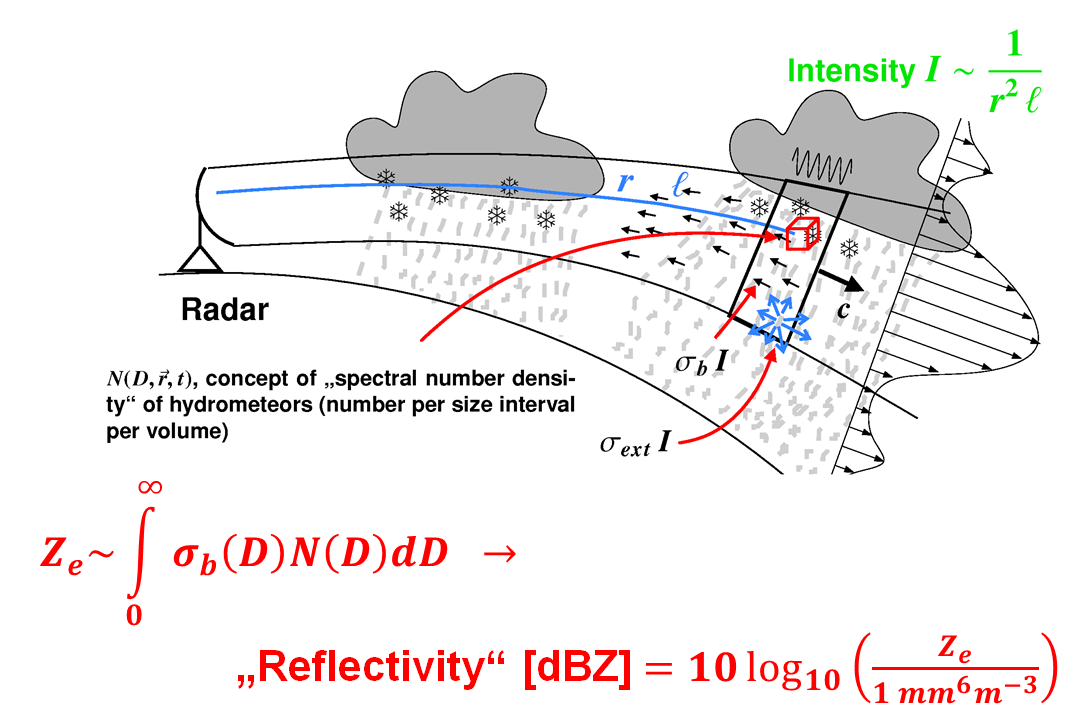
\includegraphics[width=\linewidth*\real{0.95}]{radar_principle_ray.png}}
\put(-2.0,12.0){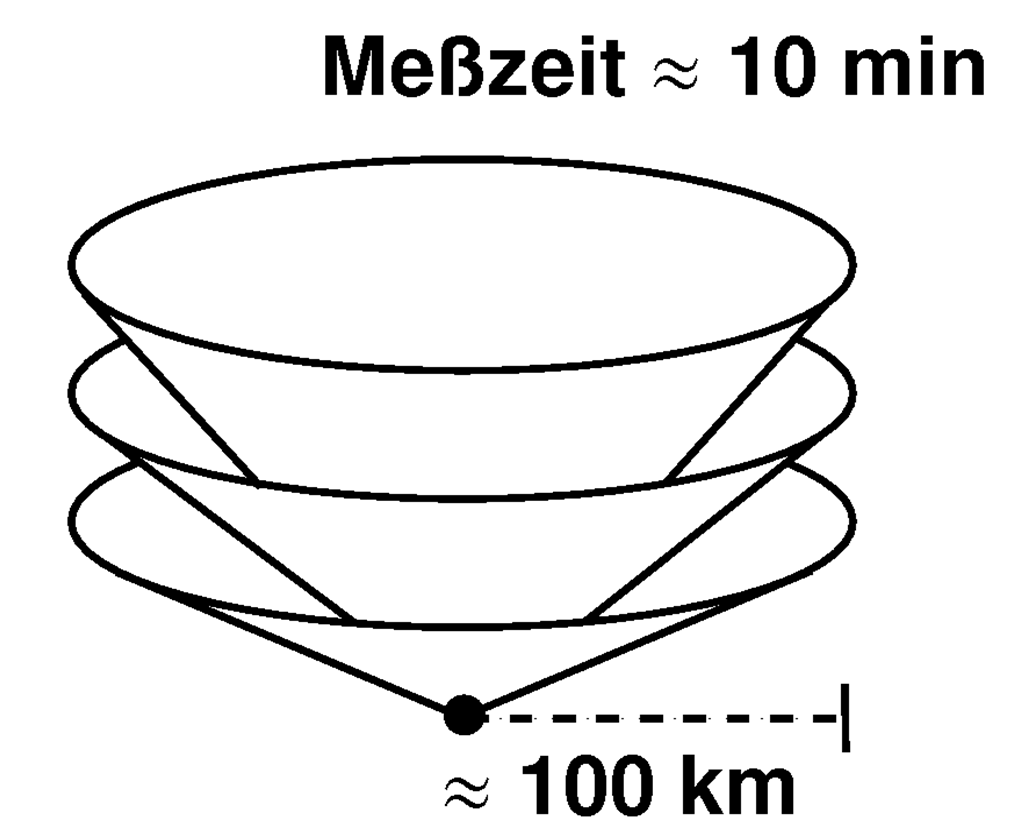
\includegraphics[width=\linewidth*\real{0.32},trim=0 0 100 100,clip=]{radar_principle_vol.png}}
\put(-1.0,9.5){\textcolor{blau}{\rotatebox{30}{\scalebox{\scalfakt}{$\mathbf{Z_{dr}}$}}}}
\put(-1.0,8.0){\textcolor{blau}{\rotatebox{10}{\scalebox{\scalfakt}{$\mathbf{K_{dp}}$}}}}
\put(-1.2,6.5){\textcolor{blau}{\rotatebox{-30}{\scalebox{\scalfakt}{$\mathbf{\rho_{hv}}$}}}}
\put(13.0,7.2){\textcolor{blau}{\rotatebox{-10}{\scalebox{\scalfakt}{$\mathbf{LDR}$}}}}
\put(10.0,6.7){\textcolor{blau}{\rotatebox{20}{\scalebox{\scalfakt}{$\mathbf{A_{dp}}$}}}}
\put(14.0,8.3){\textcolor{blau}{\rotatebox{30}{\scalebox{\scalfakt}{$\mathbf{\Phi_{dp}}$}}}}
\put(0.0,-1.0){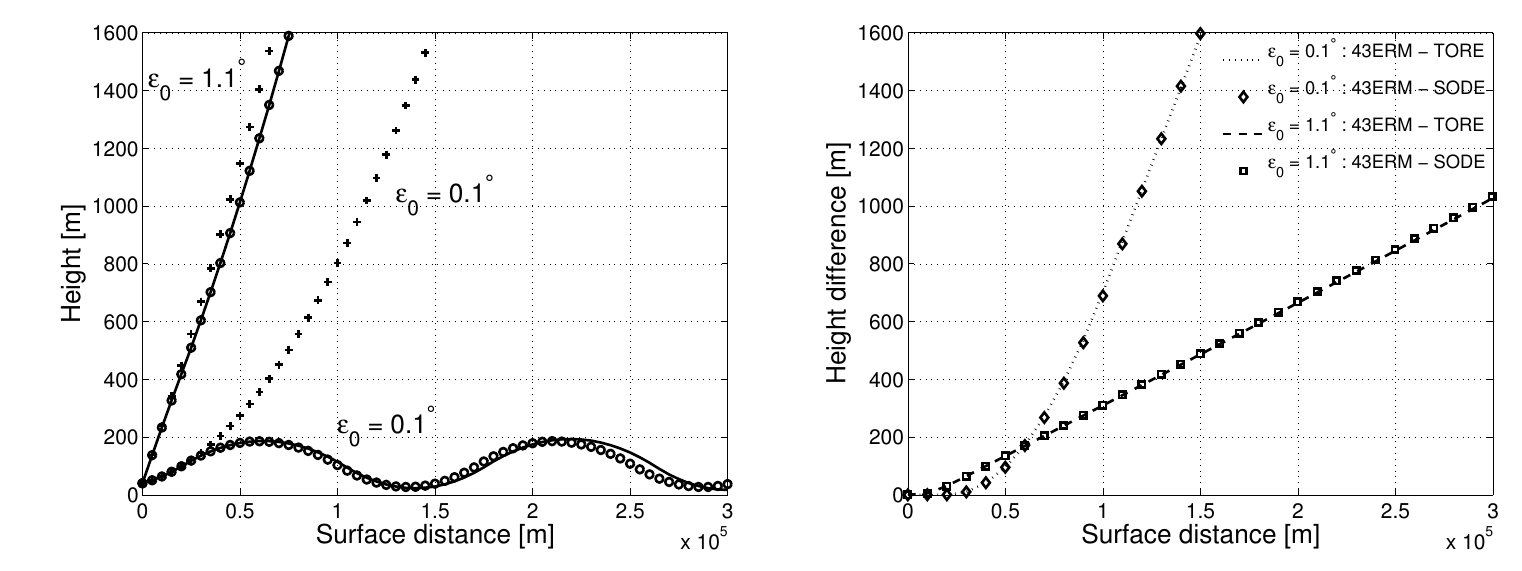
\includegraphics[width=\linewidth*\real{0.85}]{radar_ducting.png}}
\end{picture}

\clearpage

%%% Impressum

\phantom{.}

\vfill

\begin{minipage}{\linewidth}
Created \today\xspace using \LaTeX\xspace and \KOMAScript \\\\\\\\\\
\textbf{\Large Corresponding Author:}\\\\
\textbf{Ulrich Blahak}\\
Deutscher Wetterdienst / German Weather Service (DWD)\\
Frankfurter Str. 135\\
63067 Offenbach
Germany\\[0.5em]
Email: ulrich.blahak@dwd.de \\\\\\

\textbf{\Large Contributors to EMVORADO development:}\\\\
Ulrich Blahak$^{1,2}$, Yuefei Zeng$^{1,2,3}$, Dorit Jerger$^{1}$, Daniel Leuenberger$^{4}$, Axel Seifert$^{1,2}$, Jana Mendrok$^{2}$, Jeffrey Snyder$^{5}$, Jacob Carlin$^{5,6}$, Alberto de Lozar$^{2}$\\\\
$^{1}$ \mbox{Institute for Meteorology and Climate Research (IMK), Karlsruhe Institute of Technology (KIT)}\\
$^{2}$ German Weather Service (DWD), Offenbach, Germany\\
$^{3}$ Meteorological Institute Munich (MIM), Ludwig-Maximilians-University Munich (LMU), Germany\\
$^{4}$ MeteoSwiss, Zurich, Switzerland\\
$^{5}$ National Severe Storms Laboratory (NOAA NSSL), Norman, Oklahoma, USA\\
$^{6}$ Cooperative Institute for Severe and High-Impact Weather Research and Operations, University of Oklahoma, Norman, Oklahoma, USA\\\\\\

\textbf{\Large Where to get this User's Guide?}\\
\begin{itemize}
\item COSMO-Webpage:\\[\itemsep]
  \verb|http://www.cosmo-model.org/content/model/documentation/core/emvorado_userguide_dualpol.pdf|\\[-0.6em]
\item For ICON-NWP users:\\[\itemsep]
  \verb|git@gitlab.dkrz.de:icon/icon-nwp.git| \\[\itemsep]
  \verb|<icon-repo-dir>/externals/emvorado/DOC/TEX/emvorado_userguide.pdf| \\[-0.6em]
\item For EMVORADO standalone offline-framework users:\\[\itemsep]
  \verb|git@gitlab.dkrz.de:dace_projects/emvorado-offline.git| \\[\itemsep]
  \verb|<emvorado-offline-dir>/DOC/TEX/emvorado_userguide.pdf| \\[-0.6em]
\item For EMVORADO core developers:\\[\itemsep]
  \verb|git@gitlab.dkrz.de:dace_projects/emvorado-package.git| \\[\itemsep]
  \verb|<emvorado-package-dir>/DOC/TEX/emvorado_userguide.pdf| \\[-0.6em]
\end{itemize}
\end{minipage}

\thispagestyle{empty}



\cleardoublepage

\tableofcontents
\labelsec{sec:inhalt}

\clearpage

\section{List of changes}
\labelsec{sec:changelog}

\setlength{\lenspeins}{\linewidth*\real{0.1}}
\setlength{\lenspzwei}{\linewidth*\real{0.15}}
\setlength{\lenspdrei}{\linewidth*\real{0.73}-\tabcolsep*\real{4}}

\setlength{\extrarowheight}{0.25\baselineskip}
\begin{longtable}{|p{\lenspeins}|p{\lenspzwei}|p{\lenspdrei}<{\vspace*{\extrarowheight}}|}
\caption*{}\\
\hline
\textbf{Date}           & \textbf{Name}        & \textbf{Change}  \\
\hline
\endfirsthead
\caption*{}\\
\hline
\textbf{Date}           & \textbf{Name}        & \textbf{Change}  \\
\hline
\endhead
%%%%%%%%%%%%%%%%%%%%%%%%%%%%%%%%%%%%%%%%%%%%%%%%%%%%%%%%%%%%%%%%%%%%%%%%%%%%%%
\quetsche{18.9.2019}   & \quetsche{Ulrich Blahak}  &
         \spvierformat{Eliminated namelist switch \paramform{lvoldata_output_supob} from \srcform{/RADARSIM_PARAMS/}. \par
              This switch is not needed, because
              the voldata output of the superobserved fields \srcform{'vrsupobs'}, \srcform{'vrsupsim'},
              \srcform{'zrsupobs'}, and \srcform{'zrsupsim'} can also be triggered via \paramform{voldata_output_list}.\par
              Eliminated from Table~\ref{tab:radarsimparams}.} \\\hline
\quetsche{18.9.2019}   & \quetsche{Ulrich Blahak}  &
         \spvierformat{New namelist parameters \paramform{itype_obserr_vr} and \paramform{thres_dbz_4_obserr_weight}
              in \srcform{/RADARSIM_PARAMS/} to choose the
              method to define the observation error for radial wind which is stored in the feedback files (fof)
              for data assimilation.\par
              Inserted into Table~\ref{tab:radarsimparams}.} \\\hline
\quetsche{19.9.2019}   & \quetsche{Ulrich Blahak}  &
         \spvierformat{New namelist switch \paramform{labort_if_problems_obsfiles} in \srcform{/RADARSIM_PARAMS/}.\par
                       Inserted into Table~\ref{tab:radarsimparams}.} \\\hline
\quetsche{14.10.2019}   & \quetsche{Ulrich Blahak}  &
	 \spvierformat{New namelist parameters  in \srcform{/RADARSIM_PARAMS/} for defining the parameters of the automatic bubbles of the bubble generator.\par
                       Inserted into Table~\ref{tab:radarsimparams}.\par Updated section~\ref{sec:warmbub:impl} accordingly.} \\\hline
\quetsche{02.02.2020}   & \quetsche{Ulrich Blahak}  &
	 \spvierformat{New namelist parameter \paramform{levelidlist_for_composite_glob}  in \srcform{/RADARSIM_PARAMS/} for grib2's levelindex to identify the composites in grib2 records.\par
                       Inserted into Table~\ref{tab:radarsimparams}.\par Updated section~\ref{sec:comporemark}.} \\\hline
\quetsche{14.02.2020}   & \quetsche{Ulrich Blahak}  &
	 \spvierformat{New namelist parameter \paramform{lwrite_ready}  in \srcform{/RADARSIM_PARAMS/} for writing READY-files after each EMVORADO output time step.\par
                       Inserted into Table~\ref{tab:radarsimparams}.\par New according section~\ref{sec:output:ready}.} \\\hline
\quetsche{20.04.2020}   & \quetsche{Ulrich Blahak}  &
         \spvierformat{Eliminated \paramform{thres_dbz_4_obserr_weight}. New namelist parameters \paramform{baseval_obserr_vr}, \paramform{maxval_obserr_vr},
           \paramform{ramp_lowdbz_obserr_vr}, \paramform{ramp_highdbz_obserr_vr}  in \srcform{/RADARSIM_PARAMS/}.\par
                       Inserted into Table~\ref{tab:radarsimparams}.\par According changes in section~\ref{sec:output:format:fof}.} \\\hline
\quetsche{20.07.2020}   & \quetsche{Ulrich Blahak}  &
         \spvierformat{``Warm bubble'' generator now also implemented in ICON. Updated description of corresponding Section~\ref{sec:warmbub} and Subsection~\ref{sec:warmbub:implicon}.} \\\hline
\quetsche{18.09.2020}   & \quetsche{Ulrich Blahak}  &
         \spvierformat{For ICON only: Change default for output grid of composites from COSMO-DE to COSMO-D2. Update Table~\ref{tab:radarsimparams}.} \\\hline
\quetsche{29.03.2021}   & \quetsche{Ulrich Blahak}  &
         \spvierformat{New reader for DWD's flavor of ODIM hdf5 radar observation files. Updated Section~\ref{sec:modero}} \\\hline
\quetsche{29.03.2021}   & \quetsche{Ulrich Blahak}  &
         \spvierformat{New optional output format grib2 for simulated and observed reflectivity volume scans. According updates to Section~\ref{sec:output:format:vol}.} \\\hline
\quetsche{29.03.2021}   & \quetsche{Ulrich Blahak}  &
         \spvierformat{New option for multi-moment multi-volume ouput (\paramform{voldata_format='cdfin-mulmom'} or \paramform{'grib2-mulmom'}). According updates to Section~\ref{sec:output:format:vol}.} \\\hline
\quetsche{29.03.2021}   & \quetsche{Ulrich Blahak}  &
         \spvierformat{New namelist parameter \paramform{dbz_meta_glob} of type \paramform{t_dbzcalc_params}, replacing the previous \paramform{itype_refl_glob} and \paramform{llookup_mie_glob} and offering the possibility to specify global background values of all type components for all radars.} \\\hline
\quetsche{29.03.2021}   & \quetsche{Ulrich Blahak}  &
         \spvierformat{Eliminated \paramform{itype_refl_glob} and \paramform{llookup_mie_glob}} \\\hline
\quetsche{29.03.2021}   & \quetsche{Ulrich Blahak}  &
         \spvierformat{New type components in \paramform{t_dbzcalc_params} of previously hardcoded parameters for EMVORADOs melting sheme. Updates of Table~\ref{tab:dbzmeta} in Section~\ref{sec:nml:dbzmeta}.} \\\hline
\quetsche{29.03.2021}   & \quetsche{Ulrich Blahak}  &
         \spvierformat{Optimized lookup table generation: optimized order of computations with re-cycling of Mie-results and better parallelization. New associated namelist parameters \paramform{itype_mpipar_lookupgen}, \paramform{pe_start_lookupgen} and \paramform{pe_end_lookupgen}} \\\hline
\quetsche{29.03.2021}   & \quetsche{Jana Mendrok}  &
         \spvierformat{\textbf{Polarimetric upgrade of EMVORADO:} introduce polarimetric radar moments in EMVORADO: $Z_{dr}$, $A_{dp}$, $\rho_{hv}$, $K_{dp}$, $\Phi_{dp}$ and $LDR$. New options \paramform{dbz_meta_glob\%itype_refl=5} (T-matrix for spheroidal particles) and \paramform{6} (T-matrix but assuming spherical particles; option for cross-comparison with classical Mie-scattering \paramform{dbz_meta_glob\%itype_refl=1}). No composites and fof-files yet of these new variables. Also no grib2-ouput due to missing shortNames. Processing of polarimetric variables on top of $Z_h$ and $A_h$ is triggered by \paramform{loutdbz=.TRUE.} and \paramform{loutpolstd=.TRUE.} or \paramform{loutpolall=.TRUE.}.} \\\hline
\quetsche{29.03.2021}   & \quetsche{Ulrich Blahak}  &
         \spvierformat{New option for the diagnostic melt fraction as function of particle size and temperature and a new parameter \paramform{dbz_meta_glob\%itype_Dref_fmelt} to select the option (``2'') or use the default scheme (``1''). The new option is somewhat simplified and uses fixed reference diameters in the meltdegree formula instead of some mean PSD size. This greatly enhances the efficiency of polarimetric T-matrix lookup table generation, but also changes the results in the melting layer. Updates of Table~\ref{tab:dbzmeta} in Section~\ref{sec:nml:dbzmeta}.} \\\hline
\quetsche{29.03.2021}   & \quetsche{Ulrich Blahak}  &
         \spvierformat{New possibility to have several output streams (formats, time intervals, file names with flexible file name patterns) for the same volume data. New derived type \paramform{t_voldata_ostream} defining new namelist parameter list \paramform{voldata_ostream(1:noutstreams_max)}} \\\hline
\quetsche{29.03.2021}   & \quetsche{Ulrich Blahak}  &
         \spvierformat{With the introduction of \paramform{voldata_ostream(1:noutstreams_max)}, eliminated the old namelist parameters \paramform{voldata_format}, \paramform{voldata_output_list}, \paramform{cdfin_dt} and \paramform{cdfin_tref}, which are now components of the derived type \paramform{voldata_ostream} and slightly renamed.} \\\hline
\quetsche{29.03.2021}   & \quetsche{Ulrich Blahak}  &
         \spvierformat{New namelist parameter \paramform{ysubdircomp} to explicitly specify the output subdirectory under \paramform{ydirradarout} of composites in grib2. If it starts with a ``/'', it is taken as an absolute path.} \\\hline
\quetsche{29.03.2021}   & \quetsche{Ulrich Blahak}  &
         \spvierformat{New namelist parameter \paramform{composite_file_pattern} to explicitly specify the file pattern of composite files, with the help of (optional) keys.} \\\hline
\quetsche{29.03.2021}   & \quetsche{Ulrich Blahak}  &
         \spvierformat{New namelist parameter \paramform{ysubdirfof} to explicitly specify the output subdirectory under \paramform{ydirradarout} of fof files. If it starts with a ``/'', it is taken as an absolute path.} \\\hline
\quetsche{29.03.2021}   & \quetsche{Ulrich Blahak}  &
         \spvierformat{New namelist parameter \paramform{ydir_ready_write} to explicitly specify the output directory for READY files.} \\\hline
\quetsche{29.03.2021}   & \quetsche{Ulrich Blahak}  &
         \spvierformat{New namelist parameter \paramform{ready_file_pattern} to explicitly specify the file pattern of READY files, with the help of (optional) keys.} \\\hline
\quetsche{15.04.2021}   & \quetsche{Ulrich Blahak}  &
         \spvierformat{New namelist parameter \paramform{llookup_interp_mode_dualpol} to switch to a consistent interpolation technique for table lookup among all polarimetric moments (cubic interpolation of linear values). Avoids interpolation artifacts, e.g., values of $\rho_{hv}>1$.} \\\hline
\quetsche{15.04.2021}   & \quetsche{Ulrich Blahak}  &
         \spvierformat{New namelist parameter \paramform{lcalc_dbz_on_radarbins} for new option to switch the order of interpolating model state variables to radarbins and computing polarimetric moments. If \srcform{.TRUE.}, first interpolate the model state and then compute radar moments. Only implemented for 4/3-earth beam propagation (\paramform{lonline=.FALSE.}).} \\\hline
\quetsche{11.08.2021}   & \quetsche{Ulrich Blahak}  &
         \spvierformat{New type component \paramform{voldata_ostream\%grib2_packingtype} of namelist parameter \paramform{voldata_ostream} to explicitly define the grib2 packing type. Up to now, the packing type \paramform{grid_ccsds} was hardcoded.} \\\hline
\quetsche{04.12.2021}   & \quetsche{Ulrich Blahak}  &
         \spvierformat{In obs data mode (\paramform{lreadmeta_from_netcdf=.TRUE.}), new possibility to add further stations in the namelist-driven re-definition step of station metadata. Up to now, it was only possible to change metadata of existing stations in obs files. To enable correct setting of obs times, set the new \paramform{rs_meta($i$)\%lobstimes_ovwrt_recalc=.TRUE.} for every new station $i$.} \\\hline
\quetsche{04.12.2021}   & \quetsche{Ulrich Blahak}  &
         \spvierformat{In obs data mode, enable to extend/change the obs times for stations present in obs files. For this, new type component \paramform{rs_meta($i$)\%lobstimes_ovwrt_recalc} (logical) of namelist parameter \paramform{rs_meta} to trigger re-calculation of the series of output times for station $i$ where \paramform{rs_meta\%dt_obs} and/or \paramform{rs_meta\%nobs_times} have been changed by namelist after obs metadata reading. If no obs are available for a certain time, the production of obs composites and the bubble generator are skipped.} \\\hline
\quetsche{04.03.2022}   & \quetsche{Ulrich Blahak}  &
         \spvierformat{In obs data mode, enable to process OPERA hdf5 files (file names starting with \paramform{T_PA}) of Switzerland and Belgium.} \\\hline
\quetsche{04.03.2022}   & \quetsche{Ulrich Blahak}  &
         \spvierformat{In obs data mode, enable to switch off the writing of radial winds and reflectivity to the feedback files for single radar stations. For this, new type components \paramform{rs_meta($i$)\%lvrad_to_fdbk} and \paramform{rs_meta($i$)\%ldbzh_to_fdbk} (logicals) of namelist parameter \paramform{rs_meta}. And because for some countries the Nyquist velocity alternates between different elevations and/or times, radial winds might or might not be usable for assimilation. The new type component \paramform{rs_meta($i$)\%vnyq_min_for_vr_active_fdbk} allows to set a threshold Nyquist velocity above which radial winds are set \paramform{active} in feedback files. Otherwise \paramform{passive}.} \\\hline
\quetsche{19.03.2022}   & \quetsche{Ulrich Blahak}  &
         \spvierformat{In obs data mode, enable to process OPERA hdf5 files of France, Denmark, Netherlands, Poland, Czech Republik and Germany.} \\\hline
\quetsche{03.08.2022}   & \quetsche{Ulrich Blahak}  &
         \spvierformat{Allow possibility to have different composite grids for the warm bubble generator and the ``normal'' composite output. New namelist parameters \paramform{comp_meta_bub}, \paramform{lcomposite_output_bub}, and \paramform{composite_file_pattern_bub}.} \\\hline
\quetsche{11.09.2022}   & \quetsche{Ulrich Blahak}  &
\spvierformat{In obs data mode, enable to process OPERA hdf5 files of Slovakia.} \\\hline
\quetsche{23.11.2022}   & \quetsche{Jana Mendrok}  &
\spvierformat{New namelist parameters in \paramform{dbz_meta} that allow specification of hydrometeor shape and orientation for dual polarization calculations. Inserted in Table~\ref{tab:dbzmeta}.} \\\hline
\quetsche{29.11.2022}   & \quetsche{Ulrich Blahak}  &
\spvierformat{Renamed type \paramform{dbzcalc_params} to \paramform{t_dbzcalc_params}.} \\\hline
\quetsche{07.12.2022}   & \quetsche{Ulrich Blahak}  &
\spvierformat{Increased \paramform{nradsta_max} from 80 to 120. Decreased \paramform{ndoms_max} from 5 to 3.} \\\hline
\quetsche{10.4.2023}   & \quetsche{Ulrich Blahak}  &
\spvierformat{New format for namelist parameters \paramform{rs_meta\%dt_obs}, \paramform{rs_meta\%dt_obs_voldata}, \paramform{rs_meta\%dt_obs_fdbk},
  \paramform{dt_obs_voldata_glob} and \paramform{dt_obs_fdbk_glob}. Instead of specifying just the time increment for the time lists and
  implying that the times run from model start time to end time, now a time triple has to be given: \paramform{from-time, to-time, increment}.
  However, for backwards compatibility, one can also give only one value in the namelist, which is interpreted as the increment and automatically shifted to the correct position in the triplet. \paramform{from-time} and \paramform{to-time} are set to -999.9 in this case. If \paramform{from-time} is less than -900, the series of times starts (approximately) at model init time and is synchronized to time 0.0\,s. If \paramform{from-time} is larger than -900, it is interpreted as the exact start time of the series and is not synchronized to time 0.0\,s.} \\\hline
\quetsche{07.08.2023}   & \quetsche{Ulrich Blahak}  &
\spvierformat{Increased \paramform{nradsta_max} from 120 to 140.} \\\hline
\quetsche{07.08.2023}   & \quetsche{Ulrich Blahak}  &
\spvierformat{KIT hdf5 radar observation files can now be processed: KIT C-band radar Karlsruhe with pseudo WMO-ID 20001 and non-standard hdf5-files (see Section~\ref{sec:modero}) with an own special reader.
  KIT-Cube X-band radar with pseudo WMO-ID 10000 and ODIM-conforming hdf5-files, using the existing OPERA reader (see Section~\ref{sec:modero}).} \\\hline
\quetsche{24.08.2023}   & \quetsche{Ulrich Blahak}  &
\spvierformat{New switch \paramform{dbz_meta\%ldynamic_wetgrowth_gh} (default \srcform{.FALSE.})\par If \srcform{.TRUE.}, switch on new option for dynamic determination of \paramform{dbz_meta\%Tmeltbegin_g/h} and \paramform{dbz_meta\%meltdegTmin_g/h} for graupel and hail categories in each grid column, according to the actually present supercooled liquid in relation to the actual mean particle sizes and the wet growth diameters.
This improves simulated radar moments in and above the melting layer. More informations in Section~\ref{sec:nml:dbzmeta}.} \\\hline
\quetsche{30.08.2023}   & \quetsche{Ulrich Blahak}  &
\spvierformat{Changed the default $T$-thresholds related to the freezing point of water from .16 to .15 for consistency to ICON microphysics. This changes all radar moments slightly, but not significantly.} \\\hline
\quetsche{21.05.2024}   & \quetsche{Ulrich Blahak}  &
\spvierformat{New namelist parameters \paramform{dbz_meta($i$)\%ext_tune_fac_pure} and \paramform{dbz_meta($i$)\%ext_tune_fac_melt} (logical) to tune the attenuation coefficients. This enables to ``adjust'' the forward simulation to observations where the attenuation has been partly/conservatively corrected. Updates of Table~\ref{tab:dbzmeta} in Section~\ref{sec:nml:dbzmeta}.} \\\hline
\quetsche{24.9.2024}   & \quetsche{Ulrich Blahak}  &
         \spvierformat{New namelist switch \paramform{labort_if_problems_gribout} in \srcform{/RADARSIM_PARAMS/}.\par
                       Inserted into Table~\ref{tab:radarsimparams}.} \\\hline
%
%
%%%%%%%%%%%%%%%%%%%%%%%%%%%%%%%%%%%%%%%%%%%%%%%%%%%%%%%%%%%%%%%%%%%%%%%%%%%%%%
%\quetsche{18.9.2019}   & \quetsche{Ulrich Blahak}  &
%        \spvierformat{        } \\\hline
\end{longtable}



\clearpage

\section{Introduction}
\labelsec{sec:intro}


\subsection{Basic information}

\labelsec{sec:intro:basic}

The \textbf{E}fficient \textbf{M}odular \textbf{VOLume} \textbf{RAD}ar forward \textbf{O}perator \textbf{EMVORADO} computes
synthetic radar volume scan observations of
\begin{itemize}
\item[-] radial wind (m\,s$^{-1}$)
\item[-] horizontally polarized radar reflectivity $Z_h$ (dBZ)
\item[-] differential reflectivity $Z_{dr}$ (dB)
sd\item[-] horizontal attenuation coefficient $A_h$ (dB/km)
\item[-] specific differential phase shift $K_{dp}$ (\grad/km)
\item[-] total differential phase shift $\Phi_{dp}$ (\grad)
\item[-] cross-correllation coefficient $\rho_{hv}$
\item[-] linear depolarization ratio $LDR$
\item[-] differential attenuation $A_{dp}$ (db/km)
\end{itemize}
on the basis of the simulated prognostic atmospheric fields of NWP-models for a given set of radar stations. 
From a scientific point of view it is documented to a large degree (Mie- and Rayleigh options, beam bending options, beam smoothing options) in \citeP{blahak2016a}, \citeP{zeng2013}, \citeP{jerger2014}, \citeP{zeng2014} and \citeP{zeng2016a}.
The listed polarization parameters have recently been added and are based on the works of \citeP{ryzhkov2001} and  \citeP{ryzhkov2011}, approximating all hydrometeors
as one- or two-layered oblate spheroids and employing the T-matrix method to compute scattering properties. Here it is assumed that the so-called
``backscatter-rule'' as an approximation of the scattering-properties as funcion of the particle orientation relative to the incoming wave holds,
which requires that the particle size is not too large compared to the wavelenght (\citeNPK{ryzhkov2001}) and that the elevation angle is not too steep (\citeNPK{ryzhkov2011}). It is planned to relax this condition in the
near future.

Radar data can be output for different purposes and in different formats. The ``raw'' volume data are useful for
model verification or a postprocessing by methods/software from the radar community, such
as compositing or the detection of simulated convective ``cell objects''. EMVORADO is able to
produce and output it's own reflectivity ($Z_h$) composites. It can also process observed volume scans alongside the simulated
data to produce so-called ``feedback'' files as input for DWD's KENDA data assimilation system, which contain
pairs of observed and simulated reflectivities. For this, the computation spacially averaged super-observations at regular spatial intervals is possible as an option.
From the composites of observed and simulated reflectivites EMVORADO offers the option to detect missing convective cells
in the hosting model and to provide informations for automatic artificial convection triggers (``warm bubble generator'')
to spin up missing convective cells in the model.

Use of the forward operator can be switched on by the top level namelist parameter \srcform{luse_radarfwo} in one of the
top-level namelist in the hosting model (COSMO: \srcform{/RUNCTL/}; ICON: \srcform{/run_nml/}),
provided that the model has been compiled with a number of additional pre-processor switches, cf. Section~\ref{sec:compil}.

EMVORADO provides options for different degrees of ``physical'' approximation for certain scattering- and radar measurement
processes, to provide the possibility to find the ``best'' compromise between
necessary physical accuracy and computational efficiency for the user's respective application.
These options are described in detail in \citeP{zeng2016a} and can be configured in
an operator-specific namelist \srcform{/RADARSIM_PARAMS/} (COSMO: file \srcform{INPUT_RADARSIM}, ICON: file \srcform{NAMELIST_EMVORADO}).
The polarimetric parameters have been integrated into these processes accordingly.

The present document provides an overview on the operator and its different
application modes (Section~\ref{sec:modes}), its different namelists
(operator-specific and hosting model) in Section~\ref{sec:nml},
data formats for radar observation input (Section~\ref{sec:modero})
and operator output (Section~\ref{sec:output}), code compilation (Section~\ref{sec:compil}),
as well as general aspects of operator development (Section~\ref{sec:devel}), including implementation
into hosting models in general (Section~\ref{sec:impl}) and in COSMO (Section~\ref{sec:implcosmo}) and ICON (Section~\ref{sec:implicon}).


Concerning the code, EMVORADO is written in Fortran~2003. Most modules are not specific
to a particular NWP-model but can in principle be coupled to any NWP-model (``core'' modules).
To connect the model world to the EMVORADO core, there is one model-specific
module \srcform{radar_interface.f90} which, for example, exchanges time informations, feeds the model state variables to EMVORADO,
provides interpolation routines (model grid $\Longrightarrow$ geographic coordinates $\Longrightarrow$ radar bins),
exchanges MPI communicators and -data types, and so on. Concerning the coupling to the particle- and size distribution shapes of specific bulk cloud microphyscis schemes,
EMVORADO currently implements the 1-moment- and 2-moment bulk microphysics of COSMO and ICON, but in a rather generic way, so that it might be
possible to connect also other microphysics schemes.
More details on the implementation
and coupling can be found in Section~\ref{sec:impl}.

There is also a so-called ``offline'' framework (a simple but fully MPI-parallel stand-alone wrapper around the core), which reads
one timestep of model fields from disk and feeds it to the core. The parallelization strategy of the wrapper is derived from
that of the COSMO-model and makes use of parts of the COSMO code. For the core, it ``fakes'' the COSMO environment (data structures,
timers, domain decomposition, rotated lat-lon grid) and expects a COSMO-like rotated lat-lon grid for the model state variables on input.
Because ICON is able to interpolate it's output variables to such a grid for output, it is possible to use the offline framework also for ICON input data.

EMVORADO is designed to handle entire networks of radar stations and allows different
wavelengths, scan strategies and output times for different stations. These and the
other relevant station metadata (geographic location, height, etc.) may be specified
explicitly in the \srcform{/RADARSIM_PARAMS/} namelist or taken from actual
observation files (if available). With the namelist-based station definition method,
even idealized simulations with COSMO and virtual radar stations are possible
(e.g. OSSE studies for scientific questions in data assimilation).
As mentioned above, these different simulation modes are described in more detail in Sections~\ref{sec:modes}.

Internally in EMVORADO one radar station is defined as the combination of a WMO station ID and a certain scan strategy (= set of elevation angles).
This means for example, that if the same station conducts two alternating scan strategies, these are internally handled as two different radar stations.
In that sense, DWD's horizon-following ``precipitation scans'' which alternate with volume scans are handled as different radar stations.


With regards to its contents, the operator for $Z_h$, $A_h$ and the polarization parameters is composed of two steps.

Step~1: Computation of unattenuated $Z_h$, $A_h$ (optional for Mie- and T-matrix scattering, see below) and polarization parameters
on the model grid based on the simulated hydrometeor fields (depending on the chosen
microphysics scheme) as described in \citeP{blahak2016a} and \citeP{zeng2016a} for $Z_h$ and $A_h$ and \citeP{ryzhkov2011} for the polarization parameters.
There are 5 general options. The first is Mie-scattering, the second and third are two
variants of the so-called Rayleigh approximation for particles small compared to the wavelength, the fourth is T-matrix for oblate spheroids, and the fifth is T-matrix for spheres.
The main difference of the two Rayleigh options is the treatment of melting hydrometeors.

Step~2: Interpolation/aggregation of the $Z_h$, $A_h$ and polarization parameters to the
radar bins (polar coordinates range, azimut, elevation) with an option for explicit ray tracing, optional iterative computation
of attenuation effects along each ray (only possible for Mie- or T-matrix options), starting at the radar station, and output of volume
scan data to files. Step~1 depends on the radar wavelength (also slightly in the first of the two Rayleigh options), and because different
radar stations are allowed to have different wavelengths, it is repeated for each single
radar station.

However, if consecutive simulated radars have the same wavelength and other scattering-theory-specific
settings, some efficiency is gained
by just re-using the computed radar parameters from the last radar instead of repeating the computation.

This procedure is the traditional way of computing $Z_h$ and $A_h$ in EMVORAO, which can be very efficient for large radar networks, because it
reduces the amount of $Z_h$ and $A_h$ computations to a minimum. However, consistency of the different parameters with respect to the implicit particle size distribution is not guaranteed,
if the interpolation to radar bins in step~2 is of type linear (COSMO).
For this, a new option has been implemented to interchange the order of interpolation and computation of parameters:
first the model state variables (hydrometeors, temperature $T$, pressure $p$) are interpolated to the radar bins before computing the scattering parameters on the radar bins.
This ensures consistency among the parameters, because they are based on the same interpolated hydrometeor properties. The modified steps
are as follows, if the namelist parameter \paramform{lcalc_dbz_on_radarbins} is set .TRUE.:

Modified step~1: Interpolation of model state variables to the positions of the radar bins, optionally after explicit ray tracing, then computation of
unattenuated $Z_h$, $A_h$ (optional for Mie- and T-matrix scattering, see below) and polarization parameters
on the radar bins based on the interpolated hydrometeor fields and $T$. In this way, the computation of the radar parameters
has to be triggered for the radar bins of each radar station individually and no re-use of computed values from a previous computation is possible.
Depending on the number of model grid points and the number of radar stations and their scan strategy, this might be computationally more cheap or more expensive.
But in this way it is naturally to take the local elevation angle correctly into account, which might become relevant at higher elevations
for oblate spheroids.

Modified step~2: Optional averaging of the $Z_h$, $A_h$ and polarization parameters over the effective beam weighting function, optional iterative computation
of attenuation effects along each ray (only possible for Mie- or T-matrix options), starting at the radar station, and output of volume
scan data to files.

Note that this is not necessary for ICON, because in that case the interpolation method in step~2 is Nearest Neighbour, which preserves the consistency.
This method leads however to coarser radar signatures in simulated data and has been chosen for technical reasons due to the unstructured nature of the triangular ICON model grid. Other interpolation methods
would have been computationally much more expensive because there are no regulatrities which can be exploited to efficiently find the
surrounding grid point neighbourhood for interpolation.

The operator for radial wind is similar, but if some grid point calculations (step~1) are necessary or not
depends on the physical configuration. Step~1 is only necessary, if the reflectivity weighted terminal fall velocity
of hydrometeors is taken into account in the radial winds. If yes, this velocity is derived along the
lines of the grid point values from the model hydrometeor fields. The reflectivity for weighting the 
fall velocity is however always according to the Rayleigh approximation, see \citeP{zeng2016a}.
Step~2: Interpolate/aggregate U, V, W to the radar bin positions (polar radar coordinates
range, azimut and elevation), compute the radial wind as described in \citeP{zeng2016a} and
output volume scan data to files. This is similar to step~2 for the reflectivty.


\subsection{Remark about online domain nesting capabilities}

\labelsec{sec:intro:idom}

For models like ICON with the capability for online nesting runs with multiple model domains, EMVORADO
is ready to be applied independently to the different model domains.
In this case, the namelist parameter \srcform{luse_radarfwo} is a list of switches for each
model domain. Each domain for which \srcform{luse_radarfwo($k$)=.TRUE.} is called ``radar-active'' in the following.

An own \srcform{/RADARSIM_PARAMS/} for each radar-active model domain is required.
There is a mandatory namelist parameter \srcform{dom} (domain number, integer) to indicate
which namelist belongs to which model domain. In COSMO we always have to set \srcform{dom=1}.
If this parameter is missing in the \srcform{/RADARSIM_PARAMS/} namelist, the run will stop with an
appropriate error message.


\subsection{Parallelization}

\labelsec{sec:intro:parallel}

The operator code is parallelized as described in \citeP{zeng2016a}. The details of the
parallelization strategy depend on the optionally chosen degree of physical approximation of the radar
measurement process, in particular if the beam propagation is modeled by the simple
climatological ``4/3-earth-model'' (sufficient for most applications) or by an actual
ray-tracing method based on the simulated actual field of the air refractive index.
More details about the underlying physics can be found in \citeP{zeng2014}. 


Technically, the step~2 for radial wind, $Z_h$ and polarization parameters is divided into two sub-parts,
related to the parallelization strategy. Each compute-PE contains a subset of the radar bins
of each station, depending on the horizontal domain decomposition (number of compute PEs in $X$- and $Y$-direction)
and the position and scan strategies of the radar stations. The polar radar bins of
one station might or might not be spread over several compute-PEs. In the first sub-part, 
the interpolation/aggregation of model grid point values to the subset of radar bins is done by
each compute-PE separately in parallel. In the second sub-part, the subsets on different PEs for
each station are collected on dedicated output-PEs, one for each station and sorted into full
3D volume scan arrays (range, azimut, elevation). At this point, additional computations
which require continuous and sorted data (e.g., optional iterative attenuation computation along each ray,
super-observations for the data assimilation feedback files, radar composites of observed and simulated reflectivity) can
be perfomed, before the data are output into files.

Normally these output processors are among the compute processors, i.e., if the hosting model runs on 100~PEs and there are 17 radar stations to simulate,
the first 17 compute PEs will do the output for the 17 stations in parallel. There can be
however less processors than stations, in which case each processor does output for several stations one after another
in a round-robin fashion. Even single-processor-runs are possible.

This ``synchroneous'' strategy has however the effect that the non-output PEs have to
wait for the output PEs to finish their computations and data output before the COSMO-model
can continue with the next model time step. This leads to a more or less strong
load imbalance among the compute-PEs, because not only the output can be costly, but also the
abovementioned additional computations before the actual output.

Therefore, there is also an asynchroneous mode in the EMVORADO code where the radar output processors can
be extra PEs dedicated exclusively to radar data IO, similar to the already existing asynchroneous
grib output of the COSMO-model. This mode can be activated by simply specifying the desired extra number
of PEs as the namelist parameter \srcform{nprocio_radar} in COSMO (namelist \srcform{/RUNCTL/}) or \srcform{num_io_procs_radar} in ICON (namelist \srcform{/parallel_nml/}).
Here, the compute-PEs can continue with their model time step integration while
the output-PEs are doing their output tasks in parallel.
If more than one model domain is radar-active, the asynchroneous radar-IO-PE's are automatically sub-divided
over the number of radar-active domains.


From a technical standpoint, the ray-tracing method requires an intermediate parallelization step. The atmospheric
refractive index $n$ (function of $T$, $p$ and $q_v$), the wind components and the grid point reflectivity
are interpolated to so-called azimuthal slices. These are vertical 2D slices extending
radially outwards from each radar station for all discrete azimut angles of the radar scan strategy. For the ray tracing,
the complete data of one azimutal slice have to be present on one processor, which is achieved in a special MPI communication. Moreover,
the set of slices from all stations is evenly distributed over the compute-PEs to do the ray tracing for the radar bin heights as function of range in parallel and to interpolate the
wind components and reflectivity to these bin positions. 

If the so-called beam function smoothing option is enabled, which is, for each radar bin value, a weighted integral averaging procedure using
a Gaussian kernel over some neighborhood volume, the radar bin values in sub-part~1 of step~2 are in fact the values at
some auxiliary Gauss-Legendre-nodes around each radar bin center, but otherwise the same parallelization strategy is employed.
The actual integral averaging is done in sub-part~2 on the output-PEs, after the optional attenuation computation.


\subsection{Options for scattering computations of different physical accuracy and efficiency}
\labelsec{sec:intro:dbz}

The choice of the reflectivity and dual polarimetric parameter computation method (cf. Section ~\ref{sec:intro:basic} above) is governed by a namelist parameter \srcform{itype_refl} that appears
in different contexts, also as derived type component, in radar-related namelists.
A number of sub-parameters govern some intrinsic details of the computation method, mostly for the Mie- and T-matrix options.
An in-depth discussion and documentation, especially with regards to melting hydrometeors (radar ``bright band'') can be found in 
Chapter~6 of \citeP{blahak2016a}. The parameters described therein appear below in Sections~\ref{sec:nml:dbzmeta} and~\ref{sec:nml:gpout}.

For Mie- and T-matrix scattering, the use of efficient lookup tables
replacing the full expensive computations is implemented and strongly advised (cf. Section~\ref{sec:intro:lookup} below). With this,
Mie- and T-matrix scattering become computationally as cheap as the Rayleigh options. The namelist switch \srcform{llookup_mie=.TRUE.} activates
the use of lookup tables and also appears in different contexts in namelists and derived types. The tables themselves are autogenerated by EMVORADO
if necessary; the full Mie- and T-matrix routines are included in the code.

A ``normal'' user should only choose the radar wavelength and the overall type of reflectivity computation.
The following options are provided in EMVORADO:
\begin{itemize}
\item \srcform{itype_refl = 1}: Mie-scattering option assuming spherical particles for all hydrometeors. With this, $Z_h$ and optionally $A_h$ are simulated.
  Particle sizes are allowed to be larger than the wavelength, but all particles are assumed spherical. The dual polarization parameters are simply set to their ``spherical'' neutral values.
  A detailed treatment of melting hydrometeors (cf. \citeNPK{blahak2016a}, Sections~4, 5, 8) allows for halfway realistic bright bands, at the same time allowing to explore
  the wide range of uncertainty by choosing many options for the refractive index of ice/water/air mixture particles (so-called Effective Medium
  approximations or EMA's).

  If switching on the lookup table option (\srcform{llookup_mie=.TRUE.}), very good efficiency is achieved, because the (autgenerated) tables directly relate reflectivity to the prognostic
  hydrometeor moments and temperature, and, concerning efficiency, there is no reason to choose the below Rayleigh approximations any more. 
\item \srcform{itype_refl = 3}: Rayleigh-scattering approximation using the Oguchi-formulation of the effective refractive index of melting hydrometeors as described in \citeP{blahak2016a}, Section~6.2. Only $Z_h$ is simulated. The approximation contains an
  analytic formulation for melting hydrometeors which leads to a systematic underestimation of bright bands. $Z_h$ is overestimated, if the particle sizes are comparable or larger than the radar wavelength.
\item \srcform{itype_refl = 4}: ``Old'' standard method for reflectivity computation from \srcform{pp_utilities.f90}. It is also a Rayleigh-scattering approximation for $Z_h$ only, but it contains only a much more simplistic treatment
  of melting hydrometeors, leading to unrealistic and ``jumpy'' bright bands. $Z_h$ is also overestimated, if the particle sizes are comparable or larger than the radar wavelength.
\item \srcform{itype_refl = 5}: Similar to \paramform{itype_refl=1} but replacing Mie by T-matrix calculations assuming oblate spheroids following \citeP{ryzhkov2001,ryzhkov2011}. EMA's and melting model are the same as for Mie.
  With this, $Z_h$, $Z_{dr}$, $A_h$, $\rho_{hv}$, $K_{dp}$, $\Phi_{dp}$, $LDR$, and $A_{dp}$ are simulated.
  Further necessary assumptions on size-dependend particle asymetry and hydrometeor-dependend canting angle distributions are largely taken from \citeP{ryzhkov2011} but subject to future changes.
\item \srcform{itype_refl = 6}: Similar to \paramform{itype_refl=5} but replacing oblate spheroids by ordinary spheres. This option can be used to cross-check T-matrix codes with Mie in the spherical limit.
\end{itemize}
For the other parameters in Table~\ref{tab:dbzmeta}, the defaults are ``reasonable'' and with respect to melting particles, they lead to an ``intermediately strong'' bright band.
To attain ``stronger'' or ``weaker'' bright bands (the uncertainty range is ~10~dB!), an experienced user might change the parameters for the EMA's based on
the detailed informations and extensive figures given in \citeP{blahak2016a}.

Note that the option \srcform{itype_refl = 2} which has been described in Section~6.3 of \citeP{blahak2016a}, has been eliminated from the code in the meantime.
It was similar to option~1 with respect to the EMA's for melting particles but replaced the exact Mie-backscattering coefficients by the ``$D^6$'' Rayleigh-approximation.
This saved computing time with respect to the original backscattering coefficient calculation of single particles, but still required numerical integration over the size distributions to
compute the reflectivity. With the advent of the Mie-lookup tables, this option did no longer provide any substantial computational advantage and at the same time
its application was restricted to particles small compared to the wavelength and neglected attenuation.


\subsection{Enhancement of traditional grid point output of unattenuated $Z_h$ (COSMO only)}

\labelsec{sec:intro:gpout}

With the coupling of EMVORADO to COSMO, the traditional output of (unattenuated) $Z_h$ on the model grid (\srcform{/GRIBOUT/} namelists), namely the fields
\srcform{DBZ} (\srcform{yvarml}, \srcform{yvarpl}, \srcform{yvarzl}), \srcform{DBZ_850} (\srcform{yvarml}), \srcform{DBZ_CMAX} (\srcform{yvarml}) and \srcform{DBZ_CTMAX} (\srcform{yvarml}),
can now be computed optionally by the EMVORADO methods of Mie-/T-matrix scattering and Rayleigh-Oguchi-approximation as in (unmodified) step~1 of EMVORADO. \textbf{No polarization parameters at the moment!}
The computation method for these values can be
configured separately in the \srcform{/GRIBOUT/} namelist(s) by a set of new namelist parameters. The previous method from \srcform{pp_utilities.f90} is still available as an option.
Internally, these grid point values are independent of the ones of EMVORADO step~1 which go into it's step~2, because of independent calls to the
respective functions.
But again, if the same reflectivity computation settings are chosen here as in
step~1 (wavelength and other parameters), efficiency is gained by re-using reflectivity values from the last subroutine call instead of new computations.

For ICON, a similar mechanism for grid point reflectivity is planned, but it is not implemented yet.

\subsection{Lookup tables for Mie- and T-matrix scattering options}

\labelsec{sec:intro:lookup}

Concerning the Mie- and T-matrix options for $Z_h$, $A_h$ and polarization parameters, considerable speedup can be gained by using lookup tables (one table for
each model hydrometeor category plus melting hydrometeors). T-matrix computations are even more (much more!) demanding than Mie-computations and lookup tables are key
for any larger-scale operational application of EMVORADO in data assimilation or model verification.
Therefore this option is strongly recommended and can be chosen by namelist switches, both for step~1 computations in EMVORADO and
for the output of grid point reflectivities. It leads to about the same runtime as the Rayleigh-
approximations and enables to take attenuation into account for the volume scans in EMVORADO.
There is an automated mechanism to handle the generation of lookup-tables (the full Mie- and T-matrix codes are part of EMVORADO), storage in fortran binary files and re-using existing tables.
Once the option is chosen, things happen automatically and thread-safe. 

For the COSMO- and ICON-models and their bulk cloud microphysical schemes with pre-scribed mass-size-relations, particle size distribution (PSD) shapes and other particle-related assumptions,
the simulated radar moments like  $Z_h$, $Z_{dr}$, $A_h$, $K_{dp}$ and other polarization parameters
depend uniquely on the prognostic hydrometeor moments and temperature $T$. The temperature dependency arises due to the temperature-dependend melting scheme in EMVORADO
and to a lesser degree due to the temperature dependency of the refractive indices for ice and water. EMVORADO's lookup tables tabulate, separately for each hydrometeor type and dry/melting state, the radar moments at regularly spaced
intervals (table nodes) of the hydrometeor variables and temperature. Once pre-computed, the radar moments for actual model states are computed by fast interpolation of the tabulated values and summed up over all hydrometeor types.
The tables are as low dimensional as possible. In the simplest case of a one-moment scheme there are two dimensions, mass density and $T$. But even for the two-moment scheme of COSMO and ICON and a melting hydrometeor type there are only 3 dimensions,
namely the ratio of mass- to number density (mean size), $T$ and a proxy for the melting state.

The names of the lookup table files are unique and consist of the hydrometeor type names, the scattering theory name, an identifier for the cloud microphysics scheme with which they are consistent,
a "magic number" (10 digit signed integer) which is a unique hash-value representing the exact configuration parameters
of the reflectivity/scattering calculation (c.f. Sections~\ref{sec:nml:dbzmeta} and~\ref{sec:nml:gpout}), and the internal version number. Examples of files containing Mie- and T-matrix tables for dry graupel are
\begin{center}
  \verb|radar_tmatrixtab_2mom_drygraupel_1545262779_version009.bin|\\[0.3em]
  \verb|radar_mietab_2mom_drygraupel_0583900982_version009.bin|
\end{center}
The hash value depens uniqely on  the configuration parameters for the reflectivity/polarization calculation.
At simulation start, EMVORADO checks for each hydrometeor type if a table file with the respective hash-value is present on disk. If yes, the existing table is read from disk and used.
If not, the generation of the table is triggered, which takes some additional runtime, and the result is stored in a new table file on disk for subsequent model runs.

The user can specify the directories where to write and read these files via namelist (\srcform{ydir_mielookup_read} and \srcform{ydir_mielookup_write}).
At each model start it is checked which different reflectivity configurations (wavelength, details of melting hydrometeors,
etc.) are needed among all radar stations and grid point output streams (COSMO only at the moment) for this model run, and based on
the respective hash values the respective files are searched in the given read-directory. If the file is found,
it is read from disk and re-used. If it does not exist, the respective table is computed and the
file is created in the write-directory. Ideally the read- and write-directories should be defined equal and non-temporary,
in which case no manual interaction (copying table files around) is necessary.

If the read- and write-directories are the same and are permanent, the user does not have to care about. This
should be the preferred way for the ``normal'' user. However, in some operational environments it is
desired for technical reasons to limit the direct model output exclusively to temporary directories and move it afterwards
to where it should be stored permanently. This requires the possibility to read lookup tables
from a different directory than where they are written to, but needs manual copying of newly created tables to
the read-directory.

Motivated by the very long time it may take to generate T-matrix tables, the table generation is parallelized (MPI) over the processors of the model run.
The way how this task is parallelized in detail can be configured by the namelist switches \srcform{itype_mpipar_lookupgen}, \srcform{pe_start_lookupgen} and \srcform{pe_end_lookupgen}.
Their defaults are a reasonable choice for most platforms.


\subsection{Output of radar composites}

\labelsec{sec:intro:compo}

2D composites of simulated and observed $Z_h$ (useful e.g. for spatial model verification in dBZ-space or for the detection of missing cells for automatic warm bubbles, see Sections~\ref{sec:comporemark} and~\ref{sec:warmbub}) on a rotated lat-lon-grid
are available for output through EMVORADO. Note that there are no composites for other scattering parameters or radial wind, though.

These composites are based on volume scans and are computed
in the exact same way for observation and simulation. Of course the observation composite is only
available if observations are actually used in the simulation, which is not necessarily the case.
All radar geometric effects (cone of silence,
asymetric data distribution in space, etc.) are thus taken into account, enabling a fair
comparison of model results and observations. However, radar reflectivity is a different moment
of the hydrometeor size distribution than precipitation, so that results need not necessarily be
consistent to, e.g., a surface-station-based precipitation verification.
Composites are based on single elevations of each
radar station and take on the maximum values in areas of radar overlap. Several composites for
different elevations can be computed during one model run. DWD precipitation scans are
possible as well in simulations, observations and composites. A further option is to take the
maximum of all elevations and overlaps at each gridpoint, resulting in a kind of ``MAX-CAPPI'' but only
the part with the ``view from the top''.

The 2D composite grids (rotated lat-lon-grids) can be arbitrarily defined. There can be different composite grid definitions for the ``normal'' ouptut
and for the automatic warm bubbles. The choice of a coarser grid for the missing cell search considerably speeds up the warm bubble generator.

To enable the ``normal'' composite computation and output, set the master switch \srcform{lcomposite_output = .TRUE.} in \srcform{/RADARSIM_PARAMS/}.
An own grib-output method is provided by EMVORADO itself, based on special grib sample files provided through EMVORADO.
Several composites for different radar elevations can be computed and output simultaneously. Their number is given by \srcform{nel_composites $>$~0} and
the respective elevation indices by \srcform{eleindlist_for_composites_glob} in
\srcform{/RADARSIM_PARAMS/}. \srcform{eleindlist_for_composites_glob} is a global setting for all radar stations, but it can be
adjusted for station~$i$ by the derived type parameter \srcform{rs_meta($i$)\%eleindlist_for_composite}.

If the warm bubble generator is active (\srcform{ldo_bubbles=.TRUE.}), the respecitve composite can also be output for reference. For this, set \srcform{lcomposite_output_bub = .TRUE.} in \srcform{/RADARSIM_PARAMS/}.

In COSMO, the default settings for the composite grids are equal to the model grid,
so that the COSMO grib output facilities (\srcform{/GRIBOUT/} namelists, parameter \srcform{yvarml}, shortnames \srcform{DBZCMP_SIM}, \srcform{DBZCMP_OBS}) might be used
to write the composites to the model output files. However, this only works if no asynchroneous
radar IO is done (\srcform{nprocio_radar =~0}), because otherwise an involved MPI-communication would
destroy the entire advantage of asynchroneous radar IO. \textbf{Therefore this is not recommended.}
Instead, one should rely on the extra grib files produced by EMVORADO with \srcform{lcomposite_output = .TRUE.} respectively \srcform{lcomposite_output_bub = .TRUE.},
cf. Section~\ref{sec:output:format} below.

For ICON, the default composite grid for the ``normal'' output and for the automatic warm bubbles is that of the COSMO-D2 configuration.

In any case, the composite grids may be adjusted to the User's needs by
a set of namelist parameters in the derived types \paramform{comp_meta} respectively \paramform{comp_meta_bub}, see Section~\ref{sec:comporemark} and Table~\ref{tab:radarsimparams}.


\section{Compilation aspects of the different frameworks}

\labelsec{sec:compil}

The source code of EMVORADO consists of a collection of independent, not model-specific, Fortran2003 modules (``core'')
and model-specific interfaces that are part of the NWP models. Currently there are implementations of the core in COSMO and ICON as well as in the
COSMO-derived offline framework.

The EMVORADO core itself is hosted at a git repository\footnote{git@gitlab.dkrz.de:dace_projects/emvorado-package.git}
at the German Climate Computing Center (DKRZ) in Hamburg. The offline framework is hosted on another git repository\footnote{\label{foot:gitoff}git@gitlab.dkrz.de:dace_projects/emvorado-offline.git}.
Potential users are welcome to contact the author for access, which may require some sort of legal agreement.

The way the core is compiled and linked depends on the hosting model.
\textbf{For COSMO} the current version of the core at the time of creation of the COSMO version is already
part of the COSMO source code distribution\footnote{git@github.com:COSMO-ORG/cosmo.git} in certain branches (contact the author about more informations). It is updated from time to time by a newer EMVORADO core versions
by simply replacing the core files in the COSMO source by newer files from the core git and recompiling.

\textbf{For ICON} only the ICON-specific interface files are part of the source code distribution\footnote{git@gitlab.dkrz.de:icon/icon-nwp.git} and are located in
the subdirectory (\verb|./src/data_assimilation/interfaces/| of the ICON source tree.
The EMVORADO core files are contained in the ICON submodule \srcform{``emvorado-for-icon''}. This submodule is itself
the master branch of a third git repository\footnote{git@gitlab.dkrz.de:dwd-sw/emvorado-for-icon.git} and every ICON user with access to
the ICON repository has access to it. It is loaded automatically with the other ICON submodules when doing the
usual \verb|git submodule update --init --recursive| after cloning the ICON repo.

In order to compile the model with the EMVORADO interface and with the EMVORADO modules,
the pre-processor flag \srcform{-DRADARFWO} (COSMO) respectively \srcform{-DHAVE_RADARFWO} (ICON) has to be set for compiling.
Further, the following pre-processor flags are implemented in EMVORADO, mostly (but not always) to enable/disable
the use of some external libraries, connected with certain operator features.
Ideally they should all be enabled, but may require additional libraries:
\begin{itemize}
\item \srcform{-D__COSMO__}: This standard COSMO flag should be set for the COSMO-implementation and
  the offline-version of EMVORADO and enables
  COSMO specific things in EMVORADO code. No extra library is necessary. \textbf{Do not use it for ICON!}
\item \srcform{-DGRIB_API}: Set this to enable output of reflectivity volume scans and composites in grib2
  format. Requires DWD's \srcform{grib_api} or \srcform{eccodes} distributions because of some needed local
  definitions (center=EDZW), with support for ccscs-compression (\srcform{aec} library).
\item \srcform{-DNETCDF}: Set this to enable input of radar observation files in NetCDF format (``cdfin''),
  output of simulated and observed radar files in ``cdfin'' format (\srcform{voldata_format='cdfin'} in namelist
  \srcform{/RADARSIM_PARAMS/}), and output of NetCDF feedback files
  for data assimilation. Output files in ``cdfin'' format are internally gzip-compressed, and this requires
  library \srcform{netcdff} from \srcform{netcdf-4}, not \srcform{netcdf-3}.
\item \srcform{-DNUDGING}: Set this to enable the production of NetCDF feedback files.
  Some modules from the DACE-code are requried for this, but, e.g., for COSMO and ICON these are already contained in the
  source code distribution.
\item \srcform{-DWITH_ZLIB}: Set this to enable a gzip-compression of the optional ASCII volume data file
  output (Section~\ref{sec:output:format}) using \srcform{voldata_format='ascii-gzip'} in namelist
  \srcform{/RADARSIM_PARAMS/}. This compresses the data before writing to disk and saves disk space.
  It is normally as fast as uncompressed ASCII output (\srcform{voldata_format='ascii'}), because the
  additional time for compression is compensated by faster writing of less data to disk.
\item \srcform{-DHDF5_RADAR_INPUT}: Set this to enable input of radar observation data in ODIM-HDF5 format.
  Currently the formats of DWD, MeteoSwiss and ARPA-SIMC are implemented. Requires the \srcform{hdf5_fortran}
  and \srcform{hdf5hl_fortran} libraries associated with \srcform{netcdf-4}.
\end{itemize}

\textbf{For COSMO} the preprocessor flags and appropriate additional libraries for linking have to be registered
by hand in the \srcform{Fopts} configuration file, which is included in the \srcform{Makefile}.

\textbf{For ICON} the \srcform{configure} process has been extended by a target \verb|--enable-emvorado|.
This target has to be added to the calls of the configure wrapper script for your specific platform,
or to the shell variable \srcform{EXTRA_CONFIG_ARGS} in the wrapper.
Here is an example for configuring and compiling ICON:
\begin{verbatim}
$> ./config/dwd/linuxWS.gcc --enable-emvorado
$> make -j 10
\end{verbatim}
By using this mechanism, all of the above preprocessor switches except \srcform{-D__COSMO__} are automatically set in the resulting
auto-generated \srcform{Makefile}, so that all the above additional libraries (netcdf-4, hdf5, grib_api/eccodes, zlib) are needed.

\textbf{For the standalone offline framework} in the git repository of footnote~\ref{foot:gitoff} on page~\pageref{foot:gitoff}, we provide a number of exemplary Makefiles.
These Makefiles require an automatic dependency checker called ``makedepf90''. This very old yet useful program of Erik Edelmann might not be available
anymore on the internet, therefore we include it in the repository. You have to compile it prior to executing any of the below Makefiles:
\begin{verbatim}
$> cd <emvorado-offline-dir>/externals/makedepf90
$> ./configure
$> make -j4
\end{verbatim}
See the \verb|<emvorado-offline-dir>/externals/makedepf90/README| for further information and credits.

The exemplary Makefiles can be found in subdirectories for a variety of different platforms:
\begin{itemize}
\item Linux workstation, gfortran, openMPI:\\
  \verb|<emvorado-offline-dir>/build_gfortran/Makefile.gfortran.openMPI.makedepf90|\\
  \verb|$> cd ./build_gfortran|
  \verb|$> make -f Makefile.gfortran.openMPI.makedepf90 -j8|
\item Linux workstation, gfortran, serial compile:\\
  \verb|<emvorado-offline-dir>/build_gfortran/Makefile.gfortran.serial.makedepf90|\\
  \verb|$> cd ./build_gfortran|
  \verb|$> make -f Makefile.gfortran.serial.makedepf90 -j8|
\item DWD Linux gateway cluster to CRAY-XC40, intel Fortran compiler, MPI:\\
  \verb|<emvorado-offline-dir>/build_lce/Makefile.lce.ifort.MPI.makedepf90|\\
  \verb|$> cd ./build_lce|
  \verb|$> make -f Makefile.lce.ifort.makedepf90 -j8|
\item DWD CRAY-XC40, cray-compiler, hybrid MPI and OpenMP:\\
  \verb|<emvorado-offline-dir>/build_xce/Makefile.xce.cray.MPI.makedepf90|\\
  \verb|$> cd ./build_xce|\\
  \verb|$> make -f Makefile.xce.cray.makedepf90 -j8|
\item DWD Linux gateway cluster to NEC SX Aurora, choice of intel or gfortran, MPI, consult this README:\\
  \verb|<emvorado-offline-dir>/build_rcl/README.compile.rcl|\\
  \verb|$> cd ./build_rcl|\\
  \verb|$>make_rcl_intel.sh -j8  # accepts all options of make|\\
  \phantom{.}\qquad or\\
  \verb|$>make_rcl_x86-gnu.sh -j8  # accepts all options of make|
\item DWD NEC SC Aurora vector-parallel supercomputer, NEC compiler, hybrid MPI and OpenMP, requires two binaries for a hybrid vector-engine/vector-host execution.
  This wrapper script contains the steps to compile on the NEC SX Aurora:\\
  \verb|<emvorado-offline-dir>/build_NEC/make_VH_VE.sh|\\
  \verb|$> cd ./build_NEC|\\
  \verb|$> make_VH_VE.sh -j8  # accepts all options of make| 
\end{itemize}
If all things go right, the result is an executable whose name contains the actual branch name (e.g., \paramform{release/dualpol-beta-0.9}) and an identifier for platform and compiler.

To actually run the executable, there are a number of exemplary runscripts for the different platforms and compilers in the repository. Please consult the \verb|README| in the top level directory of the offline version's repository.



\section{Modes of operation}

\labelsec{sec:modes}

This section briefly describes the three general operation modes of EMVORADO and how to configure them
via namelist parameters. The corresponding \srcform{/RADARSIM_PARAMS/} namelist(s) is/are independent of the hosting model or the standalone offline framework.
For COSMO, there are exemplary runscripts for each of the 3 modes in the source code distribution, see below. For the offline framework, consult the
\verb|README| in the top-level directory of the offline version's repository and there are many exemplary commented runscripts as well.

A general description of \srcform{/RADARSIM_PARAMS/} will be given below in Sections~\ref{sec:nml:globpar} to~\ref{sec:nml:dbzmeta}.

\subsection{Idealized mode}

\labelsec{sec:modei}

Purely synthetic radars are simulated within an idealized model simulation (COSMO: \citeNPK{blahak2015b}; ICON: \citeNPK{icontutorial2020}).
The radar station metadata (geographic location, wavelength,
scan strategy, etc.) can be defined via namelist parameters in \srcform{/RADARSIM_PARAMS/}.
One can have up to 140 radar stations in one model run.

\textbf{For the COSMO world} an example is given in the exemplary runscript \srcform{run_ideal_radvop} in the
\srcform{RUNSCRIPTS} folder of the COSMO distribution, which is a Weisman-Klemp-type
``warm-bubble'' initialization of a squall-line system, sampled by
4 radar stations. Of course one has to adapt this script
to the specific computing platform.

It is suggest to go through the commented namelist \srcform{/RADARSIM_PARAMS/}
to get a first idea on how to run and configure EMVORADO, along with the namelist documentation
in Sections~\ref{sec:nml:globpar} to~\ref{sec:nml:dbzmeta}.


\subsection{Real mode without using observation files}

\labelsec{sec:modern}

A ``normal'' real-case model forecast is driven by some external
initial and boundary data and up to 140 synthetic radars are simulated,
whose metadata are again fully defined via namelist parameters in \srcform{/RADARSIM_PARAMS/}.

\textbf{For the COSMO world} an example is given in the runscript \srcform{run_cosmo_de_radvop_noobs} (\srcform{RUNSCRIPTS} folder of the COSMO distribution), a COSMO-DE run sampled
by the 17 radar stations of the German network.
Of course it has to be adapted to the user's specific computer platform.

It is suggest to go through the commented namelist \srcform{/RADARSIM_PARAMS/}
to get a first idea on how to run and configure EMVORADO, along with the namelist documentation
in Sections~\ref{sec:nml:globpar} to~\ref{sec:nml:dbzmeta}.

Hint: DWD radars provide a special "precipitation scan" in addition to the volume scan every 5 minutes. This scan consists of one antenna revolution with variable elevation angle just above the horizon. It is possbile to simulate also this type of scan, not only PPI scans with constant elevation, if a simulated radar station has a German station template \paramform{rs_meta\%icountry=1} and a valid DWD \paramform{rs_meta\%station_id}. Setting the number of elevations to 1 and choosing 0.8\grad as the elevation angle will trigger the simulation of the precipitation scan for the respective station.  

\subsection{Real mode with observation files and creation of LETKF feedback files}

\labelsec{sec:modero}


A ``normal'' real-case model forecast as in the previous section
uses real observational data files of up to 140~radar stations (directory \srcform{ydirradarin} and namelist parameters in \srcform{/RADARSIM_PARAMS/}) to
\begin{itemize}
\item define (some of) the station metadata for the radar simulation,
\item write NetCDF feedback files for KENDA data assimilation (needs pre-processor flags
  \srcform{-DNUDGING} and \srcform{-DNETCDF}),
\item produce radar composites from observations and simulations for model verification, or
\item output volume scan data of the observations in the exact same format as the simulated volume scans for easier postprocessing
  (for output in CDFIN-format, pre-processor flag \srcform{-DNETCDF} is needed and a netcdf4-library;
  \srcform{-DWITH_ZLIB} is necessary for compressed ASCII output).
\end{itemize}

\textbf{For the COSMO world} an example is given in the \srcform{RUNSCRIPTS/run_cosmo_de_radvop_obs} (\srcform{RUNSCRIPTS} folder of the COSMO distribution), which is a COSMO-DE run ingesting
observation files and producing NetCDF feedback files and radar composites. 
Of course this has to be adapted to the user's specific computing platform.

It is suggest to go through the commented namelist \srcform{/RADARSIM_PARAMS/}
to get a first idea on how to run and configure EMVORADO, along with the namelist documentation
in Sections~\ref{sec:nml:globpar} to~\ref{sec:nml:dbzmeta}.

Concerning the format of the observation data, the following
file types are currently supported in EMVORADO:
\begin{itemize}
\item \textbf{NetCDF files from DWD radars} which have been converted from original DWD BUFR using the tool \srcform{readbufrx2netcdf}.
    \textbf{At DWD, this format is internally called ``CDFIN''.} It contains all elevations of one radar parameter ($Z_h$ and $v_r$ only) and at least one
    observation time per file (multi-volume single-parameter). It is
    allowed to have more than one observation time per file (although single time files are allowed, too),
    and the time range may be longer and may start earlier than the model forecast time.
    CDFIN-files are expected to follow the naming convention:\\[0.5em]
    \verb|cdfin_<datasetname>_id-XXXXXX_<starttime>_<endtime>_<scantype>|
    \begin{itemize}
    \item \verb|<datasetname>|: ``vr'' (radial wind, can also be ``vrsim'' from a nature run in OSSEs), ``qv'' / ``qvobs'' (quality flags for radial wind), ``z'' / ``zrsim'' (reflectivity), or ``qz'' / ``qzobs'' (quality flags for reflectivity).
    \item \verb|XXXXXX|: the 6-digit WMO station ID, e.g., ``01038''
    \item \verb|starttime|: the start of the time range contained in the file, format \verb|YYYYMMDDHHmmss|
    \item \verb|endtime|:  the end of the time range contained in the file, format \verb|YYYYMMDDHHmmss|; can be equal to \verb|starttime|
    \item \verb|scantype|: keyword for the general scan type, either ``volscan'' or ``precipscan''
    \end{itemize}
    Examples:
    \begin{itemize}
    \item \verb|cdfin_zr_id-010950_201307281200_201307281255_volscan|
    \item \verb|cdfin_zrsim_id-010950_201307281410_201307281435_volscan|
    \item \verb|cdfin_vr_id-010950_201307281200_201307281455_volscan|
    \item \verb|cdfin_vrsim_id-010950_201307281230_201307281230_volscan|
    \item \verb|cdfin_zr_id-010950_201307281200_201307281255_precipscan|
    \end{itemize}
    For this, the compilation needs the pre-processor flag \srcform{-DNETCDF}. If you are on DWDs HPC environment,
    you can use the script \srcform{get_radbufr_data.sky} (available from the author) to retrieve such files from the
    DWD ``Cirrus'' data base. Supported are DWD's PPI-scans as well as the socalled single-sweep horizon-following ``precipitation scans''.
    
\item \textbf{ODIM HDF5 files from DWD.} These files contain one sweep (elevation) per per station per observation time. Depending on the version number in the file name,
    the files may contain one parameter (single-sweep single-moment) or all parameters (single-sweep multi-moment). \textbf{Polarization parameters other than $Z_h$ from DWD radars are only available
    in this format!}

    The \textbf{single-moment single-sweep} files are expected to follow the following naming convention:\\[0.5em]
    \hspace*{-2cm}\verb|ras<vers>-<scandef>_sweeph5onem_<datasetname>_<eleindex>-<datetime>-<stationname>-<stationid>-hd5|
    \begin{itemize}
    \item \verb|<vers>|: Two-digit version number, ``07'' (postprocessed from POLARA), ``11'' (raw files from the radar sites).
    \item \verb|<scandef>|: ``pcpng01'' (DWD's horizon-following precipitation scan) or ``vol5minng01'' (5-minute volume scan)
    \item \verb|<datasetname>|: identifier of the data set, e.g., ``dbzh'', ``rhohv'', ``vradh'', etc.
    \item \verb|<eleindex>|: Two-digit elevation index, ``00'' = precipitation scan; volume scan starting from ``01''
    \item \verb|<datetime>|: Exact time reference for the PPI, 16-digit date string \verb|YYYYMMDDhhmmss00|
    \item \verb|<stationname>|: 3-character station name, e.g., ``neu'' for Neuheilenbach
    \item \verb|<stationid>|: WMO station ID (5 digits for German stations)
    \end{itemize}
    for example,
    \begin{itemize}
    \item \verb|rasXX-pcpng01_sweeph5onem_dbzh_00-2020020300053400-neu-10557-hd5|
    \item \verb|rasXX-vol5minng01_sweeph5onem_dbzh_00-2020020300055800-neu-10557-hd5|
    \item \verb|rasXX-vol5minng01_sweeph5onem_dbzh_01-2020020300062100-neu-10557-hd5|
    \item \verb|rasXX-vol5minng01_sweeph5onem_dbzh_02-2020020300064400-neu-10557-hd5|
    \item \verb|rasXX-vol5minng01_sweeph5onem_dbzh_03-2020020300070800-neu-10557-hd5|
    \item \verb|rasXX-vol5minng01_sweeph5onem_dbzh_04-2020020300073100-neu-10557-hd5|
    \end{itemize}

    \vspace*{1em}
    
    The \textbf{multi-moment single-sweep} files are expected to follow the following naming convention:\\[0.5em]
    \verb$ras<vers>-<scandef>_sweeph5allm_any_<eleindex>-<datetime>-<stationname>-<stationid>-hd5$
    \begin{itemize}
    \item \verb|<vers>|: Two-digit version number, ``07'' (postprocessed from POLARA), ``11'' (raw files from the radar sites).
    \item \verb|<scandef>|: ``pcpng01'' (DWD's horizon-following precipitation scan) or ``vol5minng01'' (5-minute volume scan)
    \item \verb|<eleindex>|: Two-digit elevation index, ``00'' = precipitation scan; volume scan starting from ``01''
    \item \verb|<datetime>|: Exact time reference for the PPI, 16-digit date string \verb|YYYYMMDDhhmmss00|
    \item \verb|<stationname>|: 3-character station name, e.g., ``neu'' for Neuheilenbach
    \item \verb|<stationid>|: WMO station ID (5 digits for German stations)
    \end{itemize}
    for example,
    \begin{itemize}
    \item \verb|rasXX-pcpng01_sweeph5onem_dbzh_00-2020020300053400-neu-10557-hd5|
    \item \verb|rasXX-vol5minng01_sweeph5onem_dbzh_00-2020020300055800-neu-10557-hd5|
    \item \verb|rasXX-vol5minng01_sweeph5onem_dbzh_01-2020020300062100-neu-10557-hd5|
    \item \verb|rasXX-vol5minng01_sweeph5onem_dbzh_02-2020020300064400-neu-10557-hd5|
    \item \verb|rasXX-vol5minng01_sweeph5onem_dbzh_03-2020020300070800-neu-10557-hd5|
    \item \verb|rasXX-vol5minng01_sweeph5onem_dbzh_04-2020020300073100-neu-10557-hd5|
    \end{itemize}

    Besides reflectivty and radial wind, polarisation parameters can be read and used from these files. This is an advantage compared to the above CDFIN files of DWD.
    
\item \textbf{ODIM HDF5 files from MeteoSwiss.} These files contain one sweep (elevation) of one parameter of one observation time per file \textbf{(single-moment single-sweep)}.
  EMVORADO processes only $Z_h$ and $v_r$ at the moment. The files are expected to follow the naming convention:\\[0.5em]
  \verb$<M|P>L<stationletter><datetime>XX.<elevation>.<datasetidentifier>.h5$
  \begin{itemize}
  \item \verb|<stationletter>|: One of ``A'', ``D'', ``L'', ``P'', ``W'' (Albis, La Dole, Monte Lema, Plaine Morte, Weissfluhjoch)
  \item \verb|XX|: two ``arbitrary'' characters/digits (have some internal meaning at MeteoSwiss)
  \item \verb|elevation|: 3 digits for the elevation index in the volume scan, e.g. ``002''. Normally a Swiss volume scan has 20 elevations, but in principle this
    is flexible in EMVORADO
  \item \verb|datetime|: nominal time (end-time) of the volume scan to which the file belongs,
    9~digits in the format \verb|YYJJJhhmm|, where \verb|YY| is the 2-digit year and \verb|JJJ| is the Julian
    day number and \verb|hhmm| are hour and minute, respectively.
  \item \verb|datasetidentifier|: ``V'' for radial wind, ``Z'' for reflectivity.
  \end{itemize}
  for example,
  \begin{itemize}
  \item \verb|MLL1807115250U.016.Z.h5|
  \item \verb|MLL1807115250U.012.V.h5|
  \item \verb|MLA1807115250U.001.Z.h5|
  \item \verb|PLD1331409457U.020.V.h5|
  \end{itemize}
  For this, the compilation needs the flag \srcform{-DHDF5_RADAR_INPUT} and the HDF5 libraries mentioned in Section~\ref{sec:compil}.

  Note that here the observation time can only be retrieved from the filename, not the date/time given in the HDF5 attributes, because the latter is the end-time of the sweep, not the volume scan.

\item \textbf{ODIM HDF5 files from ARPA-Piemonte and ARPA-SIMC (Italy).} These files contain all elevations of all parameters from one observation time
  per file \textbf{(multi-moment multi-sweep)}. EMVORADO processes only $Z_h$ and $v_r$ at the moment. The files are expected to follow the naming convention\\[0.5em]
  \verb|odim_<datetime>_<station-index>|
  \begin{itemize}
  \item \verb|datetime|: nominal time (end-time) of the volume scan, 12 digits in the format \verb|YYYYMMDDhhmm|
  \item \verb|station-index|: 2-digit index of the station, e.g. \verb|01|, \verb|02| (the station-id is determined from an attribute in the file)
  \end{itemize}
  for example,
  \begin{itemize}
  \item \verb|odim_201410090010_01|
  \item \verb|odim_201410090025_02|
  \end{itemize}
  For this, the compilation needs the flag \srcform{-DHDF5_RADAR_INPUT} and the HDF5 libraries mentioned in Section~\ref{sec:compil}.

\item \textbf{ODIM HDF5 files from the OPERA data hub at DWD.} These files contain European radar data in individually different compositions \textbf{(single-/multi-moment single-/-multi-sweep)}.
  EMVORADO processes only $Z_h$ and $v_r$ at the moment. The files are expected to follow the naming convention:\\[0.5em]
  \verb$T_PA<S><E><NR>_C_<COUN>_<YYYYMMDDhhmmss>.<EXT>$
  \begin{itemize}
  \item \verb|<S>|: Scan type identifier, 1 character
  \item \verb|<E>|: Elevation identifier, 1 character
  \item \verb|<NR>|: Station number, 2 digits
  \item \verb|<COUN>|: Generating center (=country) identifier, 4 characters (e.g. ``EDZW'', ``LSSW'', ``EBUM'', etc.)
  \item \verb|<YYYYMMDDhhmmss>|: Date string, usually the start time of the scan, but sometimes the nominal time (e.g. for Switzerland the beginning of the 5-min interval, and for Czech Republic the true end time)
  \item \verb|<EXT>|:Ffile extention, eihter ``hdf'' or ``h5''
  \end{itemize}
  for example,
  \begin{itemize}
  \item \verb|T_PAGA53_C_EDZW_20220206100301.hdf|
  \item \verb|T_PAHZ41_C_EBUM_20220206100020.hdf|
  \item \verb|T_PAZB40_C_LFPW_20220206100050.h5|
  \item \verb|T_PAHZ60_C_OKPR_20220206100913.hdf|
  \end{itemize}
  For this, the compilation needs the flag \srcform{-DHDF5_RADAR_INPUT} and the HDF5 libraries mentioned in Section~\ref{sec:compil}.

  Currently, the radars from the following countries are implemented:
  Germany, Switzerland, Belgium, France, Denmark, Netherlands, Poland, Czech Republik, and Slovakia.

  See Tables~\ref{tab:operadatahub1}, \ref{tab:operadatahub2}, \ref{tab:operadatahub3}, \ref{tab:operadatahub4}, and \ref{tab:operadatahub5} for more details on the radar data of each of these countries.

  Additionally, reflectivty and radial wind data from the \textbf{X-band research radar of the Karlsruhe KIT-Cube (pseudo WMO-ID 10000)} can also be ingested in this context. For this, the original data files have to be renamed:
  \begin{itemize}
  \item Reflectivity files \verb|2023071213400900dBZ.vol.h5| to "GZ99" files \verb|T_PAGZ99_KITC_20230712134009.h5|
  \item Radial wind files \verb|2023071213400900V.vol.h5| to "HZ99" files \verb|T_PAHZ99_KITC_20230712134009.h5|
  \end{itemize}
  with the provider \verb|KITC|.

\item \textbf{Non-standard HDF5 files from the KIT C-Band radar in Karlsruhe, pseudo WMO-ID 20001.}
  These files contain all sweeps (elevations) of all parameters of one observation time per file \textbf{(multi-moment multi-sweep)}.
  EMVORADO processes $Z_h$, $v_r$ and polarisation parameters. The files are expected to follow the naming convention:\\[0.5em]
  \verb$scan-sidpol-<RAN>km-<NE>_20001_<YYYYMMDDhhmmss>_00.h5$
  \begin{itemize}
  \item \verb|<RAN>|: Maximum range in km
  \item \verb|<NE>|: Number of elevations in the volume scan
  \item \verb|<YYYYMMDDhhmmss>|: Date string, true start time of the scan (first elevation)
  \end{itemize}
  for example,
  \begin{itemize}
  \item \verb|scan-sidpol-120km-14_20001_20230712123001_00.h5|
  \item \verb|scan-sidpol-120km-14_20001_20230712123503_00.h5|
  \end{itemize}
  For this, the compilation needs the flag \srcform{-DHDF5_RADAR_INPUT} and the HDF5 libraries mentioned in Section~\ref{sec:compil}.
  
  
\end{itemize}
The ODIM HDF5 standard leaves some room for the radar data providers to organize
their data in detail, e.g., there is freedom on how to distribute the single
elevations of volume scans and the observed parameters of a certain observation time among different files.
Therefore each data provider requires an own internal data reader despite
ODIM HDF5 standardization.

Many different kinds of metadata for each station are required in the code to be able to simulate the
volume scan measurements, e.g., the nominal elevation angles of each PPI scan (scan strategy). Because these
informations might not necessarily be available from the observation files, EMVORADO uses a background metadata list in the code
to have a full set of metadata for each ``known'' radar station. Stations are identified by their WMO-ID (given in the data files), and data
files and metadata sets are matched accordingly. This means that EMVORADO can only work with observations from
radar stations which are part of this background list in the code. Currently, the radars from DWD, MeteoSwiss, ARPA-Piemonte, Belgium, France, Denmark, Netherlands, Poland, Czech Republik, and Slovakia
are included, as well as two research radars from KIT Karlsruhe. For other stations, respective entries in the background list would have to be added to the code (\srcform{radar_obs_meta_list.f90}).

Note that in the EMVORADO code two scan strategies of the same station (e.g., simultaneously having DWD volume and precipitation scans in one run) are treated internally as two different stations.
An additional scan identifier (\paramform{rs_meta\%scanname}, see Table~\ref{tab:rsmeta} in Section~\ref{sec:nml:rsmeta}) is used for discrimination in addition to the WMO-ID \paramform{rs_meta\%station_id}.

There is also the possibility to overwrite all the station metadata from observation files by namelist. This is described in more detail in Section~\ref{sec:nmloverwrite}
and enables, e.g., to correct erroneous metadata from the observation files or even adding new stations to simulate synthetic data without having observation equivalents.

All observation files have to be collected (or linked) into a single directory, which
has to be passed to EMVORADO by the namelist parameter \srcform{ydirradarin} in \srcform{/RADARSIM_PARAMS/}.
For different model domains, \srcform{ydirradarin} can be different.

\newcommand{\pvsp}{\par\vspace{0.5em}}
\setlength{\extrarowheight}{0.25\baselineskip}
\begin{longtable}{|>{\raggedright}p{\linewidth*\real{0.16}}<{\vspace*{\extrarowheight}}|p{\linewidth*\real{0.4}}<{\vspace*{\extrarowheight}}|p{\linewidth*\real{0.4}}<{\vspace*{\extrarowheight}}|}
  \caption{\label{tab:operadatahub1}Some details about the implemented OPERA radar data in ODIM hdf5 format of Switzerland and Germany.}\\
  \hline
  & \textbf{Switzerland LSSW}   & \textbf{Germany EDZW} \\
  \hline
  \endfirsthead
  \caption{continued}\\
  \hline
  & \textbf{Switzerland LSSW}   & \textbf{Germany EDZW} \\
  \hline
  \endhead
%%%%%%%%%%%%%%%%%%%%%%%%%%%%%%%%%%%%%%%%%%%%%%%%%%%%%%%%%%%%%%%%%%%%%%%%%%%%%%
%%%%%%%%%%%%%%%%%%%%%%%%%%%%%%%%%%%%%%%%%%%%%%%%%%%%%%%%%%%%%%%%%%%%%%%%%%%%%%
  \textbf{File type}
  &
  multi-moment/single-sweep
  &
  single-moment/single-sweep
  \\\hline
  \textbf{Reflectivity file pattern}
  &
  \quetsche{T_PAGA41_C_LSSW_20220104100000.hdf}\par \quetsche{T_PAGB41_C_LSSW_20220104100000.hdf}\par \dots
  &
  \quetsche{T_PAGA52_C_EDZW_20220206100301.hdf}\par \quetsche{T_PAGB52_C_EDZW_20220206100230.hdf}\par \quetsche{T_PAGC52_C_EDZW_20220206100207.hdf}\par \dots\par
  \quetsche{T_PAGA52_C_EDZW_20220206100301.hdf}\par \quetsche{T_PAGB52_C_EDZW_20220206100230.hdf}\par \quetsche{T_PAGC52_C_EDZW_20220206100207.hdf}\par \dots
  \\\hline
  \textbf{Radial wind file pattern}
  &
  \quetsche{T_PAGA41_C_LSSW_20220104100000.hdf}\par \quetsche{T_PAGB41_C_LSSW_20220104100000.hdf}\par \dots
  &
  \quetsche{T_PAHA52_C_EDZW_20220206100301.hdf}\par \quetsche{T_PAHB52_C_EDZW_20220206100230.hdf}\par \quetsche{T_PAHC52_C_EDZW_20220206100207.hdf}\par \dots\par
  \quetsche{T_PAHA52_C_EDZW_20220206100301.hdf}\par \quetsche{T_PAHB52_C_EDZW_20220206100230.hdf}\par \quetsche{T_PAHC52_C_EDZW_20220206100207.hdf}\par \dots
  \\\hline
  \textbf{Stations}\par \quetsche{\textbf{(NR = WMOID = Name)}}
  &
  41 = 6661 = Albis\par
  42 = 6699 = La Dole\par
  43 = 6768 = Monte Lema\par
  51 = 6726 = Plaine Morte\par
  52 = 6776 = Weissfluhgipfel
  &
  40 = 10103 = deasb\par
  43 = 10169 = deros\par
  44 = 10339 = dehnr\par
  51 = 10410 = deess\par
  52 = 10440 = defld\par
  53 = 10356 = deumd\par
  55 = 10132 = deboo\par
  61 = 10629 = deoft\par
  62 = 10557 = deneu\par
  63 = 10488 = dedrs\par
  65 = 10392 = depro\par
  71 = 10605 = denhb\par
  72 = 10832 = detur\par
  73 = 10780 = deeis\par
  75 = 10873 = deisn\par
  81 = 10908 = defbg\par
  84 = 10950 = demem
  \\\hline
  \textbf{Wavelength}
  &
  C-Band\par (we take 0.055 m, but the true wavelengths are slightly different in reality)
  &
  C-Band\par (we take 0.055 m, but the true wavelengths are slightly different in reality)
  \\\hline
  \quetsche{\textbf{Elevations ($<$E$>$)}}
  &
  A = -0.2\grad\par
  B = 0.4\grad\par
  C = 1.0\grad\par
  D = 1.6\grad\par
  E = 2.5\grad
  &
  A  = 0.5\grad\par
  B  = 1.5\grad\par
  C  = 2.5\grad\par
  D  = 3.5\grad\par
  E  = 4.5\grad\par
  F  = 5.5\grad\par
  G  = 8.0\grad\par
  H  = 12.0\grad\par
  I  = 17.0\grad\par
  J  = 25.0\grad
  \\\hline
  \textbf{Remarks}
  &
  Scan identifier: G\pvsp
  Time stamp is the beginning of the nominal 5~min interval.\pvsp
  Radial wind not usable for assimilation because of too low Nyquist interval. There is a possibility to deactivate radial wind in the feedback files in general or based on a Nyquist threshold.\pvsp
  The following settings of these parameters are the default for Swiss radars, so that radial winds are ignored for feedback files, regardless if the radial winds are active otherwise (loutradwind=.true. and Swiss radial wind files present in input direcory):\pvsp
  \quetsche{\paramform{rs_meta(i)\%lvrad_to_fdbk = .FALSE.}}\par
  \quetsche{\paramform{rs_meta(i)\%vnyq_min_for_vr_active_fdbk = 25.0}}
  &
  Scan identifier G = files for reflectivity\pvsp
  Scan identifier H = files for radial wind\pvsp
  Only the volume scans, no precip scans in OPERA.
  \\\hline
\end{longtable}

\begin{longtable}{|>{\raggedright}p{\linewidth*\real{0.16}}<{\vspace*{\extrarowheight}}|p{\linewidth*\real{0.4}}<{\vspace*{\extrarowheight}}|p{\linewidth*\real{0.4}}<{\vspace*{\extrarowheight}}|}
  \caption{\label{tab:operadatahub2}Some details about the implemented OPERA radar data in ODIM hdf5 format of Belgium and France.}\\
  \hline
  & \textbf{Belgium EBUM}   & \textbf{France LFPW} \\
  \hline
  \endfirsthead
  \caption{continued}\\
  \hline
  & \textbf{Belgium EBUM}   & \textbf{France LFPW} \\
  \hline
  \endhead
%%%%%%%%%%%%%%%%%%%%%%%%%%%%%%%%%%%%%%%%%%%%%%%%%%%%%%%%%%%%%%%%%%%%%%%%%%%%%%
%%%%%%%%%%%%%%%%%%%%%%%%%%%%%%%%%%%%%%%%%%%%%%%%%%%%%%%%%%%%%%%%%%%%%%%%%%%%%%
  \textbf{File type}
  &
  single-moment/multi-sweep
  &
  multi-moment/single-sweep
  \\\hline
  \textbf{Reflectivity file pattern}
  &
  \quetsche{T_PAGX41_C_EBUM_20220206100019.hdf}\par\dots\par \quetsche{T_PAGX42_C_EBUM_20220206100410.hdf}\par \dots
  &
  \quetsche{T_PAZA37_C_LFPW_20220206100019.h5}\par \quetsche{T_PAZB37_C_LFPW_20220206100051.h5}\par \dots\par
  \quetsche{T_PAZA40_C_LFPW_20220206100022.h5}\par \quetsche{T_PAZB40_C_LFPW_20220206100050.h5}\par \dots
  \\\hline
  \textbf{Radial wind file pattern}
  &
  \quetsche{T_PAHZ41_C_EBUM_20220206100020.hdf}\par\dots\par \quetsche{T_PAHZ42_C_EBUM_20220206100424.hdf}\par \dots
  &
  \quetsche{T_PAZA37_C_LFPW_20220206100019.h5}\par \quetsche{T_PAZB37_C_LFPW_20220206100051.h5}\par \dots\par
  \quetsche{T_PAZA40_C_LFPW_20220206100022.h5}\par \quetsche{T_PAZB40_C_LFPW_20220206100050.h5}\par \dots
  \\\hline
  \textbf{Stations}\par \quetsche{\textbf{(NR = WMOID = Name)}}
  &
  41 = 6477 = bewid\par
  42 = 6410 = bejab
  &
  37 = 7760 = fraja\par
  40 = 7005 = frabb\par
  41 = 7510 = frbor\par
  42 = 7255 = frbou\par
  44 = 7436 = frgre\par
  45 = 7027 = frcae\par
  47 = 7180 = frnan\par
  50 = 7629 = frtou\par
  51 = 7145 = frtra\par
  52 = 7168 = frtro\par
  53 = 7471 = frlep\par
  54 = 7223 = frtre\par
  56 = 7108 = frpla\par
  58 = 7381 = frniz\par
  62 = 7637 = frmcl\par
  63 = 7083 = frave\par
  64 = 7336 = frche\par
  65 = 7274 = frbla\par
  66 = 7606 = frmom\par
  67 = 7291 = frmtc
  \\\hline
  \textbf{Wavelength}
  &
  C-Band\par (we take 0.055 m, but the true wavelengths are slightly different in reality)
  &
  C-Band\par (we take 0.055 m, but the true wavelengths are slightly different in reality)
  \\\hline
  \quetsche{\textbf{Elevations ($<$E$>$)}}
  &
  \textbf{Station~41:} 0.5\grad, 1.2\grad, 2.1\grad, 3.4\grad, 4.8\grad, 6.5\grad, 9.0\grad, 13.0\grad, 25.0\grad\pvsp
  \textbf{Station~42:} 0.3\grad, 0.9\grad, 1.5\grad, 2.2\grad, 2.9\grad, 3.8\grad, 4.8\grad, 6.5\grad, 9.0\grad, 13.0\grad, 25.0\grad
  &
  A = $\approx$ 6\grad - 90\grad\par
  B = $\approx$ 3\grad - 8\grad\par
  C = $\approx$ 0.8\grad - 5\grad\par
  D = $\approx$ 1.0\grad - 2.5\grad\par
  E = $\approx$ 0.5\grad - 4.5\grad\par
  F = $\approx$ 0.4\grad - 0.8\grad
  \\\hline
  \textbf{Remarks}
  &
  Scan identifier:\pvsp
  GX = files for reflectivity\par
  HZ = files for radial wind\pvsp
  Scan strategies are constant over time.\pvsp
  Radial wind should be usable due to sufficient Nyquist velocity (53.5 m/s)
  &
  Scan identifier = Z\pvsp

  5 or 6 elevations (depending on station) with periodically alternating
  elevation angles. Each station has a different set of possible
  elevations (between 8 and 12) for this alteration. However, at least the
  lowest 3 elevations for a station stay the same in time.\pvsp

  At some stations there is sometimes a 90 degress bird-bath scan. This
  scan is ignored in EMVORADO, which reduces the maximum number of
  elevations of any radar to 11.\pvsp

  In the background meta data list, each radar station has its individual
  set of the 8-11 possible elevation angles as default scan strategy
  (without the bird-bath scan). This will be the internal set of
  elevations in the operator and will be output. Missing elevations for a
  certain time will be filled with missing data (-999.99). Up to now no
  filtering for not-present elevations in the outputs (fdbk, voldata), but
  this could be implemented perhaps based on rs_meta(<i>)%el_arr_obs if it
  should pose any problems.\pvsp

  Radial wind is usable. Nyquist velocities are around 60 m/s. The radial
  winds are put to the feedback files by default, if \paramform{loutradwind=.TRUE.}\pvsp

  Default:\par
  \quetsche{rs_meta(i)\%lvrad_to_fdbk = .TRUE.}
  \\\hline
\end{longtable}

\begin{longtable}{|>{\raggedright}p{\linewidth*\real{0.16}}<{\vspace*{\extrarowheight}}|p{\linewidth*\real{0.4}}<{\vspace*{\extrarowheight}}|p{\linewidth*\real{0.4}}<{\vspace*{\extrarowheight}}|}
  \caption{\label{tab:operadatahub3}Some details about the implemented OPERA radar data in ODIM hdf5 format of Denmark and Netherlands.}\\
  \hline
  & \textbf{Denmark EKMI}   & \textbf{Netherlands EHDB} \\
  \hline
  \endfirsthead
  \caption{continued}\\
  \hline
  & \textbf{Denmark EKMI}   & \textbf{Netherlands EHDB} \\
  \hline
  \endhead
%%%%%%%%%%%%%%%%%%%%%%%%%%%%%%%%%%%%%%%%%%%%%%%%%%%%%%%%%%%%%%%%%%%%%%%%%%%%%%
%%%%%%%%%%%%%%%%%%%%%%%%%%%%%%%%%%%%%%%%%%%%%%%%%%%%%%%%%%%%%%%%%%%%%%%%%%%%%%
  \textbf{File type}
  &
  multi-moment/multi-sweep
  &
  multi-moment/multi-sweep
  \\\hline
  \textbf{Reflectivity file pattern}
  &
  \quetsche{T_PAZZ41_C_EKMI_20220206100000.h5}\par \quetsche{T_PAZZ41_C_EKMI_20220206100500.h5}\par \dots\par
  \quetsche{T_PAZZ42_C_EKMI_20220206100000.h5}\par \quetsche{T_PAZZ42_C_EKMI_20220206100500.h5}\par \dots
  &
  \quetsche{T_PAGZ51_C_EHDB_20220206100004.h5}\par \quetsche{T_PAGZ51_C_EHDB_20220206100504.h5}\par \dots\par
  \quetsche{T_PAGZ52_C_EHDB_20220206100004.h5}\par \quetsche{T_PAGZ52_C_EHDB_20220206100504.h5}\par \dots
  \\\hline
  \textbf{Radial wind file pattern}
  &
  \quetsche{T_PAZZ41_C_EKMI_20220206100000.h5}\par \quetsche{T_PAZZ41_C_EKMI_20220206100500.h5}\par \dots\par
  \quetsche{T_PAZZ42_C_EKMI_20220206100000.h5}\par \quetsche{T_PAZZ42_C_EKMI_20220206100500.h5}\par \dots
  &
  \quetsche{T_PAGZ51_C_EHDB_20220206100004.h5}\par \quetsche{T_PAGZ51_C_EHDB_20220206100504.h5}\par \dots\par
  \quetsche{T_PAGZ52_C_EHDB_20220206100004.h5}\par \quetsche{T_PAGZ52_C_EHDB_20220206100504.h5}\par \dots
  \\\hline
  \textbf{Stations}\par \quetsche{\textbf{(NR = WMOID = Name)}}
  &
  41 = 6173 = Stevns\par
  42 = 6096 = Römö\par
  43 = 6034 = Sindal\par
  44 = 6194 = Bornholm\par
  45 = 6103 = Virring
  &
  51 = 6234 = nldhl (Den Helder)\par
  52 = 6356 = nlhrw (Herwijnen)
  \\\hline
  \textbf{Wavelength}
  &
  C-Band\par (we take 0.055 m, but the true wavelengths are slightly different in reality)
  &
  C-Band\par (we take 0.055 m, but the true wavelengths are slightly different in reality)
  \\\hline
  \quetsche{\textbf{Elevations ($<$E$>$)}}
  &
  Alternating elevations from 5~min to 5~min and slightly different for each
  station. This is the super-set:\pvsp
  0.5\grad, 0.7\grad, 1.0\grad, 1.5\grad, 2.4\grad, 4.5\grad, 4.8\grad, 8.5\grad, 10.0\grad, 13.0\grad, 15.0\grad\pvsp
  For certain times and stations, some of them might be missing.\pvsp
  The sometimes appearing 8.4\grad is treated as 8.5\grad.
  &
  Usable set of elevations:\pvsp
  0.3\grad, 0.8\grad, 1.2\grad, 2.0\grad, 2.8\grad\pvsp
  The 0.3\grad are measured 3 times, but only once with a range increment of
  223.5\,m. And only this data set is accepted by EMVOADO.
  \\\hline
  \textbf{Remarks}
  &
  Scan and elevation identifiers = ZZ\pvsp
  
  Time stamp is the beginning of the nominal 5' min interval.\pvsp

  Alternating scans from 5' to 5' interval with different optimizations
  (all radar moments are always delivered):\pvsp

  At minutes 00, 10, 20, etc.: reflectivity-optimized with longer
  range (240 km) and smaller Nyquist velocity (8.3\,m/s)\pvsp
  At minutes 05, 15, 25, etc.: radial-wind-optimized with shorter
  range (120 km) and larger Nyquist velocity (47.2\,m/s)\pvsp

  Radial wind is thus usable for every second time interval. To
  deactivate radial winds of the not usable times for data assimilation,
  one could set\pvsp

  \quetsche{rs_meta(i)\%lvrad_to_fdbk = .TRUE.}\pvsp

  but\pvsp

  \quetsche{rs_meta(i)\%vnyq_min_for_vr_active_fdbk = 25.0\grad}\pvsp

  This is the default in EMVORADO for Danish radars.\pvsp

  Station~45 has a birdbath scan (89\grad) which is ignored by EMVORADO on input.
  &
  Scan and elevation identifiers = GZ\pvsp

  2 Radars, but only 5 low elevations where we have constant range
  increment of 223.5\,m. All other elevations use individually different
  range increments and are thus not to handle technically at the moment.\pvsp

  DBZH and VRADH are both usable. Nyquist velocity is 32, 48 or 80\,m/s
  \\\hline
\end{longtable}

\begin{longtable}{|>{\raggedright}p{\linewidth*\real{0.16}}<{\vspace*{\extrarowheight}}|p{\linewidth*\real{0.4}}<{\vspace*{\extrarowheight}}|p{\linewidth*\real{0.4}}<{\vspace*{\extrarowheight}}|}
  \caption{\label{tab:operadatahub4}Some details about the implemented OPERA radar data in ODIM hdf5 format of Poland and Czech Republic.}\\
  \hline
  & \textbf{Poland SOWR}   & \textbf{Czech Republic OKPR} \\
  \hline
  \endfirsthead
  \caption{continued}\\
  \hline
  & \textbf{Poland SOWR}   & \textbf{Czech Republic OKPR} \\
  \hline
  \endhead
%%%%%%%%%%%%%%%%%%%%%%%%%%%%%%%%%%%%%%%%%%%%%%%%%%%%%%%%%%%%%%%%%%%%%%%%%%%%%%
%%%%%%%%%%%%%%%%%%%%%%%%%%%%%%%%%%%%%%%%%%%%%%%%%%%%%%%%%%%%%%%%%%%%%%%%%%%%%%
  \textbf{File type}
  &
  single-moment/multi-sweep
  &
  single-moment/multi-sweep
  \\\hline
  \textbf{Reflectivity file pattern}
  &
  \quetsche{T_PAGZ41_C_SOWR_20220206100005.h5}\par \quetsche{T_PAGZ41_C_SOWR_20220206101005.h5}\par \dots\par
  \quetsche{T_PAGZ42_C_SOWR_20220206101006.h5}\par \quetsche{T_PAGZ42_C_SOWR_20220206102006.h5}\par \dots
  &
  \quetsche{T_PAGZ50_C_OKPR_20220206100415.hdf}\par \quetsche{T_PAGZ50_C_OKPR_20220206100914.hdf}\par \dots\par
  \quetsche{T_PAGZ60_C_OKPR_20220206100413.hdf}\par \quetsche{T_PAGZ60_C_OKPR_20220206100913.hdf}\par \dots
  \\\hline
  \textbf{Radial wind file pattern}
  &
  \quetsche{T_PAHZ41_C_SOWR_20220206100341.h5}\par \quetsche{T_PAHZ41_C_SOWR_20220206101342.h5}\par \dots\par
  \quetsche{T_PAHZ42_C_SOWR_20220206100346.h5}\par \quetsche{T_PAHZ42_C_SOWR_20220206101347.h5}\par \dots
  &
  \quetsche{T_PAHZ50_C_OKPR_20220206100415.hdf}\par \quetsche{T_PAHZ50_C_OKPR_20220206100914.hdf}\par \dots\par
  \quetsche{T_PAHZ60_C_OKPR_20220206100413.hdf}\par \quetsche{T_PAHZ60_C_OKPR_20220206100913.hdf}\par \dots
  \\\hline
  \textbf{Stations}\par \quetsche{\textbf{(NR = WMOID = Name)}}
  &
  41 = 12374 = Legionowo\par
  42 = 12514 = Ramza\par
  43 = 12544 = Pastewnik\par
  44 = 12579 = Rzeszow\par
  45 = 12331 = Poznan\par
  46 = 12220 = Swidwin\par
  47 = 12151 = Gdansk\par
  48 = 12568 = Brzuchania
  &
  50 = 11718 = czska\par
  60 = 11480 = czbrd
  \\\hline
  \textbf{Wavelength}
  &
  C-Band\par (we take 0.055 m, but the true wavelengths are slightly different in reality)
  &
  C-Band\par (we take 0.055 m, but the true wavelengths are slightly different in reality)
  \\\hline
  \quetsche{\textbf{Elevations ($<$E$>$)}}
  &
  \textbf{Stations 41-47:} 0.5\grad, 1.4\grad, 2.4\grad, 3.4\grad, 5.3\grad, 7.7\grad, 10.6\grad, 14.1\grad, 18.5\grad, 23.8\grad\pvsp
  \textbf{Station 48:}
  0.5\grad, 1.4\grad, 2.1\grad, 3.4\grad, 5.5\grad, 7.7\grad, 10.6\grad, 14.3\grad, 18.6\grad, 23.8\grad
  &
  Set of accepted elevations:\par
  0.1\grad, 0.5\grad, 0.9\grad, 1.3\grad, 1.7\grad, 2.2\grad, 3.2\grad, 4.5\grad, 6.3\grad
  \\\hline
  \textbf{Remarks}
  &
  10~min scans only! Might be changed in the future!\pvsp

  Scan and elevation identifiers = GZ\pvsp

  Up do now only 10' volume scans, but within the 10' there are two types
  of scans on different elevation and resolution sets, one for DBZH (GZ)
  starting at minute 0 and another for VRADH (HZ) starting at minute 3.\pvsp

  We take the ones for DBZH ONLY, because for the VRADH DATA we have no
  corresponding reflectivities for quality control.\pvsp

  Default:\par
  \quetsche{rs_meta(i)\%lvrad_to_fdbk = .FALSE.}
  &
  Scan and elevation identifiers:\par
  GZ (reflectivity) and\par
  HZ (radial winds)\pvsp

  Time in filename is end time of scan!\pvsp

  There are three more higher elevations, but these have a smaller range
  increment and are thus not usable at the moment.\pvsp

  Radial winds not usable for data assimilation, because Nyquist velocity
  is only 7.25\,m/s.\pvsp

  Default:\par
  \quetsche{rs_meta(i)\%lvrad_to_fdbk = .FALSE.}
  \\\hline
\end{longtable}

\begin{longtable}{|>{\raggedright}p{\linewidth*\real{0.16}}<{\vspace*{\extrarowheight}}|p{\linewidth*\real{0.4}}<{\vspace*{\extrarowheight}}|p{\linewidth*\real{0.4}}<{\vspace*{\extrarowheight}}|}
  \caption{\label{tab:operadatahub5}Some details about the implemented OPERA radar data in ODIM hdf5 format of Slovakia.}\\
  \hline
  & \textbf{Slovakia LZIB}   & \textbf{} \\
  \hline
  \endfirsthead
  \caption{continued}\\
  \hline
  & \textbf{Slovakia LZIB}   & \textbf{} \\
  \hline
  \endhead
%%%%%%%%%%%%%%%%%%%%%%%%%%%%%%%%%%%%%%%%%%%%%%%%%%%%%%%%%%%%%%%%%%%%%%%%%%%%%%
%%%%%%%%%%%%%%%%%%%%%%%%%%%%%%%%%%%%%%%%%%%%%%%%%%%%%%%%%%%%%%%%%%%%%%%%%%%%%%
  \textbf{File type}
  &
  single-moment/multi-sweep
  &
  \\\hline
  \textbf{Reflectivity file pattern}
  &
  \quetsche{T_PAGZ41_C_LZIB_20220206100500.hdf}\par \quetsche{T_PAGZ41_C_LZIB_20220206101000.hdf}\par \dots\par
  \quetsche{T_PAGZ60_C_LZIB_20220206100500.hdf}\par \quetsche{T_PAGZ60_C_LZIB_20220206101000.hdf}\par \dots
  &
  \\\hline
  \textbf{Radial wind file pattern}
  &
  \quetsche{T_PAHZ41_C_LZIB_20220206100500.hdf}\par \quetsche{T_PAHZ41_C_LZIB_20220206101000.hdf}\par \dots\par
  \quetsche{T_PAHZ60_C_LZIB_20220206100500.hdf}\par \quetsche{T_PAHZ60_C_LZIB_20220206101000.hdf}\par \dots
  &
  \\\hline
  \textbf{Stations}\par \quetsche{\textbf{(NR = WMOID = Name)}}
  &
  41 = 11812 = skjav\par
  51 = 11958 = skkoj\par
  60 = 11887 = skkub
  &
  \\\hline
  \textbf{Wavelength}
  &
  C-Band\par (we take 0.055 m, but the true wavelengths are slightly different in reality)
  &
  \\\hline
  \quetsche{\textbf{Elevations ($<$E$>$)}}
  &
  0.0\grad, 0.5\grad, 1.0\grad, 1.5\grad, 2.0\grad, 2.7\grad, 3.4\grad, 4.4\grad, 7.0\grad, 11.4,\grad, 18.3\grad, 26.7\grad
  &
  \\\hline
  \textbf{Remarks}
  &
  Scan and elevation identifiers:\par
  GZ (reflectivity) and\par
  HZ (radial winds)\pvsp

  Time stamp is the beginning of the nominal 5' min interval.\pvsp

  Radial wind is usable. Nyquist velocities are  40.1, 47.6 and 64.2\,m/s.
  The radial winds are put to the feedback files by default, if
  \paramform{loutradwind=.TRUE.}\pvsp

  Default:\par
  \quetsche{rs_meta(i)\%lvrad_to_fdbk = .TRUE.}
  &
  \\\hline
\end{longtable}



\newpage

\section{Namelist parameters}

\labelsec{sec:nml}

The namelist parameters related to EMVORADO can be divided into two logical compartments.

The first compartment
concerns the ``true'' EMVORADO volume scan simulation compartment (steps~1 and~2 of the reflectivity- and radial wind operators)
and is given in the namelist \srcform{/RADARSIM_PARAMS/} in file \srcform{INPUT_RADARSIM}. Associated with this
is also the production of feedback files for radar data assimilation and the production of
simulated and observed radar composites. ``True'' observation data might come into play here.


The second compartment is the ``traditional'' output of unattenuated $Z_h$ on the model grid as part of the hosting model, which is
independent of any ``true'' observations and uses the output facilities of the hosting model. For example,
COSMO and ICON  provide a simple reflectivity diagnostic on the model grid based on a very basic Rayleigh-Debye-Approximation, which is
independent of EMVORADO. For COSMO, the computation of $Z_h$ for this model output optionally may use the same
fortran procedures than step~1 of EMVORADO (e.g., the more accurate Mie- or T-matrix scattering options). For ICON this option is in preparation.
Again, this output is independent of step~1 of EMVORADO and can be done also if EMVORADO
itself (steps~1 and~2) is switched off.


\subsection{Namelist parameters to control steps~1 and~2}

\labelsec{sec:nmlradarsim}

There is a dedicated namelist \srcform{/RADARSIM_PARAMS/} to control steps~1 and~2. When run online in COSMO or when run in the offline-framework, this namelist has to be found in the file
\srcform{INPUT_RADARSIM}. When run online in ICON, the namelist has to be in file \srcform{NAMELIST_EMVORADO}. If the hosting model has the capability for online-nesting, EMVORADO has the capability
to be applied independently on each of the model domains. This is the case for ICON (Section~\ref{sec:intro:idom}.
Here, each model domain needs its own \srcform{/RADARSIM_PARAMS/} namelist in the file \srcform{INPUT_RADARSIM} / \srcform{NAMELIST_EMVORADO}.
To indicate which \srcform{/RADARSIM_PARAMS/} namelist is for which model domain, there is a
mandatory namelist parameter \srcform{dom=<idom_model>} (integer), which has to contain the domain
number in the hosting model starting from 1.

For COSMO, a model without such capabilities, and for the offline-framework, \srcform{dom} has to be set to 1 always.

To indicate for which domain(s) EMVORADO should be applied (``radar-active'' domains) and if asynchroneous radar IO
should be performed, there are two parameters in top-level namelists of the hosting model, which
are described in Section~\ref{sec:nml:addpar}.

As mentioned above, each radar-active model domain needs its own \srcform{/RADARSIM_PARAMS/} namelist, identified
by its own mandatory \srcform{dom} parameter. The parameters of this namelist are documented in these 3 tables:
\begin{itemize}
\item Table~\ref{tab:radarsimparams} in Section~\ref{sec:nml:globpar} for global parameters applied either generally or to all radar stations,
\item Table~\ref{tab:rsmeta} in Section~\ref{sec:nml:rsmeta} for the contents of the derived type \srcform{radar_meta_type} (detailed metadata of a single radar station), where station $i$ is represented by the list element (``parameter block'') \srcform{rs_meta($i$)} of this type.
\item Table~\ref{tab:dbzmeta} in Section~\ref{sec:nml:dbzmeta} for the contents of the derived type \srcform{t_dbzcalc_params} (configuration parameters for the reflectivity computation), which can be individually different for each radar station. Again, station $i$ is represented by the list element (``parameter block'') \srcform{dbz_meta($i$)} of this type.
\end{itemize}

Some of the namelist parameters in these tables and internal fields are vectors or arrays with  maximum allowed sizes for (some of) their dimensions. These upper limits for the dimensions are declared in module \srcform{data_radar.f90}
and can be adapted by the user as needed. The list of parameters, their current settings and explanations is as follows:
\begin{small}
\setlength{\extrarowheight}{0.25\baselineskip}
\begin{longtable}{p{\linewidth*\real{0.22}}p{\linewidth*\real{0.04}}<{\vspace*{\extrarowheight}}p{\linewidth*\real{0.65}}<{\vspace*{\extrarowheight}}}
\hline
\paramform{nel_max}              & 25  & max. number of elevations of any station                               \\\hline
\paramform{nscanstrategies_max}  & 10  & max. number of different nominal scan strategies of any station        \\\hline
\paramform{nobstimes_max}        & 500 & max. number of observation times of any station during model forecast  \\\hline
\paramform{ngpsm_max}            & 15  & max. number of vertical/horizontal nodes for the Gauss-Legendre quadrature
                                         applied for beam function smoothing \\\hline
\paramform{nradsta_max}          & 140 & max. number of radar stations; two different scan strategies for the
                                         same station count as two different radar stations!  \\\hline
\paramform{ncountry_max}         & 10  & max. number of ``countries'' (set of defaults for groups of radars with similar properties)  \\\hline
\paramform{ndatakind}            & 10  & max. number of different radar observables/moments for input\footnote{About \paramform{ndatakind}: This is the maximum number of different data fields contained
in the observation input files. Currently, DWD NetCDF-and hdf5 radar files as well as hdf5-files from OPERA data hub at DWD from some European countries are supported, and besides reflectivity $Z_e$, radial wind $v_r$ and their respective quality flags $q_z$ and $q_v$, some countries offer a suite of 5 polarization parameters. The Opera standard allows in principle also a quality flag product.
Therefore this number has been set to 10.}
\\\hline
\paramform{nel_composite_max}    & 10  & max. number of different composites (from different radar elevations) produced during one run  \\\hline
\paramform{noutput_fields_max}   & 50  & max. number of different radar fields/quantities/moments for volume data output \\\hline
\paramform{ndoms_max}            &  3  & max. number of model domains supported by EMVORADO  \\\hline
\end{longtable}
\end{small}

The character strings in these tables might have different maximum lengths, and some of them are declared in module \srcform{data_radar.f90} and can be adapted by the user as needed. The list of parameters, their current settings and explanations is as follows:
\begin{small}
\setlength{\extrarowheight}{0.25\baselineskip}
\begin{longtable}{p{\linewidth*\real{0.22}}p{\linewidth*\real{0.04}}<{\vspace*{\extrarowheight}}p{\linewidth*\real{0.65}}<{\vspace*{\extrarowheight}}}
\hline
\paramform{cmaxlen}              & 300  & Length of character strings for filenames, directories and error messages   \\\hline
\paramform{cobsflen}             & 300  & Length of character strings for observation filenames in \srcform{radar_meta_type}    \\\hline
\paramform{cvarlen}              &  10  & Length of character strings for names of radar variables in \srcform{radar_meta_type} \\\hline

\end{longtable}
\end{small}

\subsubsection{Additional parameters in the hosting models in case of online-coupling}
\label{sec:nml:addpar}

When used in online-mode in COSMO or ICON, in the hosting model there are the (domain dependent) master switch \srcform{luse_radarfwo}
in some top-level namelist (for COSMO: \srcform{/RUNCTL/}; for ICON: \srcform{/run_nml/}) and the number
of additional PEs for asynchroneous radar IO (COCMO: \srcform{nprocio_radar} in \srcform{/RUNCTL/}; ICON:
\srcform{num_io_procs_radar} in \srcform{/parallel_nml/}).
\srcform{luse_radarfwo} switches on steps~1 and 2 of EMVORADO. It has no influence on the ``traditional''
grid point output described in Section~\ref{sec:nml:gpout}.


%%% Column widths of the following 5-column table:
\begin{small}

\setlength{\lenspeins}{2.4cm}
\setlength{\lenspzwei}{1.5cm}
\setlength{\lenspdrei}{8.5cm}
\setlength{\lenspvier}{1.4cm}


\setlength{\extrarowheight}{0.25\baselineskip}
\begin{longtable}{|p{\lenspeins}|p{\lenspzwei}|p{\lenspdrei}<{\vspace*{\extrarowheight}}|p{\lenspvier}|}
\caption{\label{tab:addrunctl}Additional parameters in some top-level namelist (COSMO: \srcform{/RUNCTL/}).}\\
\hline
\textbf{Name}           & \textbf{Type}        & \textbf{Definition / Purpose / Comments}   & \textbf{Default}  \\
\hline
\endfirsthead
\caption{continued}\\
\hline
\textbf{Name}           & \textbf{Type}        & \textbf{Definition / Purpose / Comments}   & \textbf{Default}  \\
\hline
\endhead
%%%%%%%%%%%%%%%%%%%%%%%%%%%%%%%%%%%%%%%%%%%%%%%%%%%%%%%%%%%%%%%%%%%%%%%%%%%%%%
\quetsche{\texttt{luse_radarfwo}}   & \quetsche{\texttt{LOG (ndoms)}}  &
        \spvierformat{Global switch to include/exclude the computation and output of volume
          scan data and reflectivity composites (step~2 of EMVORADO). For ICON, the parameter is
          a vector of switches for each corresponding ICON model domain. For COSMO it is a scalar. From EMVORADO side,
          there can be at most \srcform{ndoms_max} radar-active domains. If more domains are set \srcform{.TRUE.}
          in ICON, the run will stop with an error message. The user may increase \srcform{ndoms_max} in
          the source code (\srcform{radar_data.f90}) and recompile.\par
          Note: the ``traditional'' grid point reflectivity output via \srcform{/GRIBOUT/}-namelists
          in the hosting model is independent of this switch.
        } & \quetsche{\texttt{.FALSE.}} \\\hline
%%%%%%%%%%%%%%%%%%%%%%%%%%%%%%%%%%%%%%%%%%%%%%%%%%%%%%%%%%%%%%%%%%%%%%%%%%%%%%
\spvierformat{\quetsche{\texttt{nprocio_radar}} \par (COSMO)\par \quetsche{\texttt{num_io_procs_radar}}\par (ICON)}    & \quetsche{\texttt{INT (1)}}  &
        \spvierformat{Number of additional PEs for asynchroneous radar IO (total sum for all radar-active domains).\par
          Note: the ``normal'' asynchroneous grib IO of the hosting model is independent of it and can be used together.
        } & \quetsche{0} \\\hline
\end{longtable}
\end{small}


\newpage

\subsubsection{Additional namelists in the offline framework}
\labelsec{sec:nml:offline}

When run in the offline-framework, EMVORADO requires additional informations, e.g., on the model grid,
that in online mode is passed down directly from the hosting model. This is controlled by the offline-framework's
namelists \srcform{/REFL_OFFLINE/} and \srcform{/GRID_IN/}, to be provided together in file \srcform{INPUT_DBZSIM}.
Tables~\ref{tab:refl_offline} and \ref{tab:grid_in} report on their respective parameters and available options.

\begin{small}
%%% Column widths of the following 5-column table:
\setlength{\lenspeins}{0.02cm}   % This is the indentation of basic parameters as opposed to dependend parameters
\setlength{\lenspzwei}{2.4cm}
\setlength{\lenspdrei}{2.0cm}
\setlength{\lenspvier}{8.0cm}
\setlength{\lenspfunf}{2.4cm}


\setlength{\extrarowheight}{0.25\baselineskip}
\begin{longtable}{|p{\lenspeins}p{\lenspzwei}|p{\lenspdrei}|p{\lenspvier}<{\vspace*{\extrarowheight}}|p{\lenspfunf}|}
\caption{\label{tab:refl_offline}
	Parameters of namelist \srcform{/REFL_OFFLINE/} for oflline-mode runs of EMVORADO.
	Kind abbreviations: ``I''~= INTEGER, ``R''~= REAL/DOUBLE, ``C''~=CHARACTER, ``L''~= LOGICAL, ``T''~= Derived TYPE.}\\
\hline
\multicolumn{2}{|l|}{\quetschee{\normalsize{\textbf{Name}}}} & \quetsche{\normalsize{\textbf{Kind (Dim.)}}} & 
                     \normalsize{\textbf{Description / Remarks}} & \normalsize{\textbf{Default}} \\
\hline
\endfirsthead
\caption{continued}\\
\hline
\multicolumn{2}{|l|}{\quetschee{\normalsize{\textbf{Name}}}} & \quetsche{\normalsize{\textbf{Kind (Dim.)}}} & 
                     \normalsize{\textbf{Description / Remarks}} & \normalsize{\textbf{Default}} \\
\hline
\endhead
%%%
\multicolumn{2}{|l|}{
  \quetschee{inputdir}} &
  \quetsche{C (\paramform{cmaxlen})} &
  \spvierformat{Name of folder where the model input data (grid description file(s), model state fields, analysis increments) are located.} & 
  \spvierformat{\quetsche{' '} }
  \\\hline%%%
\multicolumn{2}{|l|}{
  \quetschee{yinput_format}} &
  \quetsche{C (20)} &
  \spvierformat{Identifier of format of the model input data files.\\
  Allowed: 'ascii' (ASCII), 'apix', 'grib', 'grib2' (GRIB 1+2), 'ncdf', 'ncdf-cosmo' (NETCDF from COSMO), 'ncdf-icon', 'ncdf-hdcp2' (recent and early-phase NETCDF from ICON).} & 
  \spvierformat{\quetsche{' '} }
  \\\hline%%%
\multicolumn{2}{|l|}{
  \quetschee{moddata_filename}} &
  \quetsche{C (\paramform{cmaxlen})} &
  \spvierformat{Name of model data file that contains the model state fields.\\
	\textbf{Note:} For GRIB format input, filename cannot be identical to \paramform{modgrid_filename}
	(instead, a symlink might be used, though).} & 
  \spvierformat{\quetsche{' '} }
  \\\hline%%%
%\multicolumn{2}{|l|}{
%  \quetschee{modana_filename}} &
%  \quetsche{C (*)} &
%  \spvierformat{(Optional) Name of model data file that contains analysis increments. If present and respective parameter field included therein, the parameter field values are added to the original model field data from \texttt{moddata_filename}.} & 
%  \spvierformat{\quetsche{' '} }
%  \\\hline%%%
\multicolumn{2}{|l|}{
  \quetschee{model_starttime}} &
  \quetsche{C (14)} &
  \spvierformat{Start time of the model run as YYYYMMDDhh. Required for proper time reference in EMVORADO and it's outputs.} & 
  \spvierformat{\quetsche{'2003032100'} }
  \\\hline%%%
\multicolumn{2}{|l|}{
  \quetschee{forecast_time}} &
  \quetsche{C (8)} &
  \spvierformat{Forecast time since model start time as DDhhmmss. Required for proper actual time in EMVORADO and it's outputs.} & 
  \spvierformat{\quetsche{'00000000'} }
  \\\hline%%%
\multicolumn{2}{|l|}{
  \quetschee{model_name}} &
  \quetsche{C (10)} &
  \spvierformat{Name of the NWP model, from where the model input data are coming. Required to choose the model-dependent default set of hydrometeor class microphysics settings.\\
	Allowed: 'icon', 'cosmo'.} & 
  \spvierformat{\quetsche{'undefined'} }
  \\\hline%%%
\multicolumn{2}{|l|}{
  \quetschee{itype_gscp_fwo}} &
  \quetsche{I (1)} &
  \spvierformat{3-digit identifier of the grid scale cloud and precipitation microphysics. The first digit determines which moment scheme (1- or 2-moments microphysics) is assumed, the second digit specifies the number of hydrometeor classes handled by the scheme (where 2= cloud liquid and rain, 3= 2+cloud ice, 4= 3+snow, 5= 4+graupel, 6= 5+hail). The third digit specifies sub-types of the schemes (0= standard schemes of COSMO respectively ICON).\\
	Allowed: 120, 130, 140, 150, 151 (modified snow), 250, 260.} & 
  \spvierformat{\quetsche{140} }
  \\\hline%%%
\multicolumn{2}{|l|}{
  \quetschee{linput_q_densities}} &
  \quetsche{L (1)} &
	\spvierformat{Flag whether model data contains hydrometeor concentrations as densities~$rho_x$ (.TRUE.) or mass-specific values~$q_x$ (.FALSE.), with $rho_x=\rho q_x$} & 
  \spvierformat{\quetsche{.FALSE.} }
  \\\hline%%%
\multicolumn{2}{|l|}{
  \quetschee{outputdir}} &
  \quetsche{C (\paramform{cmaxlen})} &
  \spvierformat{Name of the root folder for EMVORADO's output. This emulates the NWP model's standard output directory, which in online mode would be taken from the hosting model. It is the anchor point for any relative output paths given in namelist \paramform{/RADARSIM_PARAMS/}.} & 
  \spvierformat{\quetsche{' '} }
  \\\hline%%%
% \multicolumn{2}{|l|}{
%   \quetschee{dbz_meta}} &
%   \quetsche{T (1)} &
% 	\spvierformat{The offline framework has an independent possibility to compute grid point reflectivities using a call to \srform{calc_dbz_vec_modelgrid()}. This type contains the reflectivity configuration for this independent output. The output is in a simple ASCII format.} &
% 	\spvierformat{\quetsche{As detailed}\\ \quetsche{in Tab.~\ref{tab:dbzmeta}} }
%   \\\hline%%%
% \multicolumn{2}{|l|}{
%   \quetschee{dbz_suffix}} &
%   \quetsche{C (10)} &
%   \spvierformat{Suffix of the ASCII file for the independent grid point reflectivity output, exactly 10 char long.} & 
%   \spvierformat{\quetsche{'dbz-xxx  '} }
%   \\\hline%%%
% \multicolumn{2}{|l|}{
%   \quetschee{gzipflag}} &
%   \quetsche{L (1)} &
%   \spvierformat{Flag whether the ASCII output file for the independent grid point reflectivity output should be automatically gzip compressed.} & 
%   \spvierformat{\quetsche{.FALSE.} }
%   \\\hline%%%
\multicolumn{2}{|l|}{
  \quetschee{ldebug_refloffline}} &
  \quetsche{L (1)} &
  \spvierformat{Flag whether to write out some offline-operator specific debug information, e.g. about domain decompositions} & 
  \spvierformat{\quetsche{.FALSE.} }
  \\\hline%%%
%%%
\end{longtable}
\end{small}


\newpage

\begin{small}
%%% Column widths of the following 5-column table:
\setlength{\lenspeins}{0.02cm}   % This is the indentation of basic parameters as opposed to dependend parameters
\setlength{\lenspzwei}{2.4cm}
\setlength{\lenspdrei}{2.0cm}
\setlength{\lenspvier}{8.0cm}
\setlength{\lenspfunf}{2.4cm}


\setlength{\extrarowheight}{0.25\baselineskip}
\begin{longtable}{|p{\lenspeins}p{\lenspzwei}|p{\lenspdrei}|p{\lenspvier}<{\vspace*{\extrarowheight}}|p{\lenspfunf}|}
\caption{\label{tab:grid_in}
	Parameters of namelist \srcform{/GRID_IN/} for oflline mode runs of EMVORADO.
	Kind abbreviations: ``I''~= INTEGER, ``R''~= REAL/DOUBLE, ``C''~=CHARACTER, ``L''~= LOGICAL, ``T''~= Derived TYPE.}\\
\hline
\multicolumn{2}{|l|}{\quetschee{\normalsize{\textbf{Name}}}} & \quetsche{\normalsize{\textbf{Kind (Dim.)}}} & 
                     \normalsize{\textbf{Description / Remarks}} & \normalsize{\textbf{Default}} \\
\hline
\endfirsthead
\caption{continued}\\
\hline
\multicolumn{2}{|l|}{\quetschee{\normalsize{\textbf{Name}}}} & \quetsche{\normalsize{\textbf{Kind (Dim.)}}} & 
                     \normalsize{\textbf{Description / Remarks}} & \normalsize{\textbf{Default}} \\
\hline
\endhead
%%%
\multicolumn{2}{|l|}{
  \quetschee{modgrid_filename}} &
  \quetsche{C (\paramform{cmaxlen})} &
  \spvierformat{Name of model data file that contains the model grid, specifically the vertical grid, information.\\
	\textbf{Note:} For GRIB format input, filename cannot be identical to \paramform{moddata_filename}
	(instead, a symlink might be used, though).} & 
  \spvierformat{\quetsche{' '} }
  \\\hline%%%
\multicolumn{2}{|l|}{
  \quetschee{levtyp}} &
  \quetsche{C (20)} &
  \spvierformat{Type of vertical levels of input data.\\
	Allowed: 'eta' (model levels), 'z' (constant height levels), 'p' (constant pressure levels).} & 
  \spvierformat{\quetsche{'eta'}. 'z' and 'p' are not yet fully implemented and currently not functional. }
  \\\hline%%%
\multicolumn{2}{|l|}{
  \quetschee{dlon}} &
  \quetsche{R (1)} &
  \spvierformat{Grid spacing in longitude (ie, x-) direction in degrees.} & 
  \spvierformat{\quetsche{0.008992893} }
  \\\hline%%%
\multicolumn{2}{|l|}{
  \quetschee{dlat}} &
  \quetsche{R (1)} &
  \spvierformat{Grid spacing in latitude (ie, y-) direction in degrees.} & 
  \spvierformat{\quetsche{0.008992893} }
  \\\hline%%%
\multicolumn{2}{|l|}{
  \quetschee{startlon_tot}} &
  \quetsche{R (1)} &
  \spvierformat{Longitude of the lower left (southwest) corner.} & 
  \spvierformat{\quetsche{-0.5} }
  \\\hline%%%
\multicolumn{2}{|l|}{
  \quetschee{startlat_tot}} &
  \quetsche{R (1)} &
  \spvierformat{Latitude of the lower left (southwest) corner.} & 
  \spvierformat{\quetsche{-0.5} }
  \\\hline%%%
\multicolumn{2}{|l|}{
  \quetschee{pollon}} &
  \quetsche{R (1)} &
  \spvierformat{Longitude of the rotated grid north pole.} & 
  \spvierformat{\quetsche{-180.0} }
  \\\hline%%%
\multicolumn{2}{|l|}{
  \quetschee{pollat}} &
  \quetsche{R (1)} &
  \spvierformat{Latitude of the rotated grid north pole.} & 
  \spvierformat{\quetsche{90.0} }
  \\\hline%%%
\multicolumn{2}{|l|}{
  \quetschee{ie_tot}} &
  \quetsche{I (1)} &
  \spvierformat{Number of grid points in longitude (ie x- or i-) direction.} & 
  \spvierformat{\quetsche{100} }
  \\\hline%%%
\multicolumn{2}{|l|}{
  \quetschee{je_tot}} &
  \quetsche{I (1)} &
  \spvierformat{Number of grid points in latitude (ie y- or j-) direction.} & 
  \spvierformat{\quetsche{100} }
  \\\hline%%%
\multicolumn{2}{|l|}{
  \quetschee{ke_tot}} &
  \quetsche{I (1)} &
  \spvierformat{Number of grid points in vertical (ie z- or k-) direction.} & 
  \spvierformat{\quetsche{50} }
  \\\hline%%%
\multicolumn{2}{|l|}{
  \quetschee{is_sub_tot}} &
  \quetsche{I (1)} &
  \spvierformat{The start grid point index in i- (ie, x- or lon-) direction when using a cut-out of the original model domain in the operator (to, e.g. save memory and runtime).} & 
  \spvierformat{\quetsche{-HUGE(1)} }
  \\\hline%%%
\multicolumn{2}{|l|}{
  \quetschee{js_sub_tot}} &
  \quetsche{I (1)} &
  \spvierformat{The start grid point index in j- (ie, y- or lat-) direction when using a cut-out of the original model domain in the operator (to, e.g. save memory and runtime).} & 
  \spvierformat{\quetsche{-HUGE(1)} }
  \\\hline%%%
\multicolumn{2}{|l|}{
  \quetschee{ie_sub_tot}} &
  \quetsche{I (1)} &
  \spvierformat{The last grid point index in i- (ie, x- or lon-) direction when using a cut-out of the original model domain in the operator (to, e.g. save memory and runtime).} & 
  \spvierformat{\quetsche{-HUGE(1)} }
  \\\hline%%%
\multicolumn{2}{|l|}{
  \quetschee{je_sub_tot}} &
  \quetsche{I (1)} &
  \spvierformat{The last grid point index in j- (ie, y- or lat-) direction when using a cut-out of the original model domain in the operator (to, e.g. save memory and runtime).} & 
  \spvierformat{\quetsche{-HUGE(1)} }
  \\\hline%%%
\multicolumn{2}{|l|}{
  \quetschee{luv_staggered}} &
  \quetsche{L (1)} &
  \spvierformat{Flag whether U and V are on a horizontally staggered grid.} & 
  \spvierformat{\quetsche{.TRUE.} }
  \\\hline%%%
\multicolumn{2}{|l|}{
  \quetschee{luv_rotated}} &
  \quetsche{L (1)} &
  \spvierformat{Flag whether U and V are defined relative to the rotated lat-lon grid (.TRUE.) or to the geographic directions (.FALSE.).} &
  \spvierformat{\quetsche{.TRUE.} }
  \\\hline%%%
\multicolumn{2}{|l|}{
  \quetschee{nboundlines}} &
  \quetsche{I (1)} &
  \spvierformat{Number of grid points overlapping between patches in domain-decomposed parallel processing. Must be $\ge$~0} & 
  \spvierformat{\quetsche{3} }
  \\\hline%%%
\multicolumn{2}{|l|}{
  \quetschee{nprocx}} &
  \quetsche{I (1)} &
  \spvierformat{Number of patches (=processors) in x- (ie, i- or lon-) direction, into which the domain is decomposed for parallel processing.\\
    The total number of processors for the job is \paramform{nprocx}$\times$\paramform{nprocy}+\paramform{nprocio_radar}.} & 
  \spvierformat{\quetsche{1} }
  \\\hline%%%
\multicolumn{2}{|l|}{
  \quetschee{nprocy}} &
  \quetsche{I (1)} &
  \spvierformat{Number of patches (=processors) in y- (ie, j- or lat-) direction, into which the domain is decomposed for parallel processing.\\
    The total number of processors for the job is \paramform{nprocx}$\times$\paramform{nprocy}+\paramform{nprocio_radar}.} & 
  \spvierformat{\quetsche{1} }
  \\\hline%%%
\multicolumn{2}{|l|}{
  \quetschee{nprocio_radar}} &
  \quetsche{I (1)} &
  \spvierformat{Number of parallel-computing nodes exclusively dedicated to I/O.\\
    The total number of processors for the job is \paramform{nprocx}$\times$\paramform{nprocy}+\paramform{nprocio_radar}.} & 
  \spvierformat{\quetsche{0} }
  \\\hline%%%
%\multicolumn{2}{|l|}{
%  \quetschee{}} &
%  \quetsche{} &
%  \spvierformat{...} & 
%  \spvierformat{\quetsche{} }
%  \\\hline%%%
\end{longtable}
\end{small}


\newpage



\subsubsection{Global namelist parameters in \srcform{/RADARSIM_PARAMS/}}
\label{sec:nml:globpar}


%%%%%%%%%%%%%%%%%%%%%%%%%%%%%%%%%%%%%%%%%%%%%%%%%%%%%%
%%% Here comes the table:
%%%%%%%%%%%%%%%%%%%%%%%%%%%%%%%%%%%%%%%%%%%%%%%%%%%%%%
    
\begin{small}

%%% Column widths of the following 5-column table:
\setlength{\lenspeins}{0.02cm}   % This is the indentation of basic parameters as opposed to dependend parameters
\setlength{\lenspzwei}{2.4cm}
\setlength{\lenspdrei}{2.0cm}
\setlength{\lenspvier}{8.0cm}
\setlength{\lenspfunf}{2.4cm}

\setlength{\extrarowheight}{0.25\baselineskip}
\begin{longtable}{|p{\lenspeins}p{\lenspzwei}|p{\lenspdrei}|p{\lenspvier}<{\vspace*{\extrarowheight}}|p{\lenspfunf}|}
\caption{\label{tab:radarsimparams}Global namelist parameters in \srcform{/RADARSIM_PARAMS/}. Kind abbreviations: ``I''~= INTEGER, ``R''~= REAL/DOUBLE, ``C''~=CHARACTER, ``L''~= LOGICAL, ``T''~= Derived TYPE.}\\
\hline
\multicolumn{2}{|l|}{\normalsize{\textbf{Name}}} & \quetsche{\normalsize{\textbf{Kind (Dim.)}}} & 
                     \normalsize{\textbf{Description / Remarks}} & \normalsize{\textbf{Default}} \\
\hline
\endfirsthead
\caption{continued}\\
\hline
\multicolumn{2}{|l|}{\normalsize{\textbf{Name}}} & \quetsche{\normalsize{\textbf{Kind (Dim.)}}} & 
                     \normalsize{\textbf{Description / Remarks}} & \normalsize{\textbf{Default}} \\
\hline
\endhead
%%%
%
\multicolumn{2}{|l|}{\quetschee{dom}} & \quetsche{I (1)} &
          \spvierformat{Domain number in the hosting model (starting from 1) for which radar data are to be
            simulated using the settings of the respective \srcform{/RADARSIM_PARAMS/} namelist. Mandatory parameter.
            For COSMO (only one domain) the value 1 has to be given. For ICON, there has to be one
            \srcform{/RADARSIM_PARAMS/} namelist for each radar-active domain.} 
          & \spvierformat{\quetsche{Mandatory, no default} } \\\hline%%%
%
%
\multicolumn{2}{|l|}{\quetschee{nradsta_namelist}} & \quetsche{I (1)} &
          \spvierformat{
            Number of radar stations whose metadata are defined respectively altered via this namelist.
            The meaning of this number differs for runs with and without using observational data:
            \begin{tabitemize}
            \item For \srcform{lreadmeta_from_netcdf=.TRUE.} (using obs data):
              Number of radar stations to take into account from the list of \srcform{rs_meta($i$)} and \srcform{dbz_meta($i$)} blocks of the namelist (see below):
              For each station from \srcform{i=1\dots nradsta_namelist}, you can override
              some metadata in the structures \srcform{rs_meta($i$)} and \srcform{dbz_meta($i$)},
              which otherwise are taken from the obs files found
              in the input directory \srcform{ydirradarin} (a few metadata only) or in the
              background list (most of the metadata). The number of simulated radar stations
              is determined automatically from the number of files
              found in the input directory.
              \srcform{nradsta_namelist} is NOT the number of radar stations
              found in the input directory
              but rather the number of stations where you want
              to change some of the metadata!
              If you define more change-blocks than \srcform{nradsta_namelist}, only the
              first \srcform{nradsta_namelist} blocks will be taken into account.\par
              \textbf{Important:} for a correct match of the below change-blocks
              with the radar stations from the input files,
              give the correct WMO \srcform{rs_meta($i$)\%station_id} and \srcform{rs_meta($i$)\%scanname} for each block below.
              See also Section~\ref{sec:nmloverwrite}.
            \item For \srcform{lreadmeta_from_netcdf=.FALSE.} (no obs data used):
              Number of radar stations to simulate.
              For each station \srcform{i=1\dots nradsta_namelist}, you can define one
              structure block \srcform{rs_meta($i$)} and \srcform{dbz_meta($i$)} in the namelist.
              If you define more blocks than \srcform{nradsta_namelist}, only the
              first \srcform{nradsta_namelist} stations will be simulated.\par
              \textbf{Important:} give a unique station id to each station, which
              is an integer number $>$ 0 with at most 6 digits.
              In case of ``really existing'' radars, use e.g. the WMO station ID.
            \end{tabitemize}
          }
          & \spvierformat{\quetsche{1} } \\\hline%%%
%
%
\multicolumn{2}{|l|}{\quetschee{icountry}} & \quetsche{L (1)} &
          \spvierformat{Global background value for the country flag. It influences the default for all
            radar station metadata (scan strategy, beam width, etc.), which in turn act as a
            background value (effective if not explicitly changed by namelist). This applies to
            all modes of operation (idealized, real case without observation files, real case with observation files).
            Currently implemented are:
            \begin{tabitemize}
            \item[1 =] Germany (DWD)
            \item[2 =] Switzerland (MeteoSwiss)
            \item[3 =] Italy (ARPA-SIMC)            
            \end{tabitemize}
            The actual code for these defaults can be found in the subroutines
            \srcform{get_meta_proto_dwd()}, \srcform{get_meta_proto_swiss()} and \srcform{get_meta_proto_italy()} in module \srcform{radar_obs_meta_list.f90}.
} & \spvierformat{\quetsche{1} } \\\hline%%%
%
%
\multicolumn{2}{|l|}{\quetschee{rs_meta}} & \quetsche{T (nradsta_max)} &
          \spvierformat{Derived type to hold all the metadata information of one specific radar station.
            The namelist parameter is a vector of this type, one element / block per station. Parameters
            for a certain radar have to be specified in derived type notation, e.g.
            \srcform{rs_meta(5)\%station_id} for the station id of the 5'th radar.\par
            Detailed explanation of the type components can be found in a separate table below. Note that all the components of the type can be specified
            in the namelist, but not all of them really take effect.\par
            Depending on the mode of simulation (see previous section), this can be used to either specify directly all the
            metadata of the simulated stations (idealized mode and real case mode without observational data), or to alter
            some of the metadata which have been read from observational files (real case mode with using observational data).\par
            Most of the default values depend on the choice of \paramform{icountry}. Currently, either values typical for German radars
            (\paramform{icountry=1}) or Swiss radars (\paramform{icountry=2}) can be chosen. The default radar position(s) is/are
            in the center of the model domain. The components of an element of \paramform{rs_meta} will be
            explained in Table~\ref{tab:rsmeta}below. }
          & \spvierformat{Depends on \paramform{icountry}, see below in Table~\ref{tab:rsmeta} } \\\hline%%%
%
%
\multicolumn{2}{|l|}{\quetschee{dbz_meta}} & \quetsche{T (nradsta_max)} &
          \spvierformat{Derived type to hold all the metadata information of the grid point reflectivity
            calculation for a specific radar station.
            The namelist parameter is a vector of this type, one element / block per station. Parameters
            for a certain radar have to be specified in derived type notation, e.g.
            \srcform{dbz_meta(3)\%itype_refl} for the type of reflectivity computation of the 3'rd radar.\par
            The type components are described shortly in a separate table below and an
            extensive documentation can be found in \citeP{blahak2016a}. Its usage in the namelist is similar to that
            of \paramform{rs_meta} above.\par
            Most component default values are hardcoded in the source code and are stored
            in the variable \paramform{dbz_namlst_d} of the same derived type. The components of an element of \paramform{dbz_meta} will be
            explained in Table~\ref{tab:dbzmeta} below. One type component (radar wavelenght) will
            however be automatically overwritten by the value given in the \paramform{rs_meta}-structure for each radar station.}
          & \spvierformat{see below in Table~\ref{tab:dbzmeta} } \\\hline%%%
%
%
\multicolumn{2}{|l|}{\quetschee{ldebug_radsim}} & \quetsche{L (1)} &
          \spvierformat{Switch to enable extensive debug messages to stdout. This concerns the \textbf{real
          forward operator} (computation of the polar synthetic radar data) \textbf{and not the \paramform{DBZ}
          grid point output}, which, in COSMO, is triggered through the \srcform{GRIBOUT} namelist(s). There, the debug
          mode is triggered by setting \paramform{ldebug_io=.TRUE.} in \srcform{IOCTL}.} & \spvierformat{\quetsche{.FALSE.} } \\\hline
%
%
\multicolumn{2}{|l|}{\quetschee{lout_geom}} & \quetsche{L (1)} &
          \spvierformat{If \srcform{lvoldata_output=.TRUE.}: enable output of geometric informations for each radar bin into volume data files.
            Filenames contain keywords to identify the following parameters:
            \begin{tabitemize}
            \item[\srcform{'losim'} =] simulated geographic longitude [\grad]
            \item[\srcform{'lasim'} =] simulated geographic latitude [\grad]
            \item[\srcform{'hrsim'} =] simulated height of radar bins [m MSL]
            \item[\srcform{'ersim'} =] simulated local beam elevation angle [\grad]
            \item[\srcform{'adsim'} =] simulated arc distance from radar site (great circle distance) [m]
            \end{tabitemize}
          } & \spvierformat{\quetsche{.FALSE.} } \\\hline%%%
%
%
\multicolumn{2}{|l|}{\quetschee{ltestpattern_hydrometeors}} & \quetsche{L (1)} &
          \spvierformat{Switch to enforce an artificial testpattern of hydrometeors in the model
            domain for technical testing. Is used in the technical testsuite. Useful during development of reflectivity
            calculation methods for quick test runs with only one timestep.} & \spvierformat{\quetsche{.FALSE.} } \\\hline%%%
%
%
\multicolumn{2}{|l|}{\quetschee{loutdbz}} & \quetsche{L (1)} &
          \spvierformat{
            Master switch to enable simulation and output of radar reflectivity and polarization parameters. Also, observation data processing for reflectivity and some polarization parameters (e.g., for feedback files)
            is enabled/disabled according to this switch.\par 
            \textbf{If} \srcform{lvoldata_output=.TRUE.}, a number of reflectivity- and polarization output variables becomes available for output as volume data (cf.~Tab.~\ref{tab:datasetnames}), feedback files or radar composits.\par
            \textbf{If} \srcform{lreadmeta_from_netcdf=.TRUE.}, the corresponding superobservations are also available for output, see also Tab.~\ref{tab:datasetnames}.
          } & \spvierformat{\quetsche{.TRUE.} } \\\hline%%%
%
  & \quetsche{lcalc_dbz_on_radarbins} & \quetsche{L (1)} & 
          \spvierformat{ If \paramform{.TRUE.} radar moments such as $Z_h$ or polarimetric parameters are computed on radar bins after the model state variables have been interpolated to radar bins in step~1 above.\par
            Otherwise, the radar moments are computed on the model grid and are then interpolated to radar bins (default method).\par
            \textbf{NOTE: this method is not implemented for online beam propagation yet (\paramform{lonline=.TRUE.})!}
          } & \spvierformat{\quetsche{.FALSE.} } \\\hline%%%
%
%
  & \quetsche{dbz_meta_glob} & \quetsche{T (1)} & 
          \spvierformat{Background value of type \srcform{t_dbzcalc_params} for configuring the computation of reflectivity and polarimetric parameters for all radar stations (cf. Section~\ref{sec:intro:dbz}).\par
            The most important type component is \paramform{dbz_meta_glob\%itype_refl}:
            \begin{tabitemize}
            \item[1 =] Mie (\citeNPK{blahak2016a})
            \item[3 =] Rayleigh-Oguchi (\citeNPK{blahak2016a})
            \item[4 =] ``Old'' Rayleigh from COSMO \srcform{pp_utilities.f90}
            \item[5 =] T-matrix computations assuming oblate spheroids (\citeNPK{ryzhkov2011})
            \item[6 =] T-matrix computations assuming spheres (used for cross checking with Mie)
            \end{tabitemize}
            The other components are described in Tab.~\ref{tab:dbzmeta}, e.g., \paramform{dbz_meta_glob\%llookup_mie} for switching on the use of efficient lookup tables for Mie- and T-matrix calculations.\par
            Every component of the type can be adjusted for each individual station by \paramform{dbz_meta($i$)\%<component>}.\par
          }
          & \spvierformat{Same defaults as in Tab.~\ref{tab:dbzmeta}}  \\\hline
%
  & \quetsche{loutpolstd} & \quetsche{L (1)} &
          \spvierformat{If \paramform{loutdbz=.TRUE.} and \paramform{dbz_meta($i$)\%itype_refl=5,6}, switch to trigger output of polarimetric ''standard'' parameters $Z_{dr}$, $\rho_{hv}$, $K_{dp}$ and $\Phi_{dp}$, and $A_{dp}$.
          } & \spvierformat{\quetsche{.FALSE.}}  \\\hline
%
  & \quetsche{loutpolall} & \quetsche{L (1)} &
          \spvierformat{If \paramform{loutdbz=.TRUE.} and \paramform{dbz_meta($i$)\%itype_refl=5,6}, switch to trigger in addition to \paramform{loutpolstd} set the output of $LDR$.
          } & \spvierformat{\quetsche{.FALSE.}}  \\\hline
%
  & \quetsche{itype_mpipar_lookupgen} & \quetsche{I (1)} &
          \spvierformat{Relevant if  \paramform{dbz_meta_glob\%llookup_mie=.TRUE.} or any \paramform{dbz_meta($i$)\%llookup_mie=.TRUE.}:\par
            Flag to choose the parallelization strategy for lookup table generation:
            \begin{tabitemize}
            \item[1 =] parallelization over the different required  \paramform{dbz_meta}-sets and hydrometeor types
            \item[2 =] parallelization over table elements. \textbf{Recommended, because better load balance as option 1.}
            \end{tabitemize}
         } & \spvierformat{\quetsche{2}}  \\\hline
%
  & \quetsche{pe_start_lookupgen} & \quetsche{I (1)} &
          \spvierformat{Relevant for lookup table generation: start ID of the processors which compute the lookup table.\par
            Useful, e.g., for ICON on DWD's NEC supercomputer for fine-tuning.} & \spvierformat{\quetsche{0}}  \\\hline
%
  & \quetsche{pe_end_lookupgen} & \quetsche{I (1)} &
          \spvierformat{Relevant for lookup table generation: end ID of the processors which compute the lookup table.
          } & \spvierformat{\quetsche{COSMO: num_compute-1}\\\quetsche{ICON: n_workers-1}}  \\\hline
%
  & \quetsche{llookup_interp_mode_dualpol} &
          \quetsche{L (1)} & \spvierformat{Relevant for actual table lookup. Option to choose the interpolation method with respect to hydrometeor density $q$ or mean size $x$:
            \begin{tabitemize}
            \item[1 =] the (historically grown and \textbf{default}) previous method:
              \begin{tabitemize}
              \item $Z_h$, $Z_v$, $Z_{vz}$, $A_h$ linear in log-log space
              \item $\operatorname{Re}(\rho_{hv})$, $\operatorname{Im}(\rho_{hv})$, $K_{dp}$, $A_{dp}$ cubic Hermite spline in lin-lin space
              \end{tabitemize}
            \item[2 =] Cubic Hermite spline in lin-lin space for all parameters. \textbf{Recommended for polarization parameters!}
            \end{tabitemize}
            Interpolation with respect to $T$ and the melting state proxy is always bilinear.\par
            Linear in log-log space means that $\log$ of the parameter is linearily interpolated with respect to $\log q$ respectively $\log x$.
            This is the traditional method in EMVORADO, which works well for $Z_h$ and $A_h$ but fails for other polarimetric parameters.\par
            The cubic interpolation in lin-lin space avoids interpolation artifacts, e.g., values of $\rho_{hv}>1$.
          } & \spvierformat{\quetsche{1}}  \\\hline
%
%         
  & \quetsche{lextdbz} & \quetsche{L (1)} &
          \spvierformat{For \paramform{dbz_meta($i$)\%itype_refl=1,5,6}:
            Take into account extinction (attenuation) along the ray paths. Not possible for the Rayleigh options.
            If \paramform{lvoldata_output=.TRUE.}, the twoway-attenuation coefficients [db/km]
            are written to volume data files using the keyword ``\srcform{epsim}'' and the path integrated
            attenuation [dB] to files using ``\srcform{etsim}''.
          }
          & \spvierformat{\quetsche{.FALSE.}}  \\\hline
%
  & \quetsche{ydir_mielookup_read} & \quetsche{C (\paramform{cmaxlen})} &
          \spvierformat{For \paramform{dbz_meta($i$)\%itype_refl=1,5,6} and \paramform{dbz_meta($i$)\%llookup_mie=.TRUE.}:
            directory for reading lookup table files. Different lookup table files are expected for
            the different hydrometeor types and for specific reflectivity computation configurations.
            If specific files are not present in the \paramform{ydir_mielookup_read}, EMVORADO automatically
            creates the tables and stores the files in \paramform{ydir_mielookup_write}, which takes some
            computation time. To save this time from run to run, \paramform{ydir_mielookup_read} should be
            equal to \paramform{ydir_mielookup_write} and should be a permanent directory.
          }
          & \spvierformat{\quetsche{' '}}  \\\hline
%
  & \quetsche{ydir_mielookup_write} & \quetsche{C (\paramform{cmaxlen})} &
          \spvierformat{For \paramform{dbz_meta($i$)\%itype_refl=1,5,6} and \paramform{dbz_meta($i$)\%llookup_mie=.TRUE.}:
            directory for storing new Mie lookup tables.
            Should normally be equal to \paramform{ydir_mielookup_read}, but for some operational applications
            it is not permitted to write output to non-temporary directories, so that read- and
            write-directories have to be different. In this case, the newly created lookup table files
            have to be moved to \paramform{ydir_mielookup_read} by hand or by operational scripts.
          } 
          & \spvierformat{\quetsche{' '}}  \\\hline
%
%
\multicolumn{2}{|l|}{\quetschee{loutradwind}} & \quetsche{L (1)} &
          \spvierformat{
            Master switch to enable simulation and output of radial wind. Also, observation data processing for radial wind (e.g., for feedback files)
            is enabled/disabled according to this switch.\par
            \textbf{If} \srcform{lvoldata_output=.TRUE.}, the following volume data sets are available for output (\srcform{voldata_output_list}):
            \begin{tabitemize}
            \item[\srcform{'vrsim'} =] simulated radial wind [m/s]; -999.99=missing value (only if \srcform{loutradwind=.TRUE.}) 
            \item[\srcform{'vrobs'} =] observed radial wind [m/s]. Dealiasing depends on namelist switch \srcform{ldealiase_vr_obs} (only if \srcform{lreadmeta_from_netcdf=.TRUE.})
            \item[\srcform{'vrobserr'} =] reflectivity dependent observation error for radial wind (only if \srcform{lreadmeta_from_netcdf=.TRUE.}) 
            \end{tabitemize}
            \textbf{If} \srcform{lreadmeta_from_netcdf=.TRUE.},
            the following superobservations are available for output (\srcform{voldata_output_list}):
            \begin{tabitemize}
            \item[\srcform{'vrsupsim'} =] super-observations of simulated radial wind [m/s
            \item[\srcform{'vrsupobs'} =] super-observations of observed radial wind [m/s]
            \item[\srcform{'vrsubobserr'} =] reflectivity dependent observation error for superobe'd radial wind (only if \srcform{lreadmeta_from_netcdf=.TRUE.} and \srcform{itype_obserr_vr$>$0}) 
            \item[\srcform{'vasim'} =] area-wide simulated radial wind field. Does not take into account
  reflectivity weighting and hydrometeor fallspeed. Internally used as a proxy for dealiasing the observations [m/s] (only if \srcform{ldealiase_vr_obs=.TRUE.})
            \end{tabitemize}
          } & \spvierformat{\quetsche{.TRUE.} } \\\hline%%%
%
  & \quetsche{lweightdbz} & \quetsche{L (1)} &
          \spvierformat{
            Take into account reflectivity weighting in case of:
            \begin{tabitemize}
            \item \srcform{lfall=.TRUE.}: reflectivity weighted fallspeed of hydrometeors instead of average fallspeed
            \item \srcform{lsmooth=.TRUE.}: reflectivity weighted volume averaged radial wind instead of non-weighted average. Side-effect: 
              radial winds for bins with a too small reflectivity (range-dependent detection threshold if \srcform{lmds_vr=.TRUE.} or -90\,dB if \srcform{.FALSE.} are set to missing values -999.99.
            \end{tabitemize}
          } & \spvierformat{\quetsche{.FALSE.}}  \\\hline%%%
%
  & \quetsche{lfall}      & \quetsche{L (1)} &
          \spvierformat{Take into account the fallspeed of hydrometeors in radial wind simulations.
            Reflectivity weighting is enabled by \srcform{lweightdbz=.TRUE.}, which takes into account the
            Rayleigh-Oguchi-Approximation, regardless of \srcform{itype_refl}}.
          & \spvierformat{\quetsche{.FALSE.}}  \\\hline
%
  & \quetsche{ldealiase_vr_obs} & \quetsche{L (1)} & 
          \spvierformat{If \srcform{lreadmeta_from_netcdf=.TRUE.}, dealiase the observed radial winds bin-wise
            based on a simulated radial wind estimate from plain model $u$, $v$, $w$ (\srcform{'vasim'}).
            This estimate is present at all locations which are not blocked by the orography.
            The algorithm behind this is very simple, just determine the nearest Nyquist interval from the difference
            to the a-priori estimate. Has problems if the unambiguous range (Nyquist interval) is very small and
            multiple velocity foldings occur frequently.
          }
          & \spvierformat{\quetsche{.TRUE.}}  \\\hline
%
  & \quetsche{lfill_vr_backgroundwind} & \quetsche{L (1)} &
          \spvierformat{Fill ``missing'' values for simulated radial winds caused by 
            \srcform{lsmooth=.TRUE.} or \srcform{lmds_vr=.TRUE.} by the same simulated
            plain radial wind estimate \srcform{'vasim'} as for \srcform{ldealiase_vr_obs=.TRUE.}.
            Note that missing data caused by bins blocked by the model orography.
            This is useful for data assimilation applications where each observed radial wind
            is expected to have a valid model equivalent.
          } & \spvierformat{\quetsche{.FALSE.}}  \\\hline
%
%
\multicolumn{2}{|l|}{\quetschee{lonline}} & \quetsche{L (1)} &
          \spvierformat{Option for ``online'' beam propagation. If .TRUE., enables actual ray tracing / beam bending
            computations based on the actual simulated air refractive index field. The sub-switch \srcform{lsode}
            provides the choice of two different ray tracing methods.\par
            If .FALSE., the much simpler and more efficient climatological ``4/3-earth'' model is used.\par
            The online-option is more expensive. All options are documented in \citeP{zeng2014}
          } & \spvierformat{\quetsche{.FALSE.} } \\\hline%%%
%
  & \quetsche{lsode} & \quetsche{L (1)} &
          \spvierformat{If \srcform{lonline=.TRUE.}: choice of the ``online'' beam propagation algorithm:
            \begin{tabitemize}
            \item[.FALSE. = ] method TORE from \citeP{zeng2014}, based on Snell's law for spherically stratified media including effects
              of total reflection.
            \item[.TRUE. = ] method SODE from \citeP{zeng2014}, based on the second-order ordinary differential equation for the
              beam height as function of range.
            \end{tabitemize}
            Both methods are equally accurate and of similar efficiency. SODE is believed to be more robust.
          } & \spvierformat{\quetsche{.TRUE.}}  \\\hline
%
  & \quetsche{lcomm_nonblocking_online} & \quetsche{L (1)} &
          \spvierformat{If \srcform{lonline=.TRUE.}: enable a non-blocking communication
            instead of an \srcform{MPI_ALLTOALLV}. May result in considerable
            performance gains in the additional communication step mentioned in
            Section~\ref{sec:intro:parallel}. \textbf{However, this depends on the computing platform and ultimately has
            to be tested by the user.}} & \spvierformat{\quetsche{.TRUE.}}  \\\hline
%
%
\multicolumn{2}{|l|}{\quetschee{lsmooth}} & \quetsche{L (1)} &
          \spvierformat{Master switch to take into account that radar returns are a beam function weighted
            volume average (``pulse volume''). If .FALSE. the simulated radar returns are represented
            by their value at the center point of the pulse volume only (``pencil beam'' approximation). 
            If .TRUE. a 2D Gauss-Legendre quadrature using a variable number of integration nodes
            with respect to an azimuth-elevation-sector perpendicular to the beam direction around the center point of the pulse volume is
            performed, within which about 90\,\% of the transmitted energy is confined. Up to now, 
            range weighting is not taken into account. The effective Gaussian beam weighting function
            of an azimutally scanning radar with axisymetric beam pattern (\citeNPK{blahak2008b}) is applied for weihting.\par
            The additional computational costs and main memory requirements of this option scale with the product of the chosen numbers of integration nodes
            in both angular directions.\par
            Because hydrometeors vary predominantly in the vertical, elevational smoothing is considered
            more important than azimutal smoothing. Notable effects are expected mainly for radial wind. Another aspect is the
            simulation of (partial) beam blocking caused by the (model) orography, but always in light of the fact
            that the model orography is smoother than the true orography.\par
            All in all, \citeP{zeng2016a} suggest that at most 9 points in the vertical and 3 points in the
            horizontal are sufficient to give very accurate results.
          } & \spvierformat{\quetsche{.FALSE.} } \\\hline%%%
%
  & \quetsche{ngpsm_h_glob} & \quetsche{I (1)} & \spvierformat{Number of integration nodes for Gauss-Legendre quadrature in the horizontal (azimuthal) direction.
          The given number should be odd so that the central point is among the nodes. Normally, at most 1-3 points are sufficient.} & \spvierformat{\quetsche{-99}}  \\\hline
%
  & \quetsche{ngpsm_v_glob} & \quetsche{I (1)} & \spvierformat{Number of integration nodes for Gauss-Legendre quadrature in the vertical (elevation) direction.
          The given number should be odd so that the central point is among the nodes. Normally, at most 7-9 points are sufficient.} & \spvierformat{\quetsche{-99}}  \\\hline
%
%
\multicolumn{2}{|l|}{\quetschee{lmds_z}} & \quetsche{L (1)} &
          \spvierformat{Take into account the limited sensitivity of the radar receiver for the simulated reflectivity. If .TRUE.
            simulated reflectivities below a range dependent threshold are set to -99.99 dBZ (``correct zero'').
            The threshold is defined by the inverse square-dependence of the returned energy
            on range and a reference minimal detectable signal at a reference range (\citeNPK{zeng2016a}). Both parameters are part of the
            radar metadata list for each station (\srcform{rs_meta($i$)\%mds_Z0} and \srcform{rs_meta($i$)\%mds_r0}) and
            meaningful defaults for each station are defined in the code, depending on the country and the WMO station ID (if \srcform{lreadmeta_from_netcdf=.TRUE.}).
          } & \spvierformat{\quetsche{.FALSE.} } \\\hline%%%
%
%
\multicolumn{2}{|l|}{\quetschee{lmds_vr}} & \quetsche{L (1)} &
          \spvierformat{Take into account the limited sensitivity of the radar receiver for the simulated radial wind. If .TRUE.
            radial winds at bins with simulated reflectivities below a range dependent threshold are set to -999.99 m/s (``missing'').}
          & \spvierformat{\quetsche{.FALSE.}} \\\hline%%%
%
%
\multicolumn{2}{|l|}{\quetschee{ydirradarout}} & \quetsche{C (\paramform{cmaxlen})} &
          \spvierformat{Basic output directory for volume data, radar composites and feedback files which
            are generated by EMVORADO. Has to be unique for each different model domain
            (cf. \srcform{dom} parameter and Section~\ref{sec:intro:idom}).
            If empty, the standard model output directory is used, as defined in subroutine
            \srcform{get_model_inputdir()} in module \srcform{radar_interface.f90}.\par
            There is the possibility to have separate output subdirectories for different volume data output streams (\paramform{voldata_ostream($k$)\%output_subdir}),
            radar composites (\paramform{ysubdircomp}) and feedback files (\paramform{ysubdirfof}).
          } & \spvierformat{\quetsche{' '}} \\\hline%%%
%
%          
\multicolumn{2}{|l|}{\quetschee{lcomm_nonblocking_online}} & \quetsche{L (1)} &
          \spvierformat{Enable a non-blocking communication method
            instead of a series of blocking \srcform{MPI_GATHER} to send radar data from the compute PE's to the radar-IO-PE's.
            May result in a considerable performance gain of this communication step.} & \spvierformat{\quetsche{.TRUE.}}  \\\hline
% 
%
\multicolumn{2}{|l|}{\quetschee{lvoldata_output}} & \quetsche{L (1)} &
          \spvierformat{Master switch to enable the output of radar volume data, cf. Section~\ref{sec:output:format:vol}.\par
            If .TRUE., output files of the volume data are written to the output directory \srcform{ydirradarout} or to a subdirectory herein.\par
            There is the possibility to define up to $n$=5 output streams by different elements of the derived type
            \paramform{voldata_ostream($n$)}. The different components of this type (file format, file name pattern, output variables etc.) are given in the following.\par
            It is also possible to limit the output to
            certain observation times and certain elevations only, but only globally at the moment, i.e., same for all output streams.
          } & \spvierformat{\quetsche{.TRUE.}} \\\hline

%
  & \quetsche{voldata_ostream($n$)\%format} & \quetsche{C (12)} &
          \spvierformat{Character string to indicate the desired output format for the $n$-th output stream,
            cf. Section~\ref{sec:output:format:vol}. Can be either
            \begin{tabitemize}
            \item \srcform{'ascii'}, \srcform{'ascii-gzip'},
            \item \srcform{'cdfin'}, \srcform{'cdfin-mulmom'},
            \item \srcform{'grib2'}, \srcform{'grib2-mulmom'}, or
            \item \srcform{'f90-binary'}.
            \end{tabitemize}
            \srcform{'cdfin-mulmom'} and \srcform{'grib2-mulmom'} enable to write multi-moment files, i.e., all radar moments in one file instead of one file per moment,
            while \srcform{'cdfin'} and \srcform{'grib2'} produce single moment files. Note that grib2 formats at the moment allow only \paramform{'zrsim'} and \paramform{'zrobs'}!.\par
            Besides having one file per output time step, the cdfin and grib2- formats also enable to write
            a series of consecutive output time steps (``time batch'') to a single output file per radar moment / radar station
            (setting \srcform{voldata_ostream($n$)\%content_tref} and \srcform{voldata_ostream($n$)\%content_dt} appropriately below).
            \textbf{The recommended formats are \srcform{'cdfin'} or \srcform{'cdfin-mulmom'}.}
          } & \spvierformat{\quetsche{'ascii'}}  \\\hline
%
  & \quetsche{voldata_ostream($n$)\%grib2_packingtype} & \quetsche{C (12)} &
          \spvierformat{Only effective if \paramform{voldata_ostream($n$)\%format = 'grib2'} or \paramform{'grib2-mulmom'}: character string to indicate the desired grib2 packing type (compression) for the $n$-th output stream,
            cf. Section~\ref{sec:output:format:vol}. Can be either
            \begin{tabitemize}
            \item \srcform{'grid_simple'} (no compression)
            \item \srcform{'grid_ccsds'} (compression from the aec lib - \paramform{eccodes} must be compiled with aec lib), or
            \item \srcform{'png'} (compression from the png lib - \paramform{eccodes} must be compiled with png lib).
            \end{tabitemize}
          } & \spvierformat{\quetsche{'grid_ccsds'}}  \\\hline
%
  & \quetsche{voldata_ostream($n$)\%output_subdir} & \quetsche{C (\paramform{cmaxlen}))} &
         \spvierformat{Subdirectory under \paramform{ydirradarout} for the storage of volume scan files. If it starts with a ``/'', it is taken as an absolute path instead.
         } & \spvierformat{\quetsche{' '}} \\\hline
%
  & \quetsche{voldata_ostream($n$)\%file_pattern} & \quetsche{C (\paramform{cmaxlen})} &
           \spvierformat{File pattern for $n$-th output stream for file formats \srcform{'cdfin'}, \srcform{'cdfin-mulmom'}, \srcform{'grib2'}, \srcform{'grib2-mulmom'}.\par
             This enables a flexible definition of output file names as a mix of arbitrary text parts and the following placeholders:\par
            \begin{tabitemize}
              \item \paramform{<stationid>} (mandatory):  will result in e.g. \paramform{'id-010908'}
              \item \paramform{<varname>}:
                parameter identifier Tab.~\ref{tab:datasetnames}. If \paramform{voldata_ostream($n$)\%format='*-mulmom'}, this will result in \paramform{'allobs'} or \paramform{'allsim'} or \paramform{'allgeom'}.
              \item \paramform{<tmodelini>} (optional): absolute datetime of model start in format YYYYMMDDhhmmss
              \item \paramform{<tstart>}: absolute date and time of start of time window of file content in format YYYYMMDDhhmmss
              \item \paramform{<tend>}: absolute date and time of end of time window of file content in format YYYYMMDDhhmmss
              \item \paramform{<tact>}: absolute date and time of actual model time in format YYYYMMDDhhmmss
              \item \paramform{<tvvzstart>}: forecast lead time of start of time window of file content in format DDhhmmss
              \item \paramform{<tvvzend>}: forecast lead time of end of time window of file content in format DDhhmmss
              \item \paramform{<tvvzact>}: forecast lead time of actual model time in format DDhhmmss
              \item \paramform{<scantype>} (mandatory): identifier for the scantype. If not specified, \paramform{'volscan'} or \paramform{'precipscan'}. To explicitly choose other names for precip- and volume scans,
                set \paramform{voldata_ostream($n$)\%pat_scantype_precipscan} and \paramform{voldata_ostream($n$)\%pat_scantype_volscan} to the names of your choice.
            \end{tabitemize}
            As indicated, some of these are optional and some are mandatory depending on the format. If there is no indication above, these rules apply: 
            \begin{tabitemize}
            \item[-] \paramform{<tmodelini>} is optional. From the other time keys at least one is mandatory, no matter which.
            \item[-] \paramform{<varname>} is mandatory for \srcform{'cdfin'} and \srcform{'grib2'} and optional for  \srcform{'cdfin-mulmom'} and \srcform{'grib2-mulmom'}.
            \end{tabitemize}
            EMVORADO will throw an appropriate error message about missing mandatory keys.\\[0.5em]
            \textbf{The default patterns for cdfin and grib2 are}\\[0.5em]
            \paramform{\textbf{'cdfin_<varname>_<stationid>_<tstart>_<tend>_<scantype>'}}
            \paramform{\textbf{'grib2_<varname>_<stationid>_<tstart>_<tend>_<scantype>'}}\\[0.5em]
         } & \spvierformat{\quetsche{(see to the left)}}  \\\hline
%
  & \quetsche{voldata_ostream($n$)\%pat_scantype_volscan} & \quetsche{C (12)} &
         \spvierformat{Alternative identifier for volume scans for the placeholder \paramform{<scantype>} in \paramform{voldata_ostream($n$)\%file_pattern}.
         } & \spvierformat{\quetsche{'volscan'}}  \\\hline
%
  & \quetsche{voldata_ostream($n$)\%pat_scantype_precipscan} & \quetsche{C (12)} &
         \spvierformat{Alternative identifier for DWD's precipitation scans for the placeholder \paramform{<scantype>} in \paramform{voldata_ostream($n$)\%file_pattern}.
         } & \spvierformat{\quetsche{'precipscan'}} \\\hline
%
  & \quetsche{voldata_ostream($n$)\%output_list} & C (12) \quetsche{(noutput_fields_max)} &
          \spvierformat{List of character strings to indicate the desired volume data output quantities.
            Per default the list is empty, which indicates to output all available quantities depending
            on the EMVORADO configuration. The available quantities are described in Section~\ref{sec:output:format:vol}
            and depend on the configuration.\par
            For example, if \srcform{loutradwind=.FALSE.}, there will be no files for \srcform{'vrsim'}, \srcform{'vrobs'},
            \srcform{'vrsupsim'}, \srcform{'vrsupobs'} or \srcform{'vasim'}, even if they have been explicitly
            listed in the \srcform{voldata_output_list}.\par
            The files for geographic and geometric informations on the radar bins are only produced if \srcform{lout_geom=.TRUE.}.
          } & \spvierformat{\quetsche{' '}}  \\\hline
%
  & \quetsche{voldata_ostream($n$)\%content_tref} & \quetsche{R (1)} & 
         \spvierformat{For \srcform{'cdfin'}, \srcform{'cdfin-mulmom'}, \srcform{'grib2'}, \srcform{'grib2-mulmom'} output files: reference time [s] for time batches.
           \srcform{cdfin_tref=}0.0 means that batches are synchronized to the model start time
         } & \spvierformat{\quetsche{0.0}}  \\\hline
%
  & \quetsche{voldata_ostream($n$)\%content_dt} & \quetsche{R (1)} &
         \spvierformat{For \srcform{'cdfin'}, \srcform{'cdfin-mulmom'}, \srcform{'grib2'}, \srcform{'grib2-mulmom'}output files: time increment [s] of time batches. The default is a
           very large time in seconds to indicate that a cdfin-file should contain the whole
           forecast time span.\par \textbf{Setting it to 0.0 means that a separate file for each time step and radar moment is created.}
         } & \spvierformat{\quetsche{1E6}}  \\\hline
%
  & \quetsche{ind_ele_voldata_glob} & \quetsche{I (nel_max)} &
         \spvierformat{For \paramform{lvoldata_output=.TRUE.}: List of indices of elevations 
           which are written the into volume data files. This enables to write only some of the elevations to
           to the files to save disk space. Global background list for all radar stations, which can be
           adjusted for each individual station by \paramform{rs_meta($i$)\%ind_ele_voldata} (see Table~\ref{tab:rsmeta}).
           After namelist reading, the given list will be filtered for each radar station.
           All invalid indices ($<$~0 or $>$~rs_meta($i$)\%nel) will silently be eliminated and
           only the valid indices will be used. However, if all values are -999, all elevations
           are used.
         } & \spvierformat{\quetsche{-999}}  \\\hline
%
  & \quetsche{obs_times_voldata_glob} & \quetsche{R (nobstimes_max)} &
         \spvierformat{List of times for which volume data output is desired [s since model start].
           Global background list for all stations, may be refined for single stations by
           \srcform{rs_meta($i$)\%obs_times_voldata}. This is useful to tailor the amount of volume data output
           to the specific user needs, independent from the feedback file output.\par
           Takes precedence over \srcform{dt_obs_voldata_glob}. If existing \srcform{rs_meta($i$)\%obs_times}
           do not match, no output for station $i$ for these times.\par
           Default: missing value to indicate that  \srcform{dt_obs_voldata_glob} should be evaluated instead.
         } & \spvierformat{\quetsche{-999.9}}  \\\hline
%
  & \quetsche{dt_obs_voldata_glob} & \quetsche{R (3)} & 
         \spvierformat{Time triplet \paramform{from-time,to-time,increment} for desired volume data output [s since nominal model start]. Active only if \srcform{obs_times_voldata_glob(:)=-999.99}.
           Is used to build the list of desired output times in equal steps from \paramform{from-time} to \paramform{to-time}.
           If \paramform{from-time} is less than -900, the series of times starts (approximately) at model init time --- which might be negative for
           Incremental Analysis Update (IAU) runs --- and is synchronized to time 0.0\,s. If \paramform{from-time} is larger than -900,
           it is interpreted as the exact start time of the series and the latter is not synchronized to time 0.0\,s.\par
           However, for backwards compatibility, one can also give only one value in the namelist, which is interpreted as the increment
           and automatically shifted to the correct position in the triplet. \paramform{from-time} and \paramform{to-time} are set to -999.9 in this case.\par
           Default: missing values to indicate that all existing \srcform{rs_meta($i$)\%obs_times} should be output.
         } & \spvierformat{\quetsche{-999.9}}  \\\hline
%
%
\multicolumn{2}{|l|}{\quetschee{lreadmeta_from_netcdf}} & \quetsche{L (1)} &
          \spvierformat{Master switch to trigger the use of real radar observation files. Currently this is implemented
                        for the German, Swiss and Italian radar networks.\par
                        \textbf{Setting the switch to .TRUE. is the pre-requisite for producing any observation-
                        related output: NetCDF feedback files, observed composites, bubble generator.}} & \spvierformat{\quetsche{.FALSE.} } \\\hline%%%
%
  & \quetsche{ydirradarin} & \quetsche{C (\paramform{cmaxlen})} &
          \spvierformat{Input directory for observation data files.
            Can be equal or different for different model domains. If empty, the standard model input directory
            is used, as defined in subroutine \srcform{get_model_inputdir()} in module \srcform{radar_interface.f90}.
          } & \spvierformat{\quetsche{' '}}  \\\hline
%
  & \quetsche{ydirlistfile} & \quetsche{C (\paramform{cmaxlen})} &
          \spvierformat{Text file (name and path) containing a directory listing of the input directory given in \srcform{ydirradarin}.
            The first line of this file should contain the number of listed files, followed by the file names (without paths),
            one file per text line.
            If an empty name is given, the directory listing is automatically created via a Fortran \srcform{call system()}
            expecting a UNIX/Linux operating system. ``Normal'' users should leave this parameter blank.
            It might be useful for operational applications to avoid system-calls for some reasons, but
            requires the pre-generation of this file by hand or shell.
          } & \spvierformat{\quetsche{' '}}  \\\hline
%
  & \quetsche{lqc_flag} & \quetsche{L (1)} &
          \spvierformat{
            Enable the use of quality flags to filter observations with bad quality.
            If .TRUE., EMVORADO expects to find input data files for quality flags in the input directory.
            So far, only quality flags from an old and deprecated quality control for DWD radar data
            are imlemented, and it is only checked whether the quality is good (flag=0) or bad (flag=1).
            The dataset names expected in the filenames are \srcform{'qv'} for radial wind and \srcform{'qz'} for reflectivity,
            cf. Section~\ref{sec:modero}.\par
            \textbf{Since the availability of already quality-controlled radar data at DWD (~2016) this switch should be set
            to .FALSE. and quality-controlled data should be directly used on input!}
          } & \spvierformat{\quetsche{.TRUE.}}  \\\hline
%
  & \quetsche{lcheck_inputrecords} & \quetsche{L (1)} &
          \spvierformat{Deprecated! Has no function any more and will be removed in a future version of EMVORADO. 
          } & \spvierformat{\quetsche{.FALSE.}}  \\\hline
%
  & \quetsche{lequal_azi_alldatasets} & \quetsche{L (1)} &
          \spvierformat{Flag to indicate that observation files for the same station and observation time(s) but
            different radar moments (e.g, for DWD cdfin-files of MeteoSwiss hdf5-files) are believed with confidence to contain the exact same
            azimuts and elevations. Normally this should be the case, therefore its default is .TRUE. and a series of
            cross-checks among files for different radar moments are bypassed to save time.\par
            If .FALSE., a thorough check for equal azimuts and elevations is performed, and in case of error the
            respective time step of the respective station is completely ignored. An error message is output, but
            the EMVORADO and the model run do continue.
          } & \spvierformat{\quetsche{.TRUE.}}  \\\hline
%
  & \quetsche{lfdbk_output} & \quetsche{L (1)} & \spvierformat{Trigger output of NetCDF feedback files. Only possible for \paramform{lreadmeta_from_netcdf=.TRUE.}.} & \spvierformat{\quetsche{.FALSE}}  \\\hline
%
  & \quetsche{ysubdirfof} & \quetsche{C (\paramform{cmaxlen})} &
          \spvierformat{Subdirectory under \paramform{ydirradarout} for the storage of feedback files. If it starts with a ``/'', it is taken as an absolute path instead.
         } & \spvierformat{\quetsche{' '}}  \\\hline
%
  & \quetsche{ind_ele_fdbk_glob} & \quetsche{I (nel_max)} &
              \spvierformat{For \paramform{lfdbk_output=.TRUE.}: List of indices of elevations 
                which are written the into feedback files. This enables to write only some of the elevations to
                to the files to save disk space. Global background list for all radar stations, which can be
                adjusted for each individual station by \paramform{rs_meta($i$)\%ind_ele_fdbk} (see Table~\ref{tab:rsmeta}).
                After namelist reading, the given list will be filtered for each radar station.
                All invalid indices ($<$~0 or $>$~rs_meta($i$)\%nel) will silently be eliminated and
                only the valid indices will be used. However, if all values are -999, all elevations
                are used.
              }
              & \spvierformat{\quetsche{-999}}  \\\hline
%
  & \quetsche{obs_times_fdbk_glob} & \quetsche{R (nobstimes_max)} &
              \spvierformat{List of times for which radar data should be written to the feedback files [s since model start].
                Global background list for all stations, may be refined for single stations by \srcform{rs_meta($i$)\%obs_times_fdbk}. This is useful to tailor the amount of data
                to the specific needs of the data assimilation system, independent from the volume data output.\par
                Takes precedence over time specification via \srcform{dt_obs_fdbk_glob}.
                If existing \srcform{rs_meta($i$)\%obs_times} do not match, no output for station $i$ for these times.\par
                Default: missing value to indicate that \srcform{dt_obs_fdbk_glob} should be evaluated instead.
              } & \spvierformat{\quetsche{-999.9}}  \\\hline
%
  & \quetsche{dt_obs_fdbk_glob} & \quetsche{R (3)} &
              \spvierformat{Time triplet \paramform{from-time,to-time,increment} for writing radar data to feedback files [s since nominal model start]. Active only if \srcform{obs_times_fdbk_glob(:)=-999.99}.
                Is used to build the list of desired output times in equal steps from \paramform{from-time} to \paramform{to-time}.
                If \paramform{from-time} is less than -900, the series of times starts (approximately) at model init time --- which might be negative for
                Incremental Analysis Update (IAU) runs --- and is synchronized to time 0.0\,s. If \paramform{from-time} is larger than -900,
                it is interpreted as the exact start time of the series and the latter is not synchronized to time 0.0\,s.\par
                However, for backwards compatibility, one can also give only one value in the namelist, which is interpreted as the increment
                and automatically shifted to the correct position in the triplet. \paramform{from-time} and \paramform{to-time} are set to -999.9 in this case.\par
                \textbf{Note that all times without the presence of actual observations are removed from the list.}\par
                Default: missing values to indicate that all existing \srcform{rs_meta($i$)\%obs_times} should be output.
              } & \spvierformat{\quetsche{-999.9}}  \\\hline
%
  & \quetsche{itype_supobing} & \quetsche{I (1)} & \spvierformat{Type of computation of super-observations 
                  for \paramform{lreadmeta_from_netcdf=.TRUE.}, mainly intended for the NetCDF feedback files (fof):
                  \begin{tabitemize}
                  \item[0 =] no superobing (but possible data thinning, see \paramform{thin_step_azi} and \paramform{thin_step_range} below)
                  \item[1 =] weighted averaging over a symetric range-azimuth-sector around a superobservation reference point within each PPI (range-azimuth-plane).
                    Distande-to-center depended weights according to \citeP{cressman1959}
                  \item[2 =] median over the same sectors (very slow!)
                  \end{tabitemize}} & \spvierformat{\quetsche{0}}  \\\hline
%
  & \quetsche{thin_step_azi} & \quetsche{I (1)} & \spvierformat{If no superobing: azimutal step width (array index space) of data thinning for NetCDF feedback files.} & \spvierformat{\quetsche{1}}  \\\hline
%
  & \quetsche{thin_step_range} & \quetsche{I (1)} & \spvierformat{If no superobing: range bin step width (array index space) of data thinning for NetCDF feedback files.} & \spvierformat{\quetsche{1}}  \\\hline
%
  & \quetsche{supob_cart_resolution} & \quetsche{R (1)} & \spvierformat{Resolution [m] for the (near-)cartesian grid for super-observations.} & \spvierformat{\quetsche{20000.0}}  \\\hline
%
  & \quetsche{supob_ave_width} & \quetsche{R (1)} & \spvierformat{Width of averaging area for superobing [m].} & \spvierformat{\quetsche{$\sqrt{2}\times$ supob_cart_resolution_d}}  \\\hline
%
  & \quetsche{supob_minrange_vr} & \quetsche{R (1)} & \spvierformat{Min. range of superobing points for $v_r$ [m].} & \spvierformat{\quetsche{0.75~$\times$ supob_ave_width_d}}  \\\hline
%
  & \quetsche{supob_minrange_z} & \quetsche{R (1)} & \spvierformat{Min. range of superobing points for $Z$ [m].} & \spvierformat{\quetsche{0.75~$\times$ supob_ave_width_d}}  \\\hline
%
  & \quetsche{supob_azi_maxsector_vr} & \quetsche{R (1)} & \spvierformat{Maximal azimut sector (symetrical to its center) for v_r superobing [\grad].} & \spvierformat{\quetsche{40.0}}  \\\hline
%
  & \quetsche{supob_nrb} & \quetsche{I (1)} & \spvierformat{Lower threshold for number of radar bins for computing valid superobservations} & \spvierformat{\quetsche{3}}  \\\hline
%
  & \quetsche{supob_vrw} & \quetsche{R (1)} & \spvierformat{Upper threshold of allowed radial wind standard deviation within a superobservation area [m/s]. Superobservations with larger values are rejected for feedback files.} & \spvierformat{\quetsche{10.0}}  \\\hline
%
  & \quetsche{supob_rfl} & \quetsche{R (1)} & \spvierformat{Upper threshold of allowed linear radar reflectivity standard deviation within a superobservation area [mm$^6$\,m$^{-3}$]. Superobservations with larger values are rejected for feedback files.} & \spvierformat{\quetsche{$\sqrt{\textnormal{HUGE}(1.0\textnormal{_dp})}$}}  \\\hline
%
  & \quetsche{supob_lowthresh_z_obs} & \quetsche{R (1)} &
          \spvierformat{
            Before computing the superobservations from the original observed reflectivities, set values smaller than this threshold [dBZ] to this threshold.
            This influences the impact of no-reflectivity observations in the data assimilation. Only effective if \srcform{itype_supobing$>$0}.
          } & \spvierformat{\quetsche{-999.99}}  \\\hline
%
  & \quetsche{supob_lowthresh_z_sim} & \quetsche{R (1)} & \spvierformat{Same for the simulated reflectivities [dBZ]. Only effective if \srcform{itype_supobing$>$0}.} & \spvierformat{\quetsche{-999.99}}  \\\hline
%
  & \quetsche{itype_obserr_vr} & \quetsche{I (1)} & \spvierformat{Type of computation of the observation error for
            radial wind to be stored in the NetCDF feedback files (fof) for data assimilation,
            for \paramform{lreadmeta_from_netcdf=.TRUE.} and \paramform{loutradwind=.TRUE.}:
            \begin{tabitemize}
            \item[0 =] constant value from namelist parameter \paramform{baseval_obserr_vr} (if 1.0, to be interpreted as relative error)
            \item[1 =] define the observation error for radial wind as function of observed reflectivity in form of a linear ramp function
              as shown in the sketch below. In case of superobservations (\paramform{itype_supobing>0}), the reflectivity used for this purpose
              is also superobserved, but small reflectivities are not raised to \paramform{supob_lowthresh_z_obs}). 
              The ramp function can be defined via namelist parameters described below the sketch. Needs \paramform{loutdbz=.TRUE.}!
            \item[2 =] observation error is computed from observed reflectivity before superobbing, also as the below linear ramp. In case of \paramform{itype_supobing=1},
              \begin{tabitemize}
              \item its inverse is an additional weight in computing superobservations of radial wind,
              \item the observation error is itself superobe'd with the same weighting as the radial wind.
              \end{tabitemize}
              Needs \paramform{loutdbz=.TRUE.}!
            \end{tabitemize}
            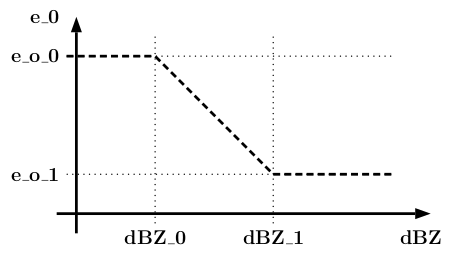
\includegraphics[width=\linewidth*\real{0.7}]{ramp_obserr_vr.png}\par
            The ramp can be definded by the following namelist parameters:
            \begin{tabitemize}
            \item[dBZ_0 =] \paramform{ramp_lowdbz_obserr_vr}
            \item[e_o_0 =] \paramform{maxval_obserr_vr}
            \item[dBZ_1 =] \paramform{ramp_highdbz_obserr_vr}
            \item[e_o_1 =] \paramform{baseval_obserr_vr} (if 1.0, then entire ramp to be interpreted as relative value)
            \end{tabitemize}
            Note that for reflectivity the observation error is always set to 1.0 and should be interpreted as a relative value.
          } & \spvierformat{\quetsche{0}} \\\hline
%
  & \quetsche{baseval_obserr_vr} & \quetsche{R (1)} &
          \spvierformat{\textbf{If \srcform{itype_obserr_vr$=$0}:} general constant value for radial wind observation error\par
            \textbf{If \srcform{itype_obserr_vr$=$1/2}:} obs error for dBZ-values $\ge$~\paramform{ramp_highdbz_obserr_vr} (e_o_1 in above sketch). \par
            IF baseval_obserr_vr=1.0, the observation error for radial wind is a relative error,
            which, in the data assimilation software, may be multiplied with observation errors which come from other sources (e.g. Desroziers-statistics).
         } & \spvierformat{\quetsche{1.0}}  \\\hline
%
  & \quetsche{maxval_obserr_vr} & \quetsche{R (1)} &
          \spvierformat{\textbf{If \srcform{itype_obserr_vr$=$1/2}:}
            obs error for dBZ-values $<$~\paramform{ramp_highdbz_obserr_vr} (e_o_1 in above sketch).
         } & \spvierformat{\quetsche{10.0}}  \\\hline
%
  & \quetsche{ramp_lowdbz_obserr_vr} & \quetsche{R (1)} &
          \spvierformat{\textbf{If \srcform{itype_obserr_vr$=$1/2}:}
            lower ramp dBZ-threshold (dBZ_0 in above sketch) for increasing observation error in radial wind.
         } & \spvierformat{\quetsche{0.0}}  \\\hline
%
  & \quetsche{ramp_highdbz_obserr_vr} & \quetsche{R (1)} &
          \spvierformat{\textbf{If \srcform{itype_obserr_vr$=$1/2}:}
            upper ramp dBZ-threshold (dBZ_1 in above sketch) for increasing observation error in radial wind.
         } & \spvierformat{\quetsche{10.0}}  \\\hline
%
  & \quetsche{itype_metric_refl_fdbk} & \quetsche{I (1)} & \spvierformat{Option for the specific metric of reflectivity $Z$ to write into feedback files (fof),
            for \paramform{lreadmeta_from_netcdf=.TRUE.} and \paramform{loutdbz=.TRUE.}:
            \begin{tabitemize}
            \item[1 =] write $\zeta$ in dBZ to feedback files ($\zeta=10\lg\frac{Z}{\text{1\,mm$^6$m$^{-3}$}}$)
            \item[2 =] convert to effective LWC = $0.004\,Z^{0.55}$ (g/m$^3$), but leave observation error unchanged from \paramform{itype_obserr_vr}
            \item[3 =] convert to effective LWC as for (2) and write a relative observation error for this LWC to fof,
              such that, when multpilied by a certain $\Delta dBZ$ (one-sided standard dev.) in the LETKF, this factor
              reproduces the weight which the equivalent dBZ-observation would have in the LETKF assuming a constant reflectivity error $\Delta dBZ$:\par
             $e_o = e_{o,lim} + 0.5\,a\,\frac{10^{0.1\,(\zeta+5dB)\,b} - 10^{0.1\,(\zeta-5dB)\,b}}{5dB}$\par
              with $a=0.004$, $b=0.55$. The additional constant $e_{o,lim}$ is added to prevent
              overly small observation errors for small LWC. It is the asymptotic value for LWC $\to$ 0.0 and can be given by namelist parameter \paramform{minval_obserr_lwc}.
            \end{tabitemize}
          } & \spvierformat{\quetsche{1}} \\\hline
%
  & \quetsche{minval_obserr_lwc} & \quetsche{R (1)} &
          \spvierformat{\textbf{If \srcform{itype_metric_refl_fdbk=3}:}
            asymptotic value for LWC $\to$ 0.0.
         } & \spvierformat{\quetsche{5E-4}}  \\\hline
%
% 
\multicolumn{2}{|l|}{\quetschee{labort_if_problems_obsfiles}} & \quetsche{L (1)} &
          \spvierformat{If .TRUE., abort the model run if serious problems with
            required observation files or metadata occur, i.e., no obs files at all,
            errors in file content, missing variables, missing or wrong station ID or scan strategy, etc.
            The default is to abort, but in operational runs this decision should be up to the user. \par
            If .FALSE., the model run continues but issues respective ERROR and WARNING messages.
          } & \spvierformat{\quetsche{.TRUE.} } \\\hline%%%
%
% 
\multicolumn{2}{|l|}{\quetschee{labort_if_problems_gribout}} & \quetsche{L (1)} &
          \spvierformat{If .TRUE., abort the model run if problems occur when writing grib output files (composites, volume scans) to disk by eccodes methods.
            In very few cases eccodes has issued an ``Input/Output error'' at runtime and the grib file could not be written correctly.
            The default is to abort in such a case, but in operational runs this decision should be up to the user. \par
            If .FALSE., the model run continues but issues respective ERROR and WARNING messages.
          } & \spvierformat{\quetsche{.TRUE.} } \\\hline%%%
%
%
\multicolumn{2}{|l|}{\quetschee{ldo_composite}} & \quetsche{L (1)} &
          \spvierformat{
            If .TRUE. generate one or more radar composite(s) of reflectivity from the simulated and (if available) observed volume scans for each time for which at least one of the radars has an observation timestep in the list \paramform{rs_meta($i$)\%obs_times}.\par
            A composite is generated by using one elevation of each station and, in areas of horizontal overlap,
            take the maximum of both (cf. Section~\ref{sec:intro:compo}). More than one composite using different elevations can be generated simultaneously.\par
            Composites are generated on a rotated lat-lon grid. In case of COSMO, it is
            equal to the model grid at the moment, but any other rotated lat-lon grid specifications would be possible
            in principle.\par 
            The reason to choose the model grid has been the fact that in the past
            only the COSMO-internal grib-output facilities have been used to write the composites to disk. However, in the
            meantime there is an own grib2-writer in EMVORADO, which is able to output any arbitrary lat-lon grids.\par
            The following namelist parameters in the derived type \paramform{comp_meta} define the composite grid independently
            from the model grid. Note that the default in case of COSMO is the COSMO-model grid itself.
          } & \spvierformat{\quetsche{.FALSE.} } \\\hline%%%
%
  & \quetsche{lcomposite_output} & \quetsche{\quetsche{L (1)}} &
          \spvierformat{Only effective if \srcform{ldo_composite=.TRUE.} or \srcform{ldo_bubbles=.TRUE.}: if \srcform{lcomposite_output=.TRUE.}
            EMVORADO uses it's own grib2-output facilities to write radar reflectivity composites to the
            output directory \srcform{ydirradarout} in its subdirectory \srcform{ysubdircomp}.\par
            See also Sections~\ref{sec:intro:compo} and~\ref{sec:comporemark} for more informations.\par
            Needs the local DWD grib sample file \srcform{DWD_rotated_ll_7km_G_grib2} from DWD's \srcform{grib_api} or \srcform{eccodes} distribution (center=EDZW).\par
            Otherwise, the composite output relies on the hosting model's output facilities. In the COSMO-model
            this is via the \srcform{/GRIBOUT/} namelist using parameter \srcform{yvarml='DBZCMPSIM','DBZCMPOBS'}, but this only
            works correctly if the composite grid is defined equal to the COSMO-model grid \textbf{and is not recommended any more}.\par
            \textbf{For ICON, \srcform{lcomposite_output=.TRUE.} is the only possibility to output the composites.}
          } & \spvierformat{\quetsche{.FALSE.} } \\\hline%%%
%
  & \quetsche{ysubdircomp} & \quetsche{C (\paramform{cmaxlen})} &
          \spvierformat{Subdirectory under \paramform{ydirradarout} for the storage of radar composites. If it starts with a ``/'', it is taken as an absolute path instead.
         } & \spvierformat{\quetsche{' '}}  \\\hline
%
  & \quetsche{composite_file_pattern} & \quetsche{C (\paramform{cmaxlen})} &
          \spvierformat{File pattern for composite output files. This enables a flexible definition of output file names as a mix of arbitrary text parts and the following placeholders:\par
            \begin{tabitemize}
              \item \paramform{<varname>} (optional): parameter identifier, default is \paramform{'dbzcmp'}
              \item \paramform{<simobs>} (optional): \paramform{'sim'} or \paramform{'obs'}, to be able to discriminate files with simulated and observed composites
              \item \paramform{<tmodelini>} (optional): absolute date and time of model start in format YYYYMMDDhhmmss
              \item \paramform{<tact>}: absolute model forecast date and time in format YYYYMMDDhhmmss
              \item \paramform{<tvvzact>}: relative forecast date and time in format DDhhmmss 
            \end{tabitemize}
            One of \paramform{<tact>} and \paramform{<tvvzact>} is mandatory, the respective other is then optional.
            \textbf{The default pattern is}\par \paramform{\textbf{'dbzcomp_<simobs>_<tmodelini>_<tact>.grb2'.}}
         } & \spvierformat{\quetsche{(see left)}}  \\\hline
%
%
  & \quetsche{comp_meta\%ni} & \quetsche{I (1)} & \spvierformat{Rotated lat/lon grid for the reflectivity composites: number of grid points in rotated meridional (``East-West'') direction.} &
          \spvierformat{\quetsche{COSMO = ie_tot}\par\quetsche{ICON = 651}}  \\\hline
%
  & \quetsche{comp_meta\%nj} & \quetsche{I (1)} & \spvierformat{Rotated lat/lon grid for the reflectivity composites: number of grid points in rotated zonal (``South-North'') direction.}
          & \spvierformat{\quetsche{COSMO = ie_tot}\par\quetsche{ICON = 716}}  \\\hline
%
  & \quetsche{comp_meta\%pollon} & \quetsche{R (1)} & \spvierformat{Rotated lat/lon grid for the reflectivity composites: geogr. longitude of rotated North-pole [\grad]. For a non-rotated grid set to -180.0.}
          & \spvierformat{\quetsche{COSMO = pollon}\par\quetsche{ICON = -170.0}} \\\hline
%
  & \quetsche{comp_meta\%pollat} & \quetsche{R (1)} & \spvierformat{Rotated lat/lon grid for the reflectivity composites: geogr. latitude of rotated North-pole [\grad]. For a non-rotated grid set to 90.0.}
          & \spvierformat{\quetsche{COSMO = pollat}\par\quetsche{ICON = 40.0}} \\\hline
%
  & \quetsche{comp_meta\%polgam} & \quetsche{R (1)} & \spvierformat{Rotated lat/lon grid for the reflectivity composites: angle between the North poles of two rotated grids [\grad]. Normally set to 0.0.}
          & \spvierformat{\quetsche{COSMO = polgam}\par\quetsche{ICON = 0.0}} \\\hline
%
  & \quetsche{comp_meta\%startlon} & \quetsche{R (1)} & \spvierformat{Rotated lat/lon grid for the reflectivity composites: lower left corner longitude in rotaded coordinates [\grad].}
          & \spvierformat{\quetsche{COSMO = startlon_tot}\par\quetsche{ICON = -7.5}} \\\hline
%
  & \quetsche{comp_meta\%startlat} & \quetsche{R (1)} & \spvierformat{Rotated lat/lon grid for the reflectivity composites: lower left corner latitude in rotaded coordinates [\grad].}
          & \spvierformat{\quetsche{COSMO = startlat_tot}\par\quetsche{ICON = -6.3}}  \\\hline
%
  & \quetsche{comp_meta\%dlon} & \quetsche{R (1)} & \spvierformat{Rotated lat/lon grid for the reflectivity composites: angular resolution [\grad] in rotated meridional direction.}
          & \spvierformat{\quetsche{COSMO = dlon}\par\quetsche{ICON = 0.02}} \\\hline
%
  & \quetsche{comp_meta\%dlat} & \quetsche{R (1)} & \spvierformat{Rotated lat/lon grid for the reflectivity composites: angular resolution [\grad] in rotated zonal direction.}
          & \spvierformat{\quetsche{COSMO = dlat}\par\quetsche{ICON = 0.02}} \\\hline
%
  & \quetsche{nel_composite} & \quetsche{I (1)} &
          \spvierformat{Number of composites to generate. The elevations for each station to apply for these composites
            are specified by the global background index list in the namelist parameter \srcform{eleindlist_for_composite_glob}.
            This list can be adjusted for each single station by \srcform{rs_meta($i$)\%eleindlist_for_composite_glob}.
            If the list is longer, the first \srcform{nel_composite} entries will be used. 
          } & \spvierformat{\quetsche{2}}  \\\hline
%
  & \quetsche{eleindlist_for_composite_glob} & \quetsche{I (nel_composite_max)} &
          \spvierformat{For \srcform{ldo_composite=.TRUE.}: global list of elevation indices to construct
            the composites. Will serve as the global default list for all stations, which can however be adjusted
            for each individual station by \srcform{rs_meta($i$)\%eleindlist_for_composite} (see Table~\ref{tab:dbzmeta}).
            The first element denotes the elevation index for the first composite, the second
            for the second composite, and so on.
            \begin{tabitemize}
            \item[1\dots \srcform{nel_max} =] Take this elevation of all volume scans. If a station has less elevations, it will be
              clipped to the largest elevation index of this station.
            \item[98 =] Take the precipitation scans (DWD-radar only).
              If precipitation scan is missing for certain stations, no data from these radars will appear in the composite.
            \item[99 =] Take the vertical maximum of all elevations of all radars
            \item[other: ] Not allowed, model run will be terminated.
            \end{tabitemize}
            For precipitation scans: the elevations for lat/lon computations will not be the true elevations
            but the nominal elevation (either 0.4\grad, 0.59\grad, 0.8\grad, or 1.3\grad).}
          & \spvierformat{\quetsche{(/ 1, 2 /)}}  \\\hline
%
  & \quetsche{levelidlist_for_composite_glob} & \quetsche{I (nel_composite_max)} &
          \spvierformat{For \srcform{ldo_composite=.TRUE.}: global list of grib2 level identifiers
            for the composites. The first identifier in the list corresponds to the first composite
            in the list \srcform{eleindlist_for_composite_glob}, the second identifier to the second composite and so on.\\
            This identifier is written to the grib2-keys \srcform{level} and \srcform{scaledValueOfFirstFixedSurface}.
            Negative values lead to a crash of \srcform{grib_api} and are not allowed.}
          & \spvierformat{\quetsche{eleindlist_for_composite_glob}}  \\\hline
%
  & \quetsche{lsmooth_composite_bub_glob} & \quetsche{L (1)} & \spvierformat{Not yet in the namelist, up to now hardcoded in \srcform{radar_namelist_read.f90}} & \spvierformat{\quetsche{.FALSE.}}  \\\hline
%
  & \quetsche{nsmoothpoints_for_comp_bub_glob} & \quetsche{I (1)} & \spvierformat{Not yet in the namelist, up to now hardcoded in \srcform{radar_namelist_read.f90}} & \spvierformat{\quetsche{9}}  \\\hline
%
  & \quetsche{nfilt_for_comp_bub_glob} & \quetsche{I (1)} & \spvierformat{Not yet in the namelist, up to now hardcoded in \srcform{radar_namelist_read.f90}} & \spvierformat{\quetsche{1}}  \\\hline
%
%
\multicolumn{2}{|l|}{\quetschee{ldo_bubbles}} & \quetsche{L (1)} &
          \spvierformat{Enable the ``warm bubble generator'' to trigger missing convective cells in the model by artificial warm bubbles
            inspired by \citeP{weisman1982}. The detection of missing convective cells is based on simulated and observed radar composites  (cf. Section~\ref{sec:intro:compo}).
            The bubble's type, amplitude, size, shape and duration can be defined by additional namelist parameters below.
            The exact locations and model times are detected by the bubble generator.\par
            More informations can be found in Section~\ref{sec:warmbub}.\par
            Uses the same composite grid (\srcform{comp_meta\%\dots}) and elevation index conventions as for \srcform{ldo_composite=.TRUE.}.\par
            Only effective if \srcform{lreadmeta_from_netcdf=.TRUE.}}
          & \spvierformat{\quetsche{.FALSE.} } \\\hline%%%
%
  & \quetsche{eleind_for_composite_bub_glob} & \quetsche{I (1)} &
          \spvierformat{
              For \srcform{ldo_bubbles=.TRUE.}: elevation index to be used for the composite to detect the need for warm bubbles.
              Same valid values as for \srcform{eleindlist_for_composite_glob}.
            }
            & \spvierformat{\quetsche{-99}}  \\\hline
%
  & \quetsche{lcomposite_output_bub} & \quetsche{\quetsche{L (1)}} &
          \spvierformat{Only effective if \srcform{ldo_bubbles=.TRUE.}: if \srcform{lcomposite_output_bub=.TRUE.}
            EMVORADO uses it's own grib2-output facilities to write radar reflectivity composites to the
            output directory \srcform{ydirradarout} in its subdirectory \srcform{ysubdircomp}.\par
            See also Sections~\ref{sec:intro:compo} and~\ref{sec:comporemark} for more informations.\par
            Needs the local DWD grib sample file \srcform{DWD_rotated_ll_7km_G_grib2} from DWD's \srcform{grib_api} or \srcform{eccodes} distribution (center=EDZW).\par
            Otherwise, the composite output relies on the hosting model's output facilities. In the COSMO-model
            this is via the \srcform{/GRIBOUT/} namelist using parameter \srcform{yvarml='DBZCMPSIM','DBZCMPOBS'}, but this only
            works correctly if the composite grid is defined equal to the COSMO-model grid \textbf{and is not recommended any more}.\par
            \textbf{For ICON, \srcform{lcomposite_output_bub=.TRUE.} is the only possibility to output the composites.}
          } & \spvierformat{\quetsche{.FALSE.} } \\\hline%%%
%
  & \quetsche{composite_file_pattern_bub} & \quetsche{C (\paramform{cmaxlen})} &
          \spvierformat{File pattern for bubble generator composite output files. This enables a flexible definition of output file names as a mix of arbitrary text parts and the following placeholders:\par
            \begin{tabitemize}
              \item \paramform{<varname>} (optional): parameter identifier, default is \paramform{'dbzcmpbub'}
              \item \paramform{<simobs>} (optional): \paramform{'sim'} or \paramform{'obs'}, to be able to discriminate files with simulated and observed composites
              \item \paramform{<tmodelini>} (optional): absolute date and time of model start in format YYYYMMDDhhmmss
              \item \paramform{<tact>}: absolute model forecast date and time in format YYYYMMDDhhmmss
              \item \paramform{<tvvzact>}: relative forecast date and time in format DDhhmmss 
            \end{tabitemize}
            One of \paramform{<tact>} and \paramform{<tvvzact>} is mandatory, the respective other is then optional.
            \textbf{The default pattern is}\par \paramform{\textbf{'dbzcompbub_<simobs>_<tmodelini>_<tact>.grb2'.}}
         } & \spvierformat{\quetsche{(see left)}}  \\\hline
%
  & \quetsche{comp_meta_bub\%ni} & \quetsche{I (1)} & \spvierformat{Rotated lat/lon grid for the reflectivity composites: number of grid points in rotated meridional (``East-West'') direction.} &
          \spvierformat{\quetsche{COSMO = ie_tot}\par\quetsche{ICON = 651}}  \\\hline
%
  & \quetsche{comp_meta_bub\%nj} & \quetsche{I (1)} & \spvierformat{Rotated lat/lon grid for the reflectivity composites: number of grid points in rotated zonal (``South-North'') direction.}
          & \spvierformat{\quetsche{COSMO = ie_tot}\par\quetsche{ICON = 716}}  \\\hline
%
  & \quetsche{comp_meta_bub\%pollon} & \quetsche{R (1)} & \spvierformat{Rotated lat/lon grid for the reflectivity composites: geogr. longitude of rotated North-pole [\grad]. For a non-rotated grid set to -180.0.}
          & \spvierformat{\quetsche{COSMO = pollon}\par\quetsche{ICON = -170.0}} \\\hline
%
  & \quetsche{comp_meta_bub\%pollat} & \quetsche{R (1)} & \spvierformat{Rotated lat/lon grid for the reflectivity composites: geogr. latitude of rotated North-pole [\grad]. For a non-rotated grid set to 90.0.}
          & \spvierformat{\quetsche{COSMO = pollat}\par\quetsche{ICON = 40.0}} \\\hline
%
  & \quetsche{comp_meta_bub\%polgam} & \quetsche{R (1)} & \spvierformat{Rotated lat/lon grid for the reflectivity composites: angle between the North poles of two rotated grids [\grad]. Normally set to 0.0.}
          & \spvierformat{\quetsche{COSMO = polgam}\par\quetsche{ICON = 0.0}} \\\hline
%
  & \quetsche{comp_meta_bub\%startlon} & \quetsche{R (1)} & \spvierformat{Rotated lat/lon grid for the reflectivity composites: lower left corner longitude in rotaded coordinates [\grad].}
          & \spvierformat{\quetsche{COSMO = startlon_tot}\par\quetsche{ICON = -7.5}} \\\hline
%
  & \quetsche{comp_meta_bub\%startlat} & \quetsche{R (1)} & \spvierformat{Rotated lat/lon grid for the reflectivity composites: lower left corner latitude in rotaded coordinates [\grad].}
          & \spvierformat{\quetsche{COSMO = startlat_tot}\par\quetsche{ICON = -6.3}}  \\\hline
%
  & \quetsche{comp_meta_bub\%dlon} & \quetsche{R (1)} & \spvierformat{Rotated lat/lon grid for the reflectivity composites: angular resolution [\grad] in rotated meridional direction.}
          & \spvierformat{\quetsche{COSMO = dlon}\par\quetsche{ICON = 0.02}} \\\hline
%
  & \quetsche{comp_meta_bub\%dlat} & \quetsche{R (1)} & \spvierformat{Rotated lat/lon grid for the reflectivity composites: angular resolution [\grad] in rotated zonal direction.}
          & \spvierformat{\quetsche{COSMO = dlat}\par\quetsche{ICON = 0.02}} \\\hline
%
  & \quetsche{lsmooth_composite_bub_glob} & \quetsche{L (1)} & \spvierformat{For \srcform{ldo_bubbles=.TRUE.}: If composite is to be smoothed by binomial filter. Not yet in the namelist, up to now hardcoded in \srcform{radar_namelist_read.f90}} & \spvierformat{\quetsche{.FALSE.}}  \\\hline
%
  & \quetsche{nsmoothpoints_for_comp_bub_glob} & \quetsche{I (1)} & \spvierformat{For \srcform{ldo_bubbles=.TRUE.}: width of symetric 2D binomial smoother in grid points. Not yet in the namelist, up to now hardcoded in \srcform{radar_namelist_read.f90}} & \spvierformat{\quetsche{9}}  \\\hline
%
  & \quetsche{nfilt_for_comp_bub_glob} & \quetsche{I (1)} & \spvierformat{For \srcform{ldo_bubbles=.TRUE.}: number of consecutive applications of the smoother. Not yet in the namelist, up to now hardcoded in \srcform{radar_namelist_read.f90}} & \spvierformat{\quetsche{1}}  \\\hline
%
  & \quetsche{tstart_bubble_search} & \quetsche{R (1)} & \spvierformat{For \srcform{ldo_bubbles=.TRUE.}: start time for the bubble generator [s since model start].} & \spvierformat{\quetsche{0.0}}  \\\hline
%
  & \quetsche{dt_bubble_search} & \quetsche{R (1)} & \spvierformat{For \srcform{ldo_bubbles=.TRUE.}: time interval from one automatic bubble search to the next [s].} & \spvierformat{\quetsche{900.0}}  \\\hline
%
  & \quetsche{tend_bubble_search} & \quetsche{R (1)} & \spvierformat{For \srcform{ldo_bubbles=.TRUE.}: end time for the bubble generator [s since model start].} & \spvierformat{\quetsche{HUGE(1.0_dp)}}  \\\hline
%
  & \quetsche{t_offset_bubble_trigger_async} & \quetsche{R (1)} & \spvierformat{For \srcform{ldo_bubbles=.TRUE.} and in case of asynchronous radar IO for runtime optimization: time delay of (advection corrected) bubble triggering after detection step [s]. In an ideal world, one would set this delay to 0, but this prevents the worker PEs to continue with model integration in parallel to the IO PEs, which detect, among other tasks, the missing cells. If triggering is delayed, the worker PEs can continue for this amout of time until they gather the bubble parameters from the IO PEs and trigger the warm bubbles.} & \spvierformat{\quetsche{0.0}}  \\\hline
%
  & \quetsche{prob_bubble} & \quetsche{R (1)} & \spvierformat{For \srcform{ldo_bubbles=.TRUE.}: probability of triggering a bubble when it is found [0-1].} & \spvierformat{\quetsche{1.0}}  \\\hline
%
  & \quetsche{lbub_isolated} & \quetsche{L (1)} & \spvierformat{For \srcform{ldo_bubbles=.TRUE.}: check that the bubbles are isolated from other objects in observations.} & \spvierformat{\quetsche{.FALSE.}}  \\\hline
%
  & \quetsche{maxdim_obs} & \quetsche{R (1)} & \spvierformat{For \srcform{ldo_bubbles=.TRUE.}: maximum dimension of missing cell that can trigger a bubble (larger objects are not targeted) [m].} & \spvierformat{\quetsche{75000.0}}  \\\hline
%
  & \quetsche{threshold_obs} & \quetsche{R (2)} & \spvierformat{For \srcform{ldo_bubbles=.TRUE.}: thresholds for observed composite that define the minimum dBZ in an object- and the high intensity region [dBZ].} & \spvierformat{\quetsche{(/25.0, 30.0/)}}  \\\hline
%
  & \quetsche{threshold_mod} & \quetsche{R (2)} & \spvierformat{For \srcform{ldo_bubbles=.TRUE.}: thresholds for simulated composite that define the minimum dBZ in an object- and the high intensity region [dBZ].} & \spvierformat{\quetsche{(/25.0, 30.0/)}}  \\\hline
%
  & \quetsche{areamin_obs} & \quetsche{R (2)} & \spvierformat{For \srcform{ldo_bubbles=.TRUE.}: minimum area in observed composite of the object- and high intensity region for detecting an object  [m$^2$]} & \spvierformat{\quetsche{(/ 25e6, 9e6/)}}  \\\hline
%
  & \quetsche{areamin_mod} & \quetsche{R (2)} & \spvierformat{For \srcform{ldo_bubbles=.TRUE.}: minimum area in simulated composite of the object- and high intensity region for detecting an object  [m$^2$]} & \spvierformat{\quetsche{(/ 25e6, 9e6/)}}  \\\hline
%
  & \quetsche{mult_dist_obs} & \quetsche{R (1)} & \spvierformat{For \srcform{ldo_bubbles=.TRUE.}: multiplicative axis lenght factor for the observed object to define the minimal required ellisoidal distance frame required for simulated objects to be defined as ``isolated'' and trigger bubbles [-].} & \spvierformat{\quetsche{1.0}}  \\\hline
%
  & \quetsche{mult_dist_mod} & \quetsche{R (1)} & \spvierformat{For \srcform{ldo_bubbles=.TRUE.}: multiplicative axis lenght factor for simulated objects to define the minimal required ellisoidal distance frame required forthe simulated objects to be defined as ``isolated'' and trigger bubbles [-].} & \spvierformat{\quetsche{1.0}}  \\\hline
%
  & \quetsche{add_dist_obs} & \quetsche{R (1)} & \spvierformat{For \srcform{ldo_bubbles=.TRUE.}: additive axis increase for the observed object to define the minimal required ellisoidal distance frame required for simulated objects to be defined as ``isolated'' and trigger bubbles [m]. Is applied after mult_dist_obs.} & \spvierformat{\quetsche{1.0}}  \\\hline
%
  & \quetsche{add_dist_mod} & \quetsche{R (1)} & \spvierformat{For \srcform{ldo_bubbles=.TRUE.}: additive axis increase for simulated objects to define the minimal required ellisoidal distance frame required forthe simulated objects to be defined as ``isolated'' and trigger bubbles [-]. Is applied after mult_dist_mod.} & \spvierformat{\quetsche{1.0}}  \\\hline
%
  & \quetsche{dt_bubble_advect} & \quetsche{R (1)} & \spvierformat{For \srcform{ldo_bubbles=.TRUE.}: time scale for downstream advection of automatic bubbles [sec].} & \spvierformat{\quetsche{300.0}}  \\\hline
%
  & \quetsche{zlow_meanwind_bubble_advect} & \quetsche{I (1)} & \spvierformat{For \srcform{ldo_bubbles=.TRUE.}: the lower bound of averaging height interval for computing the integral-averaged advection speed for automatic bubbles [m MSL].} & \spvierformat{\quetsche{3000.0}}  \\\hline
%
  & \quetsche{zup_meanwind_bubble_advect} & \quetsche{I (1)} & \spvierformat{For \srcform{ldo_bubbles=.TRUE.}: the lower bound of averaging height interval for computing the integral-averaged advection speed for automatic bubbles [m MSL].} & \spvierformat{\quetsche{6000.0}}  \\\hline
%
  & \quetsche{bubble_type} & \quetsche{C (12)} & \spvierformat{For \srcform{ldo_bubbles=.TRUE.}: type of the bubble (\srcform{'cos-hrd'} or \srcform{'cos-instant'})} & \spvierformat{\quetsche{\srcform{'cos-hrd'}}}  \\\hline
%
  & \quetsche{bubble_heatingrate} & \quetsche{R (1)} & \spvierformat{For \srcform{ldo_bubbles=.TRUE.}: heating rate for the bubbles of type 'cos-hrd' [K/s]} & \spvierformat{\quetsche{0.015}}  \\\hline
%
  & \quetsche{bubble_timespan} & \quetsche{R (1)} & \spvierformat{For \srcform{ldo_bubbles=.TRUE.}: timespan for heating the bubbles of type 'cos-hrd' [s] } & \spvierformat{\quetsche{200.0}}  \\\hline
%
  & \quetsche{bubble_dT} & \quetsche{R (1)} & \spvierformat{For \srcform{ldo_bubbles=.TRUE.}: temperature disturbance for the bubbles of type 'cos-instant' [K] } & \spvierformat{\quetsche{3.0}}  \\\hline
%
  & \quetsche{bubble_centz} & \quetsche{R (1)} & \spvierformat{For \srcform{ldo_bubbles=.TRUE.}: center height MSL (Z) of the bubbles [m]} & \spvierformat{\quetsche{2000.0}}  \\\hline
%
  & \quetsche{bubble_radx} & \quetsche{R (1)} & \spvierformat{For \srcform{ldo_bubbles=.TRUE.}: horizontal radius (main axis) in X-dir of the bubbles [m]} & \spvierformat{\quetsche{7500.0}}  \\\hline
%
  & \quetsche{bubble_rady} & \quetsche{R (1)} & \spvierformat{For \srcform{ldo_bubbles=.TRUE.}: horizontal radius (main axis) in Y-dir of the bubbles [m]} & \spvierformat{\quetsche{7500.0}}  \\\hline
%
  & \quetsche{bubble_radz} & \quetsche{R (1)} & \spvierformat{For \srcform{ldo_bubbles=.TRUE.}: vertical radius in Z-dir of the bubbles [m]} & \spvierformat{\quetsche{1400.0}}  \\\hline
%
  & \quetsche{bubble_rotangle} & \quetsche{R (1)} & \spvierformat{For \srcform{ldo_bubbles=.TRUE.}: rotation angle of the main axes of bubbles [\grad]} & \spvierformat{\quetsche{0.0}}  \\\hline
%
  & \quetsche{bubble_holdrhconst} & \quetsche{L (1)} & \spvierformat{For \srcform{ldo_bubbles=.TRUE.}: switch to choose if RH should kept constant during heating or not} & \spvierformat{\quetsche{.TRUE.}}  \\\hline
%
  & \quetsche{bubble_addnoise} & \quetsche{L (1)} & \spvierformat{For \srcform{ldo_bubbles=.TRUE.}: switch to activate some random noise on the bubbles with a relative amplitude of \paramform{bubble_dT_noise}} & \spvierformat{\quetsche{.FALSE.}}  \\\hline
%
  & \quetsche{bubble_dT_noise} & \quetsche{R (1)} & \spvierformat{For \srcform{ldo_bubbles=.TRUE.} and in case of \paramform{bubble_addnoise_T=.true.}, \paramform{bubble_dT_noise} is the relative noise level $\eta$, such that $\Delta T_{bubble}=\Delta T_{bubble,0} (1+\eta)$ with $\eta\in [-1,1]$)} & \spvierformat{\quetsche{0.1}}  \\\hline
%
%
\multicolumn{2}{|l|}{\quetschee{ldo_bubbles_manual}} & \quetsche{L (1)} &
          \spvierformat{Setting this switch to true enables to manually specify artificial convection triggers in
            real case simulations. This nees an explicit namelist \srcform{/ARTIFCTL/} in a file \srcform{INPUT_IDEAL} as
            described in \citeP{blahak2015b} with the relevant convection trigger parameters for atmospheric
            temperature- and humidity disturbances. Disturbances in the soil and all other namelist parameters
            of \srcform{/ARTIFCTL/} will be ignored.
          } & \spvierformat{\quetsche{.FALSE.} } \\\hline%%%
% 
%
\multicolumn{2}{|l|}{\quetschee{lwrite_ready}} & \quetsche{L (1)} &
          \spvierformat{Switch to enable the writing of so-called READY-files, cf. Section~\ref{sec:output:ready}.
            If .TRUE., files having names like \paramform{READY_EMVORADO_20200215123500} per default are written into the
            output directory for READY-files at the end of each EMVORADO output time step. Postprocessing jobs on output files for
            this timestep may start as soon as the READY-file exists, concurrently to the model run.\par
            The name of the ready file can be configured by \paramform{ready_file_pattern}, see below.
          } & \spvierformat{\quetsche{.FALSE.} } \\\hline

%
  & \quetsche{ydir_ready_write} & \quetsche{C (\paramform{cmaxlen})} &
          \spvierformat{For \paramform{lwrite_ready=.TRUE.}:\par
            absolute path for writing READY-files to disk. If empty, READY-files are written to \paramform{ydirradarout}.
          }
          & \spvierformat{\quetsche{' '}}  \\\hline
%
  & \quetsche{ready_file_pattern} & \quetsche{C (\paramform{cmaxlen})} &
          \spvierformat{For \paramform{lwrite_ready=.TRUE.}:\par
            File pattern for READY-files. This enables a flexible definition of READY filenames as a mix of arbitrary text parts and the following placeholders:\par
            \begin{tabitemize}
              \item \paramform{<tmodelini>} (optional): absolute date and time of model start in format YYYYMMDDhhmmss
              \item \paramform{<tact>}: absolute model forecast date and time in format YYYYMMDDhhmmss
              \item \paramform{<tvvzact>}: relative forecast date and time in format DDhhmmss 
            \end{tabitemize}
            One of \paramform{<tact>} and \paramform{<tvvzact>} is mandatory, the respective other is then optional.
            \textbf{The default pattern is}\par \paramform{\textbf{'READY_EMVORADO_<tact>'.}}
         } & \spvierformat{\quetsche{(see left)}}  \\\hline
%TRIM(path)//'READY_EMVORADO_'//TRIM(model_validtime)
%
%ready_file_pattern
%
% & \quetsche{GAGA} & \quetsche{I (1)} & \spvierformat{fafa \begin{tabitemize}
%          \item idbg_artif_level $>$ 0
%          \item idbg_artif_level $>$ 3 : additionally, write ASCII-files
%          \end{tabitemize}} &  \spvierformat{\quetsche{idbg_artif_level_d = 0} }  \\\hline
%
%%%%%
%%%%%% TEMPLATE FOR A PRIMARY NAMELIST PARAMETER (NOT DEPENDENT ON ANY OTHER):
% \multicolumn{2}{|l|}{\quetschee{}} & \quetsche{L (1)} &
%           \spvierformat{} & \spvierformat{\quetsche{} } \\\hline%%%
%%%%%
%%%%% TEMPLATE FOR A SECONDARY (DEPENDENT) NAMELIST PARAMETER:
% & \quetsche{} & \quetsche{I (1)} & \spvierformat{} & \spvierformat{\quetsche{}}  \\\hline
%%%%%
\end{longtable}
\end{small}


\newpage

\subsubsection{Station metadata in namelist \srcform{rs_meta($i$)} type in \srcform{/RADARSIM_PARAMS/}}
\label{sec:nml:rsmeta}


\begin{small}

%%% Column widths of the following 5-column table:
\setlength{\lenspeins}{0.02cm}   % This is the indentation of basic parameters as opposed to dependend parameters
\setlength{\lenspzwei}{2.4cm}
\setlength{\lenspdrei}{2.0cm}
\setlength{\lenspvier}{8.0cm}
\setlength{\lenspfunf}{2.4cm}

\setlength{\extrarowheight}{0.25\baselineskip}
\begin{longtable}{|p{\lenspeins}p{\lenspzwei}|>{\hspace*{\extrarowheight}}p{\lenspdrei}|p{\lenspvier}<{\vspace*{\extrarowheight}}|p{\lenspfunf}|}
\caption{\label{tab:rsmeta}Table of radar station metadata for station $i$ in \srcform{/RADARSIM_PARAMS/} in an element \srcform{rs_meta($i$)} of the vector \srcform{rs_meta} of derived type \srcform{radar_meta_type} (module \srcform{radar_data.f90}). 
Kind abbreviations: ``I''~= INTEGER, ``R''~= REAL/DOUBLE, ``C''~=CHARACTER, ``L''~= LOGICAL, ``T''~= Derived TYPE. The defaults depend on \srcform{rs_meta($i$)\%icountry} respectively namelist parameter \srcform{icountry}. In this table, we assume \srcform{rs_meta($i$)\%icountry}~= 1 (Germany).}\\
\hline
\multicolumn{2}{|l|}{\quetschee{\normalsize{\textbf{Name rs_meta($i$)\%}}}} & \quetsche{\normalsize{\textbf{Kind (Dim.)}}} & 
                     \normalsize{\textbf{Description / Remarks}} & \normalsize{\textbf{Default}} \\
\hline
\endfirsthead
\caption{continued}\\
\hline
\multicolumn{2}{|l|}{\quetschee{\normalsize{\textbf{Name rs_meta($i$)\%}}}} & \quetsche{\normalsize{\textbf{Kind (Dim.)}}} & 
                     \normalsize{\textbf{Description / Remarks}} & \normalsize{\textbf{Default}} \\
\hline
\endhead
%%%
\multicolumn{2}{|l|}{\quetschee{\%icountry}} & \quetsche{I (1)} &
          \spvierformat{Country flag for this radar. Is initialized by the global namelist parameter \srcform{icountry}
            and can be altered for each individual station $i$ via namelist.
            Current possible values are:
            \begin{tabitemize}
            \item[1 =] Germany (DWD)
            \item[2 =] Switzerland (MeteoSwiss)
            \item[3 =] Italy (ARPA-SIMC)            
            \end{tabitemize}
            This choice influences the defaults for the below type components in \srcform{rs_meta($i$). In this table,
            we have assumed \srcform{rs_meta($i$)\%icountry}~= 1}
          } & \spvierformat{\quetsche{\srcform{icountry}} } \\\hline%%%
%
%
\multicolumn{2}{|l|}{\quetschee{\%station_id}} & \quetsche{I (1)} &
          \spvierformat{WMO station ID of the radar station (country code + national ID). This ID should be explicitly given in the namelist for each station block $i$.} & \spvierformat{\quetsche{999999} } \\\hline%%%
%
%
\multicolumn{2}{|l|}{\quetschee{\%station_name}} & \quetsche{C (3)} &
          \spvierformat{3-character station akronym.} & \spvierformat{\quetsche{'XXX'} } \\\hline%%%
%
%
\multicolumn{2}{|l|}{\quetschee{\%lambda}} & \quetsche{R (1)} &
          \spvierformat{Radar wavelength [m]. For efficiency reasons, it can be advantageous not to choose the very exact wavelength.
            For example, in a network of C-Band radars, choose all wavelengths to be the same 0.055\,m to enable re-use of simulated 
            grid-point reflectivity values from one radar station to the next to save computing time.} & \spvierformat{\quetsche{0.055} } \\\hline%%%
%
%
\multicolumn{2}{|l|}{\quetschee{\%lon}} & \quetsche{R (1)} &
          \spvierformat{Station geographical longitude [deg]} & \spvierformat{Domain center} \\\hline%%%
%
%
\multicolumn{2}{|l|}{\quetschee{\%lat}} & \quetsche{R (1)} &
          \spvierformat{Station geographical latitude [deg]} & \spvierformat{Domain center} \\\hline%%%
%
%
\multicolumn{2}{|l|}{\quetschee{\%alt_agl_mod}} & \quetsche{R (1)} &
          \spvierformat{Station height above model orography [m]. Represents the height of the radar antenna above ground.} & \spvierformat{\quetsche{50.0} } \\\hline%%%
%
%
\multicolumn{2}{|l|}{\quetschee{\%alt_msl}} & \quetsche{R (1)} &
          \spvierformat{Station height above MSL [m]. This height will internally used for all height-related computations.
          If it is set to the value -9999.99, it will automatically be computed as
        \srcform{rs_meta($i$)\%alt_agl_mod} plus model orography height at the station location.} & \spvierformat{\quetsche{-9999.99} } \\\hline%%%
%
%
\multicolumn{2}{|l|}{\quetschee{\%alt_msl_true}} & \quetsche{R (1)} &
          \spvierformat{True station height MSL [m] as read from observation files [m].\par Only relevant if \srcform{lreadmeta_from_netcdf=.TRUE.}} & \spvierformat{\quetsche{-9999.99} } \\\hline%%%
%
%
\multicolumn{2}{|l|}{\quetschee{\%naz}} & \quetsche{I (1)} &
          \spvierformat{Number of nominal azimuths (radials) within a PPI-elevation} & \spvierformat{\quetsche{360} } \\\hline%%%
%
%
\multicolumn{2}{|l|}{\quetschee{\%az_start}} & \quetsche{R (1)} &
          \spvierformat{Start azimuth of first radial relative to True North [deg]} & \spvierformat{\quetsche{0.0} } \\\hline%%%
%
%
\multicolumn{2}{|l|}{\quetschee{\%az_inc}} & \quetsche{R (1)} &
          \spvierformat{Azimuth increment [deg] from radial to radial} & \spvierformat{\quetsche{1.0} } \\\hline%%%
%
%
\multicolumn{2}{|l|}{\quetschee{\%nra}} & \quetsche{I (1)} &
          \spvierformat{Max. number of range bins occuring in a volume scan (sometimes, higher elevations have less range bins, but here the maximum number of all elevations is required)} & \spvierformat{\quetsche{124} } \\\hline%%%
%
%
\multicolumn{2}{|l|}{\quetschee{\%ra_inc}} & \quetsche{R (1)} &
          \spvierformat{Range increment [m] from bin to bin anlong a radial} & \spvierformat{\quetsche{1000.0} } \\\hline%%%
%
%
\multicolumn{2}{|l|}{\quetschee{\%nel}} & \quetsche{I (1)} &
          \spvierformat{Number of elevations of the PPI volume scan} & \spvierformat{\quetsche{18} } \\\hline%%%
%
%
\multicolumn{2}{|l|}{\quetschee{\%el_arr}} & \quetsche{R (nel_max)} &
          \spvierformat{List of nominal elevation angles [deg] of the PPI volume scan. The list should contain \srcform{rs_meta($i$)\%nel} elements.\par 
            These elevation angles are actually used for all computations and, in case of \srcform{lreadmeta_from_netcdf=.TRUE.},
            preferred over the ``true'' elevation angles given in some observation files. One exception are DWD's ``precipitation scans'' with their horizon-following nominal elevations.
            Here, just one ``fake'' elevation out of (0.4, 0.59, 0.8, 1.3) has to be given and \srcform{rs_meta($i$)\%nel} = 1. However, this only works for
            stations with a valid German station id, and the elevation as function of azimuth depends on \srcform{rs_meta($i$)\%station_id} as defined in
            the module \srcform{radar_elevations_precipscan.incf}.
          }
     & \spvierformat{(/0.5, 1.5, 2.5, 3.5, 4.5, 5.5, 6.5, 7.5, 8.5,
                       9.5, 11.0, 13.0, 15.0, 17.0, 19.0, 23.0, 29.0, 37.0/) } \\\hline%%%
%
%
\multicolumn{2}{|l|}{\quetschee{\%scanname}} & \quetsche{C (10)} &
        \spvierformat{This parameter cannot really be set by namelist but is automatically determined from \srcform{rs_meta($i$)\%el_arr}.
            It appears in the namelist control output file \srcform{YUSPECIF_RADAR} (COSMO) respectively \srcform{nml.emvorado.log} (ICON) and
            is part of some of EMVORADO's output file names. It consists of 'PRECIP' (if DWD precipitation scan) or
            'PPI' plus a 4-digit number representing the average elevation angle of the scan times 10. Examples are 'PPI0080', 'PRECIP'.} & \spvierformat{\quetsche{'PPI0119'} } \\\hline%%%
%
%
\multicolumn{2}{|l|}{\quetschee{\%nel_default}} & \quetsche{I (nscanstrategies_max)} &
          \spvierformat{Only relevant if \srcform{lreadmeta_from_netcdf=.TRUE.}: in this case, each radar observation file has to conform to one of certain
            allowed scan strategies. If not, the corresponding station is discarded from the simulation. \srcform{nel_default} is the number of elevations for each of these allowed default scan strategies.
          Depends on \srcform{rs_meta($i$)\%icountry} and is predefined accordingly in the module \srcform{radar_obs_meta_list.f90}, so no need to specify it explicitly in the namelist.} & \spvierformat{(/18, 18, 10, 10, 1, 1, 1, 1, 3, 3/) } \\\hline%%%
%
%
\multicolumn{2}{|l|}{\quetschee{\%el_arr_default}} & \spvierformat{R (nel_max, \quetsche{nscanstrategies_max)}} &
          \spvierformat{Only relevant if \srcform{lreadmeta_from_netcdf=.TRUE.}: array of the \srcform{rs_meta($i$)\%nel_default} allowed default scan strategies. Again depends on \srcform{rs_meta($i$)\%icountry} and is predefined accordingly in the module \srcform{radar_obs_meta_list.f90}, so no need to specify it explicitly in the namelist.} & \spvierformat{See function \quetsche{\srcform{get_meta_proto_dwd()}} in \srcform{radar_obs_meta_list.f90} } \\\hline%%%
%
%
\multicolumn{2}{|l|}{\quetschee{\%el_arr_obs}} & \quetsche{R (nel_max)} &
          \spvierformat{Only relevant if \srcform{lreadmeta_from_netcdf=.TRUE.}:
            List of ``true'' elevations [deg] from observation files, used for cross-checking with \srcform{rs_meta($i$)\%el_arr}. Will be filled automatically during reading of observation files.}
      & \spvierformat{(/0.5, 1.5, 2.5, 3.5, 4.5, 5.5, 6.5, 7.5, 8.5,
                       9.5, 11.0, 13.0, 15.0, 17.0, 19.0, 23.0, 29.0, 37.0/) } \\\hline%%%
%
%
\multicolumn{2}{|l|}{\quetschee{\%obs_times}} & \quetsche{R (nobstimes_max)} &
          \spvierformat{List of observation times in seconds since model run start. Any values $\ge 0.0$ define the desired times for simulating volume scans of this radar station.
            If no value $\ge 0.0$ is given, observation times are automatically computed from the parameters \srcform{rs_meta($i$)\%nobs_times} and \srcform{rs_meta($i$)\%dt_obs}.}
          & \spvierformat{\quetsche{-999.9} } \\\hline%%%
%
%
\multicolumn{2}{|l|}{\quetschee{\%dt_obs}} & \quetsche{R (3)} &
          \spvierformat{Time triplet \paramform{from-time,to-time,increment} for building the list
              of regularily spaced observation times [s since nominal model start time].\par
              Only relevant if no \srcform{rs_meta($i$)\%obs_times} $\ge 0.0$ are given.\par
              The list of \srcform{rs_meta($i$)\%obs_times} is computed in intervals of dt_obs starting
              from \paramform{from-time} until \srcform{rs_meta($i$)\%nobs_times} steps, or, if \srcform{nobs_times}
              is not set, until \paramform{to-time}. If \paramform{from-time} is given as a missing value,
              the series of obs times starts approximately at the nominal model start time ---
              which might be negative for IAU runs --- and is synchonized to time 0.0\,s.\par
              For backwards compatibility, one can also give only one value in the namelist, which is interpreted as the increment
              and automatically shifted to the correct position in the triplet. \paramform{from-time} and \paramform{to-time} are set to -999.9 in this case.\par
              Note: the default is given in this old notation, only one value!
            } & \spvierformat{\quetsche{300.0}} \\\hline%%%
%
%
\multicolumn{2}{|l|}{\quetschee{\%nobs_times}} & \quetsche{I (1)} &
          \spvierformat{Number of observation times.\par
            Only relevant if no \srcform{rs_meta($i$)\%obs_times} $\ge 0.0$ are given.\par
            If $<0$, the list of \srcform{rs_meta($i$)\%obs_times} is computed to fill the entire model simulation time with
            observation times in regular intervals of \srcform{rs_meta($i$)\%dt_obs}.} & \spvierformat{\quetsche{-999} } \\\hline%%%
%
%
\multicolumn{2}{|l|}{\quetschee{\%lobstimes_ovwrt_recalc}} & \quetsche{I (1)} &
          \spvierformat{Only relevant if \srcform{lreadmeta_from_netcdf=.TRUE.} and station metadata from obs files are overwritten by namelist (cf. Section~\ref{sec:nmloverwrite}). In this case, enable re-calculation of \srcform{rs_meta($i$)\%obs_times}
            from \srcform{rs_meta($i$)\%dt_obs} and \srcform{rs_meta($i$)\%nobs_times} as described above. Only effective if no \srcform{rs_meta($i$)\%obs_times} $\ge 0.0$ are given.} & \spvierformat{\texttt{.FALSE.}} \\\hline%%%
%
%
\multicolumn{2}{|l|}{\quetschee{\%obs_cdate}} & C (14) \quetsche{(nobstimes_max)} &
          \spvierformat{List of observation times in character representation \srcform{'YYYYMMDDhhmmss'}, e.g., '20180527243500'. Automatically determined from \srcform{rs_meta($i$)\%obs_times}, so no need to specify in the namelist.} & \spvierformat{\quetsche{'YYYYMMDDHHMMSS'} } \\\hline%%%
%
%
\multicolumn{2}{|l|}{\quetschee{\%ext_nyq}} & \quetsche{R (nel_max)} &
          \spvierformat{Extended Nyquist velocity for each elevation [m/s] including techniques like Dual-PRF. Relevant for dealiasing observed radial winds (\srcform{ldealiase_vr_obs=.TRUE.}). } & \spvierformat{\quetsche{32.5} } \\\hline%%%
%
%
\multicolumn{2}{|l|}{\quetschee{\%high_nyq}} & \quetsche{R (nel_max)} &
          \spvierformat{Nyquist velocity for each elevation [m/s] corresponding to the higher of the two PRF in case of Dual-PRF. Has no application in EMVORADO, but is part of some observation files.} & \spvierformat{\quetsche{32.5} } \\\hline%%%
%
%
\multicolumn{2}{|l|}{\quetschee{\%prf}} & \quetsche{R (nel_max)} &
          \spvierformat{PRF for each elevation [1/s], in case of Dual-PRF this is one of the two. Has no application in EMVORADO, but is part of some observation files.} & \spvierformat{\quetsche{} } \\\hline%%%
%
%
\multicolumn{2}{|l|}{\quetschee{\%dualprf_ratio}} & \quetsche{R (nel_max)} &
          \spvierformat{Ratio of the PRFs for the Dual-PRF method for each elevation. Has no application in EMVORADO, but is part of some observation files.} & \spvierformat{\quetsche{$4/3$} } \\\hline%%%
%
%
\multicolumn{2}{|l|}{\quetschee{\%rngate_len}} & \quetsche{R (1)} &
          \spvierformat{Range gate length [m] of the ``raw'' radar echoes before range averaging in the signal processor (\srcform{rs_meta($i$)\%ra_inc}) to reduce the statistical noise. Has no application in EMVORADO, but is part of some observation files.} & \spvierformat{\quetsche{125.0} } \\\hline%%%
%
%
\multicolumn{2}{|l|}{\quetschee{\%num_gates}} & \quetsche{I (1)} &
          \spvierformat{Number of averaged range gates in the signal processor to reduce the statistical noise.
          Has no application in EMVORADO, but is part of some observation files.} & \spvierformat{\quetsche{0} } \\\hline%%%
%
\multicolumn{2}{|l|}{\quetschee{\%num_pulses}} & \quetsche{I (1)} &
          \spvierformat{Number of integrated pulses (``raw'' azimuths) in the signal processor to reduce
            the statistical noise for one stored azimuth. Has no application in EMVORADO, but is part of some observation files.} & \spvierformat{\quetsche{0} } \\\hline%%%
%
%
\multicolumn{2}{|l|}{\quetschee{\%mds_Z0}} & \quetsche{R (1)} &
          \spvierformat{Relevant if \srcform{lmds_vr=.TRUE.} or \srcform{lmds_z=.TRUE.}: minimum detectable signal [dBZ] at the reference range \srcform{rs_meta($i$)\%mds_r0}. Reference value for the quadratic dependence of actual minimum detectable signal on range. Smaller simulated reflectivities are set to -99.99\,dBZ (``correct zero''), the corresponding radial winds to -999.99\,m/s (``missing'').} & \spvierformat{\quetsche{-20.0} } \\\hline%%%
%
%
\multicolumn{2}{|l|}{\quetschee{\%mds_r0}} & \quetsche{R (1)} &
          \spvierformat{Relevant if \srcform{lmds_vr=.TRUE.} or \srcform{lmds_z=.TRUE.}: reference range for minimum detectable signal [m].} & \spvierformat{\quetsche{10000} } \\\hline%%%
%
%
%
\multicolumn{2}{|l|}{\quetschee{\%obsfile}} & C (60) \quetsche{(nobstimes_max,}\quetsche{ ndatakind)} &
          \spvierformat{Names of radar observation input files for the different variables (\srcform{ndatakind}).
            Automatically filled with the names of files following the recognized patterns for
            the implemented countries and found in directory \srcform{ydirradarin}. No need to specify them in the namelist.} & \spvierformat{\quetsche{'nofile_obs'} } \\\hline%%%
%
%
\multicolumn{2}{|l|}{\quetschee{\%ngpsm_v}} & \quetsche{I (1)} &
          \spvierformat{For \srcform{lsmooth}=.TRUE.: number of vertical smoothing points for Gauss-Legendre-quadrature. The higher the number, the more memory is needed. At most 9 points are usually sufficient.} & \spvierformat{\quetsche{9} } \\\hline%%%
%
%
\multicolumn{2}{|l|}{\quetschee{\%ngpsm_h}} & \quetsche{I (1)} &
          \spvierformat{For \srcform{lsmooth}=.TRUE.: number of horizontal smoothing points for Gauss-Legendre-quadrature. Not as important as vertical smoothing, so at most 3 points are sufficient. Most of the time, even 1 is sufficient.} & \spvierformat{\quetsche{1} } \\\hline%%%
%
%
\multicolumn{2}{|l|}{\quetschee{\%xabscsm_v}} & \quetsche{R (ngpsm_max)} &
          \spvierformat{For \srcform{lsmooth}=.TRUE.: list of normalized nodes (\srcform{ngpsm_v} values $\in [-1,1]$) for vertical Gauss-Legendre quadrature [-]. Automatically determined, so no need to set it in the namelist.} & \spvierformat{\quetsche{0.0} } \\\hline%%%
%
%
\multicolumn{2}{|l|}{\quetschee{\%weigsm_v}} & \quetsche{R (ngpsm_max)} &
          \spvierformat{For \srcform{lsmooth}=.TRUE.: list of wieghts (\srcform{ngpsm_v} values $\in [0,1]$ whose sum is 2.0) for vertical Gauss-Legendre quadrature [-]. Automatically determined, so no need to set it in the namelist.} & \spvierformat{\quetsche{1.0} } \\\hline%%%
%
%
\multicolumn{2}{|l|}{\quetschee{\%xabscsm_h}} & \quetsche{R (ngpsm_max)} &
          \spvierformat{For \srcform{lsmooth}=.TRUE.: list of normalized nodes (\srcform{ngpsm_h} values $\in [-1,1]$) for horizontal Gauss-Legendre quadrature [-]. Automatically determined, so no need to set it in the namelist.} & \spvierformat{\quetsche{0.0} } \\\hline%%%
%
%
\multicolumn{2}{|l|}{\quetschee{\%weigsm_h}} & \quetsche{R (ngpsm_max)} &
          \spvierformat{For \srcform{lsmooth}=.TRUE.: list of wieghts (\srcform{ngpsm_h} values $\in [0,1]$ whose sum is 2.0) for horizontal Gauss-Legendre quadrature [-]. Automatically determined, so no need to set it in the namelist.} & \spvierformat{\quetsche{1.0} } \\\hline%%%
%
%
\multicolumn{2}{|l|}{\quetschee{\%Theta3}} & \quetsche{R (1)} &
          \spvierformat{For \srcform{lsmooth}=.TRUE.: vertical 3-dB-oneway beam width [deg]. Half width of the one-way beamfunction.} & \spvierformat{\quetsche{1.0} } \\\hline%%%
%
%
\multicolumn{2}{|l|}{\quetschee{\%Phi3}} & \quetsche{R (1)} &
          \spvierformat{For \srcform{lsmooth}=.TRUE.: horizontal 3-dB-oneway beam width [deg].} & \spvierformat{\quetsche{1.0} } \\\hline%%%
%
%
\multicolumn{2}{|l|}{\quetschee{\%dalpha}} & \quetsche{R (1)} &
          \spvierformat{For \srcform{lsmooth}=.TRUE.: Angular averaging interval [deg] for the azimuthal pulse averaging (\srcform{num_pulses}). Relevant for the effective beam weighting function (\citeNPK{blahak2008b}). } & \spvierformat{\quetsche{1.0} } \\\hline%%%
%
%
\multicolumn{2}{|l|}{\quetschee{\%alpha3_eff_0}} & \quetsche{R (1)} &
          \spvierformat{For \srcform{lsmooth}=.TRUE.: Effective horizontal 3-dB-oneway beam width [deg] at elevation=0.0\grad, depending on \srcform{phi3} and the ratio \srcform{dalpha/phi3}. Will be automatically determined from the lookup table given in \citeP{blahak2008b}.} & \spvierformat{\quetsche{1.461} } \\\hline%%%
%
%
\multicolumn{2}{|l|}{\quetschee{\%smth_interv_fact}} & \quetsche{R (1)} &
          \spvierformat{Factor to determine the azimutal and elevational integration range
            for the smoothing over the effective beam weighting function.
            The ranges are computed by multiplying this
            factor to the effective 3-dB-oneway beamwidth in azimuthal direction.
            A value of 1.29 leads to the 90-\%-weight-range of the beam function (\citeNPK{blahak2008b}).} & \spvierformat{\quetsche{1.29} } \\\hline%%%
%
%
\multicolumn{2}{|l|}{\quetschee{\%eleindlist_for_composite}} & \quetsche{I (nel_composite_max)} &
          \spvierformat{For \srcform{ldo_composite=.TRUE.}: individual list of elevation indices to construct
            the composites. Will be initialized by the global list \srcform{eleindlist_for_composite_glob}, but
            can be adjusted for each station. The first element denotes the elevation index for the first composite, the second
            for the second composite, and so on. Valid values are:
            \begin{tabitemize}
            \item[1\dots \srcform{rs_meta($i$)\%nel} =] Take this elevation of the volume scan.
            \item[98 =] Take the precipitation scan (DWD-radar only).
              If no precipitation scan for this radar is in the observations, no data from this radar will appear in the composite
            \item[99 =] Take the vertical maximum of all elevations of this radar.
            \item[other: ] Will be folded into the range $[1,\textnormal{\srcform{rs_meta($i$)\%nel}}]$.
            \end{tabitemize}
            For precipitation scans: the elevations for lat/lon computations will not be the true elevations
            but the nominal elevation (either 0.4\grad, 0.59\grad, 0.8\grad, or 1.3\grad).}
         & \spvierformat{\quetsche{\srcform{eleindlist_for_composite_glob}} } \\\hline%%%
%
%
\multicolumn{2}{|l|}{\quetschee{\%eleind_for_composite_bub}} & \quetsche{I (1)} &
          \spvierformat{For \srcform{ldo_bubbles=.TRUE.}: individual elevation index for this radar station
            to construct the composite for detecting the need for artificial warm bubbles.
            Same valid values as for \srcform{eleindlist_for_composite}.
           } & \spvierformat{1} \\\hline%%%
%
%
\multicolumn{2}{|l|}{\quetschee{\%nel_voldata}} & \quetsche{I (1)} &
          \spvierformat{For \srcform{lvoldata_output=.TRUE.}: actual number of elevations to
            be written into the volume data files for this station. Is preset by the number
            of valid elevation indices in the global list \srcform{ind_ele_voldata_glob},
            but can be adjusted for each individual station.}
          & \spvierformat{\# of valid values in \quetsche{\srcform{ind_ele_voldata_glob}} } \\\hline%%%
%
%
\multicolumn{2}{|l|}{\quetschee{\%ind_ele_voldata}} & \quetsche{I (nel_max)} &
          \spvierformat{For \srcform{lvoldata_output=.TRUE.}: list of indices of elevations 
            which are written into the volume data files for this station. Is preset by the global
            list \srcform{ind_ele_voldata_glob}, but can be adjusted for each individual station.}
          & \spvierformat{\quetsche{\srcform{ind_ele_voldata_glob}} } \\\hline%%%
%
%
\multicolumn{2}{|l|}{\quetschee{\%obs_times_voldata}} & \quetsche{R (nobstimes_max)} &
          \spvierformat{List of times for which for which volume data output is desired [s since model start]
            for station $i$. This is useful to tailor the amount of volume data
            to the specific user needs, independent from any other output.
            Is preset by the global list \srcform{obs_times_voldata_glob}.
            Should match with existing \srcform{rs_meta($i$)\%obs_times}, otherwise no output for this time.\par
            Takes precedence over time specification via \srcform{rs_meta($i$)\%dt_obs_voldata}
            and \srcform{rs_meta($i$)\%nobs_times_voldata}.
            If empty or -999.99, \srcform{rs_meta($i$)\%dt_obs_voldata} will be evalutated instead.
          } & \spvierformat{\quetsche{-999.9} } \\\hline%%%
%
%
\multicolumn{2}{|l|}{\quetschee{\%dt_obs_voldata}} & \quetsche{R (3)} &
          \spvierformat{Time triplet \paramform{from-time,to-time,increment} for desired volume data output of this station [s since nominal model start].
            Active only if \srcform{rs_meta($i$)\%obs_times_voldata(:)=-999.99}.
            Is used to build the list of desired output times in equal steps from \paramform{from-time} to \paramform{to-time}.
            If \paramform{from-time} is less than -900, the series of times starts (approximately) at model init time --- which might be negative for
            IAU runs --- and is synchronized to time 0.0\,s. If \paramform{from-time} is larger than -900,
            it is interpreted as the exact start time of the series and the latter is not synchronized to time 0.0\,s.\par
            For backwards compatibility, one can also give only one value in the namelist, which is interpreted as the increment
            and automatically shifted to the correct position in the triplet. \paramform{from-time} and \paramform{to-time} are set to -999.9 in this case.\par
            Takes precedence over the global parameter \srcform{dt_obs_voldata_glob}.\par
            If empty or -999.99,-999.99,-999.99, all existing \srcform{rs_meta($i$)\%obs_times} will be output.
          } & \spvierformat{\quetsche{-999.9} } \\\hline%%%
%
%
\multicolumn{2}{|l|}{\quetschee{\%nobs_times_voldata}} & \quetsche{I (1)} &
          \spvierformat{If \srcform{rs_meta($i$)\%dt_obs_voldata} [s] is used to specify the list of output times for
            volume data, this defines the number such time steps since model start to output.\par
            If empty or -999, the steps will fill the entire model forecast range or the range in the \srcform{rs_meta($i$)\%dt_obs_voldata} triplet.
          } & \spvierformat{\quetsche{-999} } \\\hline%%%
%
%
\multicolumn{2}{|l|}{\quetschee{\%fdbkfile}} & \quetsche{C (60)} &
          \spvierformat{For \srcform{lreadmeta_from_netcdf=.TRUE.} and \srcform{lfdbk_output=.TRUE.}:
            Name of NetCDF feedback file for radial wind and reflectivity. Automatically created from
          \srcform{rs_meta($i$)\%station_id}, \srcform{rs_meta($i$)\%scanname} and simulation start time,
          so no need to specify in the namelist.
          Feedback files will be created in directory \srcform{ydirradarout}.} & \spvierformat{\quetsche{'nofile_fdbk'} } \\\hline%%%
%
\multicolumn{2}{|l|}{\quetschee{\%nel_fdbk}} & \quetsche{I (1)} &
          \spvierformat{For \srcform{lfdbk_output=.TRUE.}: actual number of elevations to
            be written into the feedback file for this station. Is preset by the number
            of valid elevation indices in the global list \srcform{ind_ele_fdbk_glob},
            but can be adjusted for each individual station.}
          & \spvierformat{\# of valid values in \quetsche{\srcform{ind_ele_fdbk_glob}} } \\\hline%%%
%
%
\multicolumn{2}{|l|}{\quetschee{\%ind_ele_fdbk}} & \quetsche{I (nel_max)} &
          \spvierformat{For \srcform{lfdbk_output=.TRUE.}: list of indices of elevations 
            which are written into the feedback file for this station. Is preset by the global
            list \srcform{ind_ele_fdbk_glob}, but can be adjusted for each individual station.}
          & \spvierformat{\quetsche{\srcform{ind_ele_fdbk_glob}}} \\\hline%%%
%
%
\multicolumn{2}{|l|}{\quetschee{\%obs_times_fdbk}} & \quetsche{R (nobstimes_max)} &
          \spvierformat{List of times for which radar data should be written to the feedback files [s since model start]
            for station $i$. This is useful to tailor the amount of data
            to the specific needs of the data assimilation system, independent from the volume data output.
            Is preset by the global list \srcform{obs_times_fdbk_glob}.
            Should match with existing \srcform{rs_meta($i$)\%obs_times}, otherwise no output for for this time.\par
            Takes precedence over time specification via \srcform{rs_meta($i$)\%dt_obs_fdbk}
            and \srcform{rs_meta($i$)\%nobs_times_fdbk}.
            If empty or -999.99, \srcform{rs_meta($i$)\%dt_obs_fdbk} will be evalutated instead.
          } & \spvierformat{\quetsche{-999.9} } \\\hline%%%
%
%
\multicolumn{2}{|l|}{\quetschee{\%dt_obs_fdbk}} & \quetsche{R (3)} &
          \spvierformat{Time triplet for \paramform{from-time,to-time,increment} for writing radar data to feedback files
            for this station [s since nominal model start]. Active only if \srcform{rs_meta($i$)\%obs_times_fdbk(:)=-999.99}.
            Is used to build the list of desired output times in equal steps from \paramform{from-time} to \paramform{to-time}, or,
            if given, for \srcform{rs_meta($i$)\%nobs_times_fdbk} steps.
            If \paramform{from-time} is less than -900, the series of times starts approximately at model init time --- which might be negative for
            IAU runs --- and is synchronized to time 0.0\,s. If \paramform{from-time} is larger than -900,
            it is interpreted as the exact start time of the series and the latter is not synchronized to time 0.0\,s.\par
            For backwards compatibility, one can also give only one value in the namelist, which is interpreted as the increment
            and automatically shifted to the correct position in the triplet. \paramform{from-time} and \paramform{to-time} are set to -999.9 in this case.\par
            \textbf{Note that all times without the presence of actual observations are removed from the list.}\par
            Takes precedence over the global parameter \srcform{dt_obs_fdbk_glob}.\par
            If empty or -999.99,-999.99,-999.99, all existing \srcform{rs_meta($i$)\%obs_times} will be output.
          } & \spvierformat{\quetsche{-999.9} } \\\hline%%%
%
%
\multicolumn{2}{|l|}{\quetschee{\%nobs_times_fdbk}} & \quetsche{I (1)} &
          \spvierformat{If \srcform{rs_meta($i$)\%dt_obs_fdbk} [s] is used to specify the list of output times for
            data into feedback files, this defines the number such time steps since model start to output.\par
            If empty or -999, the steps will fill the entire model forecast range or the range in the \srcform{rs_meta($i$)\%dt_obs_fdbk} triplet.
          } & \spvierformat{\quetsche{-999} } \\\hline%%%
%
%
\multicolumn{2}{|l|}{\quetschee{\%lvrad_to_fdbk}} & \quetsche{L (1)} &
          \spvierformat{If \paramform{loutradwind=.TRUE.}: Switch to decide whether radial winds should be written to the feedback files for this station~$i$. Depending on the countrie's typical Nyquist-velocity, radial winds might not be usable because of severe aliasing.
          } & \spvierformat{\quetsche{-999} } \\\hline%%%
%
%
\multicolumn{2}{|l|}{\quetschee{\%vnyq_min_for_vr_active_fdbk}} & \quetsche{R (1)} &
          \spvierformat{If \paramform{loutradwind=.TRUE.} and \paramform{rs_meta($i$)\%lvrad_to_fdbk=.TRUE.}:
            Threshold of (elevation- or time-dependend) Nyquist velocity for accepting radial winds in feedback files as \paramform{ACTIVE}.
            This gives the possibility, for a station~$i$ with alternating Nyquist-velocities from elevation to elevation or from time to time, to filter out the ``bad'' radial winds with Nyquist velocity below the threshold by setting them to \paramform{PASSIVE}.
          } & \spvierformat{\quetsche{25.0} } \\\hline%%%
%
%
\multicolumn{2}{|l|}{\quetschee{\%ldbzh_to_fdbk}} & \quetsche{L (1)} &
          \spvierformat{If \paramform{loutdbz=.TRUE.}: Switch to decide whether reflectivities should be written to the feedback files for this station~$i$. Depending on the data quality, this helps to eliminate stations with generally ``bad'' data quality.
          } & \spvierformat{\quetsche{-999} } \\\hline%%%
%
%
\multicolumn{2}{|l|}{\quetschee{\%obs_hdf5_varname_vrad}} & \quetsche{C (\paramform{cvarlen})} &
          \spvierformat{ Name of radial wind dataset in hdf5 input files. Might depend on country.
          } & \spvierformat{\quetsche{'VRAD'} or \quetsche{'VRADH'}} \\\hline%%%
%
\multicolumn{2}{|l|}{\quetschee{\%obs_hdf5_varname_dbhz}} & \quetsche{C (\paramform{cvarlen})} &
          \spvierformat{ Name of reflectivity dataset in hdf5 input files. Might depend on country.
          } & \spvierformat{\quetsche{'DBZH'}} \\\hline%%%
%
\multicolumn{2}{|l|}{\quetschee{\%obs_hdf5_varname_zdr}} & \quetsche{C (\paramform{cvarlen})} &
          \spvierformat{ Name of differential reflectivity dataset in hdf5 input files. Might depend on country.
          } & \spvierformat{\quetsche{'ZDR'}} \\\hline%%%
%
\multicolumn{2}{|l|}{\quetschee{\%obs_hdf5_varname_rhohv}} & \quetsche{C (\paramform{cvarlen})} &
          \spvierformat{ Name of Cross-correllation coefficient dataset in hdf5 input files. Might depend on country.
          } & \spvierformat{\quetsche{'RHOHV'} or \quetsche{'URHOHV'}} \\\hline%%%
%
\multicolumn{2}{|l|}{\quetschee{\%obs_hdf5_varname_kdp}} & \quetsche{C (\paramform{cvarlen})} &
          \spvierformat{ Name of differential phase shift dataset in hdf5 input files. Might depend on country.
          } & \spvierformat{\quetsche{'KDP'}} \\\hline%%%
%
\multicolumn{2}{|l|}{\quetschee{\%obs_hdf5_varname_phidp}} & \quetsche{C (\paramform{cvarlen})} &
          \spvierformat{ Name of total differential phase dataset in hdf5 input files. Might depend on country.
          } & \spvierformat{\quetsche{'PHIDP'} or \quetsche{'UPHIDP'}} \\\hline%%%
%
\multicolumn{2}{|l|}{\quetschee{\%obs_hdf5_varname_ldr}} & \quetsche{C (\paramform{cvarlen})} &
          \spvierformat{ Name of linear depolarisation ratio dataset in hdf5 input files. Might depend on country.
          } & \spvierformat{\quetsche{'LDR'}} \\\hline%%%
%
\multicolumn{2}{|l|}{\quetschee{\%obs_hdf5_varname_cflags}} & \quetsche{C (\paramform{cvarlen})} &
          \spvierformat{ Name of quality flag dataset in hdf5 input files. Might depend on country. Is not present for most of the countries at the moment.
          } & \spvierformat{\quetsche{'CFLAGS'}} \\\hline%%%
%
%
%%%%%
\end{longtable}
\end{small}



\newpage

\subsubsection{Reflectivity config in namelist parameter \paramform{dbz_meta($i$)} in \srcform{/RADARSIM_PARAMS/}}
\label{sec:nml:dbzmeta}

This namelist parameter is of derived type \srcform{t_dbzcalc_params} (\srcform{radar_data.f90}). It serves to hold the parameter definitions of step~1 of the reflectivity operator and is an extended version
of the older version of that type described in Sections~6.3 to~6.5 of \citeP{blahak2016a}. Updates are:
\begin{itemize}
\item The parameters for the deprecated option \paramform{dbz_meta($i$)\%itype_refl=2} are inactive and should not be used any more. They have been left out in the below table. 
\item The new components \paramform{dbz_meta($i$)\%llookup_mie} and \paramform{dbz_meta($i$)\%lhydrom_choice_testing} 
\item A number of parameters have been added to describe the settings for the EMVORADO melting scheme (Section~6.1 of \citeNPK{blahak2016a}).
\item A slightly simplified version of the melting scheme has been introduced for efficiency reasons as an option by the new parameter \paramform{dbz_meta($i$)\%itype_Dref_fmelt}:
  \begin{itemize}
  \item[Option 1] is the current scheme, where the reference particle diameter $D_{ref}$ for the size scaling of the spectral degree of melting in Eq.~(29) of \citeP{blahak2016a} depends on the mean size of the PSD (``dynamic'').
  \item[Option 2] sets constant values for $D_{ref}$ depending on the hydrometeor type. At the same time the exponent $a$ has been adjusted in order to approximately reproduce the results from option~1 for ``typical'' mean particle sizes.
    Of course this cannot be perfect, but in light of the physical uncertainties associated with melting, this simplification seems to be justified. Its big technical advantage is that it enables to greatly reduce the number of necessary T-matrix calls during lookup table generation for dual polarization (\paramform{dbz_meta($i$)\%itype_refl=5,6}) and speeds up this process from several hours to a few minutes.
  \end{itemize}
\item A number of parameters have been added to control the assumptions on shape and orientation of non-spherical hydrometeors in  dual polarization simuations (specifically for \paramform{dbz_meta($i$)\%itype_refl=5}).
\item The new option \paramform{ldynamic_wetgrowth_gh} to dynamically determine the $T$-limits $T_{mb}$ in Eq.~(29) of \citeP{blahak2016a} for melt start of graupel and hail in each grid colunm $(i,j)$ instead of using the fixed namelist parameters \paramform{dbz_meta($i$)\%Tmeltbegin_g/h} and \paramform{dbz_meta($i$)\%meltdegTmin_g/h}.
  For both graupel and hail, the uppermost height is searched for which the mean mass diameter $D_m$ of the particle size distribution is larger than the wet growth diameter $D_{wg}=fct(T,p,qc+qr,qi)$.
  If $D_m> D_{wg}$, the majority of the particles are in wet growth mode and particles are assumed wet at and below that height.\par
  In case of using lookup tables for Mie- or T-matrix scattering, we do not add a further dimension to the tables, but approximate by an efficient interpolation between two versions $L$ and $L_{T0C}$ of the existing lookup tables,
  \begin{align*}
    L &:\ \text{LUT for $T_{mb}=\ $\paramform{dbz_meta($i$)\%Tmeltbegin_x} and $f_{tmin}=\ $\paramform{dbz_meta($i$)\%meltdegTmin_x}} \\
    \hspace*{-6em}L_{T0C} &:\ \text{LUT for $T_{mb}=T_{0C}$ and $f_{tmin}=0$}\mpunkt
  \end{align*}
  where $x$ denotes grapuel (g) or hail (h) and $T_{0C}=273.15$\,K.
  $L$ represents the most extreme allowed wet growth settings, and the default values for \paramform{Tmeltbegin_g/h} and \paramform{meltdegTmin_g/h} are appropriate.

  Let $Z$ be any linearly additive radar moment (e.g. linear horizontal or vertical reflectivity, $RHOHV_r$, $RHOHV_i$)
  and $LZ$ its value from the lookup table $L$ as well as
  \begin{align*}
    a &= \dfrac{\max(T_{mb}(i,j)-\text{\paramform{dbz_meta($i$)\%Tmeltbegin_x}},\ 0)}{\max(T_{0C}-\text{\paramform{dbz_meta($i$)\%Tmeltbegin_x}},\ 1e-6)} \\
    b &= \dfrac{\max(T_{0C}-T,\ 0)}{\max(T_{0C}-T_{mb}(i,j),\ 1e-6)} \\
    T_{shift} & = T\ -\ T_{mb}(i,j)\ +\ \text{\paramform{dbz_meta($i$)\%Tmeltbegin_x}}
  \end{align*}
  then
  \begin{equation*}
    Z = \begin{cases}
      b\,LZ(T_{shift})\,+\,a(1-b)\,LZ_{T0C}(T_{0C})\,+\,(1-a)(1-b)\,LZ(T)  \qquad &\text{for}\ T_{mb}(i,j)<T<T_{0C}\\
      a\,LZ_{T0C}(T)\,+\,(1-a)\,LZ(T) &\text{for}\ T\ge T_{0C}
    \end{cases}
  \end{equation*}
  This exploits the linear behaviour of $f_{melt}$ with $T$ for $T<T_{0C}$ if $T_{mb}<T_{0C}$ and behaves asymptotically correct for $T_{mb}\rightarrow \text{\paramform{dbz_meta($i$)\%Tmeltbegin_x}}$ and $T_{mb}\rightarrow T_{0C}$. The error compared to a full Mie calculation was found to be smaller than a few \%.
\end{itemize}

%\afterpage{%
\begin{small}

%%% Column widths of the following 5-column table:
\setlength{\lenspeins}{0.02cm}   % This is the indentation of basic parameters as opposed to dependend parameters
\setlength{\lenspzwei}{2.4cm}
\setlength{\lenspdrei}{2.0cm}
\setlength{\lenspvier}{8.0cm}
\setlength{\lenspfunf}{2.4cm}


\setlength{\extrarowheight}{0.25\baselineskip}
\begin{longtable}{|p{\lenspeins}p{\lenspzwei}|p{\lenspdrei}|p{\lenspvier}<{\vspace*{\extrarowheight}}|p{\lenspfunf}|}
\caption{\label{tab:dbzmeta}Reflectivity computation parameters for radar station $i$ in \srcform{/RADARSIM_PARAMS/} in an element \paramform{dbz_meta($i$)} of the vector instance \paramform{dbz_meta} of derived type \srcform{t_dbzcalc_params} (module \srcform{radar_dbzcalc_params_type.f90}). Kind abbreviations: ``I''~= INTEGER, ``R''~= REAL/DOUBLE, ``C''~=CHARACTER, ``L''~= LOGICAL, ``T''~= Derived TYPE.}\\
\hline
\multicolumn{2}{|l|}{\quetschee{\normalsize{\textbf{Name dbz_meta($i$)\%}}}} & \quetsche{\normalsize{\textbf{Kind (Dim.)}}} & 
                     \normalsize{\textbf{Description / Remarks}} & \normalsize{\textbf{Default}} \\
\hline
\endfirsthead
\caption{continued}\\
\hline
\multicolumn{2}{|l|}{\quetschee{\normalsize{\textbf{Name dbz_meta($i$)\%}}}} & \quetsche{\normalsize{\textbf{Kind (Dim.)}}} & 
                     \normalsize{\textbf{Description / Remarks}} & \normalsize{\textbf{Default}} \\
\hline
\endhead
%%%
\multicolumn{2}{|l|}{\quetschee{\%station_id}} & \quetsche{I (1)} &
          \spvierformat{6-digit WMO station ID of the radar station (country code + national ID). Setting it explicitly has no effect, because the final value will be overtaken from the corresponding radar station metadata block, \paramform{rs_meta($i$)\%station_id}.} & \spvierformat{\quetsche{999999} } \\\hline%%%
%
%
\multicolumn{2}{|l|}{\quetschee{\%lambda_radar}} & \quetsche{R (1)} &
          \spvierformat{Radar wavelength [m]. Does not take effect, because the correct radar wavelength is overtaken from the corresponding radar station metadata block, \paramform{rs_meta($i$)\%lambda}.} & \spvierformat{\quetsche{0.055} } \\\hline%%%
%
%
\multicolumn{2}{|l|}{\quetschee{\texttt{\%itype_refl}}}    & \quetsche{\texttt{I}}  & \spvierformat{Type of reflectivity calculation (cf. Section~\ref{sec:intro:dbz}):
  \begin{tabitemize}
  \item[1 =] Mie (\citeNPK{blahak2016a})
  \item[3 =] Rayleigh-Oguchi (\citeNPK{blahak2016a})
  \item[4 =] ``Old'' Rayleigh from COSMO \texttt{pp_utilities.f90}
  \item[5 =] T-matrix computations assuming oblate spheroids (\citeNPK{ryzhkov2011})
  \item[6 =] T-matrix computations assuming spheres (used for cross checking with Mie)
  \end{tabitemize}} & \quetsche{\texttt{3}}  \\\hline
%
  & \quetsche{\texttt{\%llookup_mie}}    & \quetsche{\texttt{L (1)}}  & \spvierformat{Switch to enable the use of efficient lookup tables for Mie or T-matrix scattering.\par Only effective if \texttt{itype_refl=1,5,6}.} & \quetsche{\texttt{.TRUE.}} \\\hline
%
%
 & \quetsche{\texttt{\%igraupel_type}}   & \quetsche{\texttt{I (1)}}  & \spvierformat{Type of melting graupel particle model for Mie or T-matrix Scattering \texttt{dbz_meta($i$)\%itype_refl=1,5,6}:
  \begin{tabitemize}
  \item[1 =] simple spheres, soaked ice-air-water-mixtures
  \item[2 =] two-layered spheres, ice-air core surrounded by ice-water shell
  \item[3 =] two-layered spheres, ice-air core surrounded by pure water shell
  \end{tabitemize}} & \quetsche{\texttt{1}}  \\\hline
%
 & \quetsche{\texttt{\%itype_Dref_fmelt}}   & \quetsche{\texttt{I (1)}}  & \spvierformat{Type of melting scheme (see above) for Mie or T-matrix Scattering \texttt{dbz_meta($i$)\%itype_refl=1,5,6}:
  \begin{tabitemize}
  \item[1 =] default ``dynamic'' $D_{ref}$ scheme
  \item[2 =] simplified scheme with fixed $D_{ref}$
  \end{tabitemize}} & \quetsche{\texttt{1}}  \\\hline
%
 & \quetsche{\texttt{\%ext_tune_fac_pure}}   & \quetsche{\texttt{R (1)}}  & \spvierformat{Tuning factor for attenuation coefficients of pure water drops and dry ice particles. Only effective if \texttt{dbz_meta($i$)\%itype_refl=5,6} and \texttt{lextdbz=.TRUE.}} & \quetsche{\texttt{1.0}}  \\\hline
%
 & \quetsche{\texttt{\%ext_tune_fac_melt}}   & \quetsche{\texttt{R (1)}}  & \spvierformat{Tuning factor for attenuation coefficients of melting hydrometeors. Only effective if \texttt{dbz_meta($i$)\%itype_refl=5,6} and \texttt{lextdbz=.TRUE.}} & \quetsche{\texttt{1.0}}  \\\hline
%
  & \quetsche{\texttt{\%ctype_dryice_mie}}    & \quetsche{\texttt{C (3)}}  & \spvierformat{String for defining the EMA of the dry cloud ice category. Particles are assumed to be one-layered spheres of ice-air mixtures. The 3 characters are accoding to Table~38 in Section~6.4 of \citeP{blahak2016a}.\par Only effective if \texttt{dbz_meta($i$)\%itype_refl=1,5,6}.} &  \quetsche{\texttt{'mis'}} \\\hline
%
  & \quetsche{\texttt{\%ctype_wetice_mie}}    & \quetsche{\texttt{C (6)}}  & \spvierformat{String for defining the EMA of the melting cloud ice category. Particles are assumed to be simple spheres of an ice-air-water mixture. The 6 characters are accoding to Table~40 in Section~6.4 of \citeP{blahak2016a}.\par Only effective if \texttt{dbz_meta($i$)\%itype_refl=1,5,6}.}   &  \quetsche{\texttt{'mawsms'}} \\\hline
%
  & \quetsche{\texttt{\%ctype_drysnow_mie}}    & \quetsche{\texttt{C (6)}}  & \spvierformat{String for defining the EMA of the dry snow category. Particles are assumed to be two-layered spheres of ice-air mixtures having different volume ratios in core and shell. The first 3 characters represent the core material according to Table~38 in Section~6.4 of \citeP{blahak2016a}, the last 3 characters the shell accordingly.\par Only effective if \texttt{dbz_meta($i$)\%itype_refl=1,5,6}.} &  \quetsche{\texttt{'masmas'}} \\\hline
%
  & \quetsche{\texttt{\%ctype_wetsnow_mie}}    & \quetsche{\texttt{C (12)}}  & \spvierformat{String for defining the EMA of the melting snow category. Particles are assumed to be two-layered spheres of ice-air-water mixtures having different volume ratios in core and shell. The first 6 characters represent the core material according to Table~40 in Section~6.4 of \citeP{blahak2016a}, the last 6 characters the shell accordingly.\par Only effective if \texttt{dbz_meta($i$)\%itype_refl=1,5,6}.}   &  \quetsche{\texttt{'mawsasmawsms'}} \\\hline
%
  & \quetsche{\texttt{\%ctype_drygraupel_mie}}    & \quetsche{\texttt{C (3)}}  & \spvierformat{String for defining the EMA of the dry graupel category. Particles are assumed to be simple spheres of an ice-air mixture. The 3 characters are accoding to Table~38 in Section~6.4 of \citeP{blahak2016a}.\par Only effective if \texttt{dbz_meta($i$)\%itype_refl=1,5,6}.} &  \quetsche{\texttt{'mis'}} \\\hline
%
  & \quetsche{\texttt{\%ctype_wetgraupel_mie}}    & \quetsche{\texttt{C (6)}}  & \spvierformat{String for defining the EMA of the melting graupel category.\par Depends on \texttt{dbz_meta($i$)\%igraupel_type}.
  \begin{tabitemize}
  \item[If \texttt{dbz_meta($i$)\%igraupel_type}=1:] Particles are assumed to be simple spheres of an ice-air-water mixture. The 6 characters are accoding to Table~40 in Section~6.4 of \citeP{blahak2016a}.
  \item[If \texttt{dbz_meta($i$)\%igraupel_type}=2:] Particles are assumed to be two-layered spheres of an ice-air core surrounded by an ice-water shell. The first 3 characters represent the core material and the last 3 characters the shell according to Table~41 in Section~6.4 of \citeP{blahak2016a}.
  \item[If \texttt{dbz_meta($i$)\%igraupel_type}=3:] Particles are assumed to be two-layered spheres of an ice-air core surrounded by a pure water shell. Only 3 characters are needed and represent the core material according to Table~38 in Section~6.4 of \citeP{blahak2016a}.
  \end{tabitemize}
  Only effective if \texttt{dbz_meta($i$)\%itype_refl=1,5,6}.} &  \quetsche{\texttt{'mawsms'}}  \\\hline
%
  & \quetsche{\texttt{\%ctype_dryhail_mie}}    & \quetsche{\texttt{C (3)}}  & \spvierformat{String for defining the EMA of the dry hail category. Particles are assumed to be simple spheres of an ice-air mixture. The 3 characters are accoding to Table~38 in Section~6.4 of \citeNPK{blahak2016a}.\par Only effective if \texttt{dbz_meta($i$)\%itype_refl=1,5,6}.} &  \quetsche{\texttt{'mis'}} \\\hline
%
  & \quetsche{\texttt{\%ctype_wethail_mie}}    & \quetsche{\texttt{C (3)}}  & \spvierformat{String for defining the EMA of the melting hail category. Particles are assumed to be simple spheres of an ice-water mixture. The 3 characters are accoding to Table~39 in Section~6.4 of \citeP{blahak2016a}.\par Only effective if \texttt{dbz_meta($i$)\%itype_refl=1,5,6}.} &  \quetsche{\texttt{'mws'}} \\\hline
%
%
\multicolumn{2}{|l|}{\quetschee{\texttt{\%lhydrom_choice_testing}}}    & \texttt{L (6)}  &
  \spvierformat{Vector of switches to enable/disable single hydrometeor types in reflectivity calculations.
    The order of the switches by index is 
  \begin{tabitemize}
  \item[1 =] cloud water, 
  \item[2 =] rain, 
  \item[3 =] cloud ice, 
  \item[4 =] snow, 
  \item[5 =] graupel, 
  \item[6 =] hail. 
  \end{tabitemize}
  E.g., if you set \par
  \quetsche{\texttt{dbz_meta($i$)\%lhydrom_choice_testing= .TRUE., .FALSE., .TRUE., .TRUE., .FALSE., .TRUE.,}}
  rain and graupel will be excluded from the reflectivity calculations. Can be helpful in software development and testing.
  }  & \quetsche{all \texttt{.TRUE.}}  \\\hline
%
%
\multicolumn{2}{|l|}{\quetschee{\texttt{\%Tmeltbegin_i}}}    & \quetsche{\texttt{R (1)}}  & \spvierformat{Temperature [K], above which cloud ice is assumed wet.\par Cf. $T_{mb}$ in Eq.~(29) of \citeP{blahak2016a}} & \quetsche{\texttt{273.15}} \\\hline
%
\multicolumn{2}{|l|}{\quetschee{\texttt{\%meltdegTmin_i}}}    & \quetsche{\texttt{R (1)}}  & \spvierformat{Degree of cloud ice melting at T=273.15 K.\par Cf. $f_{tmin}$ in Eq.~(29) of \citeP{blahak2016a}}  &  \quetsche{\texttt{0.0}} \\\hline
%
\multicolumn{2}{|l|}{\quetschee{\texttt{\%Tmax_min_i}}}    & \quetsche{\texttt{R (1)}}  & \spvierformat{For cloud ice the lower bound for $T_{max}$ [K] in Eq.~(29) of \citeP{blahak2016a}}  &  \quetsche{\texttt{275.15}} \\\hline
%
\multicolumn{2}{|l|}{\quetschee{\texttt{\%Tmax_max_i}}}    & \quetsche{\texttt{R (1)}}  & \spvierformat{For cloud ice the upper bound for $T_{max}$ [K] in Eq.~(29) of \citeP{blahak2016a}}  &  \quetsche{\texttt{278.15}} \\\hline
%
%
\multicolumn{2}{|l|}{\quetschee{\texttt{\%Tmeltbegin_s}}}    & \quetsche{\texttt{R (1)}}  & \spvierformat{Temperature [K], above which snow is assumed wet} & \quetsche{\texttt{273.15}} \\\hline
%
\multicolumn{2}{|l|}{\quetschee{\texttt{\%meltdegTmin_s}}}    & \quetsche{\texttt{R (1)}}  & \spvierformat{Degree of snow melting at T=273.15 K}  &  \quetsche{\texttt{0.0}} \\\hline
%
\multicolumn{2}{|l|}{\quetschee{\texttt{\%Tmax_min_s}}}    & \quetsche{\texttt{R (1)}}  & \spvierformat{For snow the lower bound for $T_{max}$ [K]}  &  \quetsche{\texttt{276.15}} \\\hline
%
\multicolumn{2}{|l|}{\quetschee{\texttt{\%Tmax_max_s}}}    & \quetsche{\texttt{R (1)}}  & \spvierformat{For snow the upper bound for $T_{max}$ [K]}  &  \quetsche{\texttt{283.15}} \\\hline
%
%
\multicolumn{2}{|l|}{\quetschee{\texttt{\%Tmeltbegin_g}}}    & \quetsche{\texttt{R (1)}}  &  \spvierformat{Temperature [K], above which graupel is assumed wet}   & \quetsche{\texttt{263.15}} \\\hline
%
\multicolumn{2}{|l|}{\quetschee{\texttt{\%meltdegTmin_g}}}    & \quetsche{\texttt{R (1)}}  & \spvierformat{Degree of graupel melting at T=273.15 K}  &  \quetsche{\texttt{0.2}} \\\hline
%
\multicolumn{2}{|l|}{\quetschee{\texttt{\%Tmax_min_g}}}    & \quetsche{\texttt{R (1)}}  & \spvierformat{For graupel the lower bound for $T_{max}$ [K]}  &  \quetsche{\texttt{276.15}} \\\hline
%
\multicolumn{2}{|l|}{\quetschee{\texttt{\%Tmax_max_g}}}    & \quetsche{\texttt{R (1)}}  & \spvierformat{For graupel the upper bound for $T_{max}$ [K]}  &  \quetsche{\texttt{278.15}} \\\hline
%
%
\multicolumn{2}{|l|}{\quetschee{\texttt{\%Tmeltbegin_h}}}    & \quetsche{\texttt{R (1)}}  &  \spvierformat{Temperature [K], above which hail is assumed wet} &  \quetsche{\texttt{263.15}} \\\hline
%
\multicolumn{2}{|l|}{\quetschee{\texttt{\%meltdegTmin_h}}}    & \quetsche{\texttt{R (1)}}  & \spvierformat{Degree of hail melting at T=273.15 K}  &  \quetsche{\texttt{0.2}} \\\hline
%
\multicolumn{2}{|l|}{\quetschee{\texttt{\%Tmax_min_h}}}    & \quetsche{\texttt{R (1)}}  & \spvierformat{For graupel the lower bound for $T_{max}$ [K]}  &  \quetsche{\texttt{278.15}} \\\hline
%
\multicolumn{2}{|l|}{\quetschee{\texttt{\%Tmax_max_h}}}    & \quetsche{\texttt{R (1)}}  & \spvierformat{For graupel the upper bound for $T_{max}$ [K]}  &  \quetsche{\texttt{303.15}} \\\hline
%
\multicolumn{2}{|l|}{\quetschee{\texttt{\%ldynamic_wetgrowth_gh}}} & \quetsche{\texttt{L (1)}}  &  \spvierformat{If .TRUE., option for dynamic determination of $T_{mb}$ in each grid column instead of using the fixed namelist parameters \paramform{\%Tmeltbegin_g/h} and \paramform{\%meltdegTmin_g/h} . See Section~\ref{sec:nml:dbzmeta} for more details.} &  \quetsche{.FALSE.} \\\hline
%
\multicolumn{2}{|l|}{\quetschee{\texttt{\%polMP_x}}}
  & \quetsche{\texttt{T}}  & \spvierformat{Structure to hold hydrometeor shape and orientation settings for individual hydrometeor types \texttt{x} with \texttt{x = r,i,s,g,h}.\par 
Hydrometeors are generally modelled as homogeneous oblate spheroids. Their shape is described by the aspect ratio (AR), defined here as the ratio of the semi-minor and semi-major axes of the spheroids. The spheroids are assumed to have no preferential orientation, with their maximum cross section parallel to the horizon on average (i.e. $\mu_\alpha=0^\circ$) and with canting angles $\alpha$ out of the horizontal following a Gaussian distribution with a specified width $\sigma_\alpha$.\par
Only effective if \texttt{dbz_meta($i$)\%itype_refl=5}.}  &   \\\hline
%
\multicolumn{2}{|l|}{\quetschee{\texttt{\%polMP_x\%ARmodel}}}
%  & \quetsche{\texttt{\%ARmodel}}    
  & \quetsche{\texttt{C (8)}}  & \spvierformat{String identifier of the shape model. Available are user-defined hydrometeor size dependent polynomials (\texttt{ARmodel='Poly'}) as well as ''full model'' (including specification of orientation) and shape model parametrizations from literature, typically identified by first letter of author name, two digits for the publication's year and possible further characters identifying variants. The current options are available at the time of writing (see \texttt{aspectratio_singlephase} in \texttt{radar_mie_specint.f90} for the complete implementation):} &  \quetsche{\texttt{'R11'}} \\
  &  &  & \spvierformat{
  \begin{tabitemize}
  \item[\texttt{'Poly'} =] First order polynomial in particle size (in terms of maximum diameter $D$\ [m]) with a lower bound, i.e. aspect ration $\textrm{AR} =$ \mbox{$min(\texttt{c0} + \texttt{c1}\cdot D,\texttt{ARmin})$}.
  \item[\texttt{'R11'} =] Hydrometeor-type specific ''full model'' parametrization according to \citeP{ryzhkov2011}. Internal \texttt{sig} can be overruled by user-specified one.
  \item[\texttt{'BPRO'} =] Hydrometeor-type specific ''full model'' parametrization as implemented as default in the Bonn Polarimetric Radar forward  Operator (B-PRO; \citeNPK{xie21BPROcode}, \citeNPK{troemel21overview}). Internal \texttt{sig} can be overruled by user-specified one.
  \item[\texttt{'B02r'} =] Rain intended aspect ratio according to \citeP{brandes02}.
  \item[\texttt{'A13iP'} =] Cloud ice intended density-size-relation based aspect ratio according to \citeP{andric13}, plates variant.
  \item[\texttt{'A13iD'} =] Cloud ice intended density-size-relation based aspect ratio according to \citeP{andric13}, dendrites variant.
  \item[\texttt{'M96iTP'} =] Cloud ice intended aspect ratio according to \citeP{matrosov96}, solid thick plates variant.
  \end{tabitemize}} & \\
  &  &  & \spvierformat{
  The identifier is case insensitive. There is currently no internal check that parametrizations intended for specific hydrometeor types are exclusively applied for these (i.e., the user has the freedom to apply \texttt{A13i*} also for other frozen hydrometeor types or even for rain). However, from the ''full model'' parametrizations always the type specific parametrization is internally applied (i.e., there is currently no mechanism that allows the user to apply e.g. graupel-specific \texttt{R11} to snow).} &  \\\hline
%
\multicolumn{2}{|l|}{\quetschee{\texttt{\%polMP_x\%c0}}}
%  & \quetsche{\texttt{\%c0}}
  & \quetsche{\texttt{R (1)}}  & \spvierformat{Only applied if \texttt{ARmodel='Poly'}. The offset of the first order polynomial.}  &  \quetsche{\texttt{0.0}} \\\hline
%
\multicolumn{2}{|l|}{\quetschee{\texttt{\%polMP_x\%c1}}}
%  & \quetsche{\texttt{\%c1}}
  & \quetsche{\texttt{R (1)}}  & \spvierformat{Only applied if \texttt{ARmodel='Poly'}. The slope of the first order polynomial.}  &  \quetsche{\texttt{0.0}} \\\hline
%
\multicolumn{2}{|l|}{\quetschee{\texttt{\%polMP_x\%ARmin}}}
%  & \quetsche{\texttt{\%ARmin}}
  & \quetsche{\texttt{R (1)}}  & \spvierformat{Only applied if \texttt{ARmodel='Poly'}. The lower bound of the polynomial, lower values are reset to \texttt{ARmin}.}  &  \quetsche{\texttt{0.0}} \\\hline
%
\multicolumn{2}{|l|}{\quetschee{\texttt{\%polMP_x\%sig}}}
%  & \quetsche{\texttt{\%sig}}
  & \quetsche{\texttt{R (1)}}  & \spvierformat{Needs to be explicitly specified unless a ''full model'' parametrization is applied. Width $\sigma_\alpha$ of the assumed Gaussian distribution of canting angles $\alpha$.}  &  \quetsche{\texttt{-99.0}} \\\hline
%
\end{longtable}
\end{small}
%}

\subsubsection{Adapting components of derived types \srcform{rs_meta(${i}$)} and \srcform{dbz_meta($i$)} in real mode with observations}

\labelsec{sec:nmloverwrite}

In real case simulations with using observation files (\srcform{lreadmeta_from_netcdf}~= .TRUE.) it is possible
to overwrite any station metadata and reflectivity computation metadata, after the metadata have
been read from the observation files and have been matched against the background metadata list in the code.
For example, one can artificially move radar stations to different locations, one can
change the height of the stations, one can change the default scan strategies (\srcform{rs_meta($i$)\%nel_default($k$)} and \srcform{rs_meta($i$)\%el_arr_default(:,$k$)}) to allow for ``unusual'' scan
strategies in observation files, one can define individual settings for the beam smoothing parameters or the reflectivity computations, one can define individual elevation- and time thinning for feedback- and volume data files, and so on.

This can be helpful for many things. For example, developers can set up specialized test cases, or the data
amount of EMVORADO output can be reduced individually for operational applications.

If \srcform{lreadmeta_from_netcdf}~= .TRUE., \srcform{nradsta_namelist} has a different meaning as for
\srcform{lreadmeta_from_netcdf}~= .FALSE. Instead of the simulated number of radar stations, it
is the number of stations for which the user wants to overwrite any of the metadata.

For example, if \srcform{nradsta_namelist} is set to 3, the user wants to change 3 radar stations,
and consequently the metadata blocks \srcform{rs_meta(1)}, \srcform{dbz_meta(1)}, \srcform{rs_meta(2)}, \srcform{dbz_meta(2)} and \srcform{rs_meta(3)}, \srcform{dbz_meta(3)} are recognized in the namelist to define the
desired changes. If more blocks are present, only the ones with $i$=1\dots 3 take effect.

The matching between a block index~$i$ and the actual radar station is achieved via the two parameters
\srcform{rs_meta($i$)\%station_id}  and \srcform{rs_meta($i$)\%scanname}, because internally in EMVORADO different scan strategies of the same station (e.g., having DWD volume scans and precipitation scans in one run) are treated as two different stations.
For this matching, each \srcform{rs_meta($i$)} block in the namelist has to contain these informations
in addition to the desired changed radar parameters,
otherwise it cannot be correctly matched. The scanname identifies a
specific scan strategy of a radar station as described in Table~\ref{tab:rsmeta}. Internally, EMVORADO treats two different scan strategies
of the same radar as two different radars!
For example, if one wants to adapt the radar wavelength and the station height of station 10908 and scan strategy \srcform{PPI0080},
the namelist entries would be
\begin{verbatim}
  nradsta_namelist = 1

  rs_meta(1)%station_id = 10908,
  rs_meta(1)%scanname   = 'PPI0080',
  rs_meta(1)%lambda     = 0.003,
  rs_meta(1)%alt_msl    = 1516.0,
\end{verbatim}

A \srcform{dbz_meta($i$)} block is also matched by
\srcform{rs_meta($i$)\%station_id} and \srcform{rs_meta($i$)\%scanname}. E.g., if in addition to the above the temperature threshold for beginning
of graupel melting is to be changed for stations 10908 and 10950, the correct total block in the namelist is:
\begin{verbatim}
  nradsta_namelist = 2

  rs_meta(1)%station_id = 10908,
  rs_meta(1)%scanname   = 'PPI0080',
  rs_meta(1)%lambda     = 0.003,
  rs_meta(1)%alt_msl    = 1516.0,
  dbz_meta(1)%Tmeltbegin_g = 265.15,

  rs_meta(2)%station_id = 10950,
  rs_meta(2)%scanname   = 'PPI0080',
  dbz_meta(2)%Tmeltbegin_g = 265.15,
\end{verbatim}
\srcform{rs_meta($i$)} and \srcform{dbz_meta($i$)} are ``paired'' entities, both denoting the same station
and scan strategy.

\srcform{rs_meta($i$)\%station_id} and \srcform{rs_meta($i$)\%scanname} are the only
metadata that cannot be changed via namelist. Regarding the \srcform{rs_meta($i$)\%scanname},
if the actual scan strategy is modified (\srcform{rs_meta($i$)\%el_arr} only, do not change \srcform{rs_meta($i$)\%nel}!),
the \srcform{rs_meta($i$)\%scanname} might no longer be consistent.

The radar wavelength is special. It is contained in both \srcform{rs_meta($i$)\%lambda} and \srcform{dbz_meta($i$)\%lambda_radar},
but the latter is simply overtaken from the former after all namelist- and metadata reading.
Therefore, if the radar wavelength is to be changed via namelist, it has to be done
via \srcform{rs_meta($i$)\%lambda}, not \srcform{dbz_meta($i$)\%lambda_radar}.
There is also a \srcform{dbz_meta($i$)\%station_id}, but this is also simply overtaken from 
\srcform{rs_meta($i$)\%station_id} after all namelist- and metadata reading.

If there is a block with a \srcform{dbz_meta($i$)\%station_id} and \srcform{rs_meta($i$)\%scanname} that is not contained in any of the
observation files, this station is added as an additional simulated station but without contributing to any observation composite or to the bubble generator.

Changes/extentions of the observation times can also be achieved by re-defining the \srcform{rs_meta($i$)\%obs_times} directly, or by setting
\srcform{rs_meta($i$)\%dt_obs} and \srcform{rs_meta($i$)\%nobs_times} together with \srcform{rs_meta($i$)\%lobstimes_ovwrt_recalc=.TRUE.} The latter means that
\srcform{rs_meta($i$)\%obs_times} are re-calculated from \srcform{rs_meta($i$)\%dt_obs} and \srcform{rs_meta($i$)\%nobs_times}.

In this way, e.g., it is possible to have realtime forecasts where the most recent observations until the start of the model run can be used
for the warm bubble generator, and at the same time synthetic observations can be generated for all stations until the end of the forecast time range, which might be in the future and have no observations yet.

\subsubsection{A remark about output of radar composites}

\labelsec{sec:comporemark}

 
As mentioned in Section~\ref{sec:intro:compo}, observed and simulated $Z_h$ composites (no polarimetry or radial wind!) on an arbitrary
rotated lat-lon grid can be 
produced in EMVORADO at the end of step~2, if \srcform{ldo_composite = .TRUE.}, \srcform{nel_composites}~$>$ 0 and
\srcform{eleindlist_for_composites_glob} defined appropriately in the namelist \srcform{/RADARSIM_PARAMS/}.
\srcform{eleindlist_for_composites_glob} is a global setting for all radar stations, but it can be
adjusted for station~$i$ by the derived type parameter \srcform{rs_meta($i$)\%eleindlist_for_composite}.
The composites are computed for each time for which at least one of the radars has an observation timestep in the list \paramform{rs_meta($i$)\%obs_times}.

Moreover, EMVORADO has its own grib2 output method for these composites,
which is active if \srcform{lcomposite_output=.TRUE.} and which writes all simulated composites
of an observation time to one grib2-file (likewise for the observation composites).
To distinguish the different composites, the ``level'' and ``scaledValueOfFirstFixedSurface'' keys in the grib2-header of each composite
are used as identifiers and are set equal to its index in the list of elevations \srcform{eleindlist_for_composites} by default.
To give the user some more flexibility to label the composites individually, the namelist parameter
\srcform{levelidlist_for_composite_glob} (list of integers) allows to replace this index by any positive number as level identifier.

A separate composite is the basis for automatic warm bubbles (\srcform{ldo_bubbles=.TRUE.}, cf. Section~\ref{sec:warmbub}), which 
is output in a separate grib file. To distinguish it from the other composites, the given ``level'' 
is 0. The underlying composite grid may be differently chosen, but has the same default, and the user might choose a different elevation for compositing.

The grid for both composites is a rotated lat/lon grid similar to the model grid of COSMO and
may be arbitrarily defined by namelist parameters in \srcform{/RADARSIM_PARAMS/}. For the ``normal'' composites this is the
the derived type \srcform{comp_meta}, see Table~\ref{tab:radarsimparams}:
\begin{itemize}
\item \srcform{comp_meta\%ni}
\item \srcform{comp_meta\%nj}
\item \srcform{comp_meta\%pollon}
\item \srcform{comp_meta\%pollat}
\item \srcform{comp_meta\%polgam}
\item \srcform{comp_meta\%startlon}
\item \srcform{comp_meta\%startlat}
\item \srcform{comp_meta\%dlon}
\item \srcform{comp_meta\%dlat}
\end{itemize}
and for the warm bubble generator, this is \srcform{comp_meta_bub}:
\begin{itemize}
\item \srcform{comp_meta_bub\%ni}
\item \srcform{comp_meta_bub\%nj}
\item \srcform{comp_meta_bub\%pollon}
\item \srcform{comp_meta_bub\%pollat}
\item \srcform{comp_meta_bub\%polgam}
\item \srcform{comp_meta_bub\%startlon}
\item \srcform{comp_meta_bub\%startlat}
\item \srcform{comp_meta_bub\%dlon}
\item \srcform{comp_meta_bub\%dlat}
\end{itemize}

For COSMO, the defaults for these parameters are directly overtaken from the model grid, i.e.,
if nothing is specified in the namelist, the composites are created on the model grid. For ICON,
the defaults resemble the COSMO-DE grid.

Again for COSMO, if the composites are on the model grid and if EMVORADO is in synchroneous
output mode (\srcform{nprocio_radar == 0} in COSMO \srcform{/RUNCTL/}), they are in principle also available
for output via the ``normal'' COSMO grib output stream (grib1 or grib2) from the \srcform{yvarml}-Parameter
of each \srcform{/GRIBOUT/} namelist, through the
shortnames ``\srcform{DBZCMP_SIM}'' and ``\srcform{DBZCMP_OBS}''.

But as also mentioned earlier, this output method for composites is not recommended any more, because it is
incompatible with the asynchroneous radar IO option and in principle does not allow the composite grid to be
different from the model grid; ``\srcform{DBZCMP_SIM}'' and ``\srcform{DBZCMP_OBS}'' will contain
only -999.99 values in these cases. Then, the separate grib2-output via EMVORADO (\srcform{lcomposite_output = .TRUE.} / \srcform{lcomposite_output_bub = .TRUE.})
is the only way of getting the correct composites, cf. Section~\ref{sec:output:format} below.
It should always be preferred.

In ICON, the composites can only be output through EMVORADO itself (\srcform{lcomposite_output = .TRUE.} / \srcform{lcomposite_output_bub = .TRUE.}) and the default is the COSMO-D2 grid.


\newpage


\subsection{Namelist parameters to control ``traditional'' grid point reflectivity output}

\labelsec{sec:nml:gpout}

To control the reflectivity computation on the model grid for the standard
COSMO output fields \srcform{DBZ} (COSMO: \srcform{yvarml}, \srcform{yvarpl}, \srcform{yvarzl} in the \srcform{/GRIBOUT/} namelist(s)), \srcform{DBZ_850} (COSMO: \srcform{yvarml}), \srcform{DBZ_CMAX} (COSMO: \srcform{yvarml}) and \srcform{DBZ_CTMAX} (COSMO: \srcform{yvarml})
, there is a new instance \srcform{dbz} of the derived type \srcform{t_dbzcalc_params} in each output namelist (COSMO: \srcform{/GRIBOUT/}). This derived type is exactly the same
as \srcform{dbz_meta($i$)} in \srcform{/RADARSIM_PARAMS/} (step~1 of the reflectivity operator), whose components have already been described in Table~\ref{tab:dbzmeta}.
Just replace the prefix \srcform{dbz_meta($i$)} by \srcform{dbz} when you put it into the COSMO namelist  \srcform{/GRIBOUT/}.

Each element of this derived type can be specified in the namelist, e.g., \srcform{dbz\%itype_refl=1}.
All available type components are listed in Table~\ref{tab:dbzmeta}. While formally the same as \srcform{dbz_meta($i$)},
its effects are completely independent of it, as previously mentioned in Section~\ref{sec:intro:gpout}. \srcform{luse_radarfwo} has no effect on it.
This also means that for the grid point output, the directories where to read and write the lookup tables have to be specified independently
from \srcform{/RADARSIM_PARAMS/} at another place. For COSMO, \srcform{ydir_mielookup_read} and \srcform{ydir_mielookup_write} for this context
are part of namelist \srcform{IOCTL}, see the COSMO User's Guide \citep{schaettler2018}.
As mentioned in Section~\ref{sec:intro:lookup}, normally these two directories should be equal.

In contrast to \srcform{dbz_meta($i$)}, the radar wavelength \srcform{dbz\%lambda_radar} is effective here, because it is
not tied to a specific radar station as in \srcform{rs_meta($i$)} --- \srcform{dbz_meta($i$)} --- pairs (cf. Section~\ref{sec:nmloverwrite}).

A ``normal'' user should only change the radar wavelength and the overall type of reflectivity computation, i.e., the parameters \srcform{dbz\%lambda_radar} and \srcform{dbz\%itype_refl}.


\newpage




\section{Output of EMVORADO}
\labelsec{sec:output}

The output of EMVORADO is written into the directory \srcform{ydirradarout} given in namelist \srcform{/RADARSIM_PARAMS/}. Before repeating a run for the same date using the same output directory (a situation which is common in development work) \textbf{it is advisable to delete the output from the previous run}, because EMVORADO does not automatically overwrite ``old'' files.
This is because some of the outputs described in the next sections append to pre-existing files, for example, when multiple timesteps are written into the same file.
In this situation, EMVORADO cannot distinguish between existing files from the actual run and old files from a previous run, so it does not overwrite existing output files.

\subsection{Formats}
\labelsec{sec:output:format}

There are various possible outputs of simulated and observed radar data
in EMVORADO. All output options can be enabled/disabled via \srcform{/RADARSIM_PARAMS/} namelist. However, some 
of them are only available depending on the pre-processor flags (cf. Section~\ref{sec:compil}),
the EMVORADO operation mode (cf. Section~\ref{sec:modes}) and the EMVORADO configuration:

\subsubsection{Volume scan data}
\labelsec{sec:output:format:vol}

Volume scan data may be output in the different formats listed below. The filenames
contain keywords (called \srcform{datasetname} below) to indicate which parameter is in the file. Tab.~\ref{tab:datasetnames} lists the possible output parameters, whose availability
depends on EMVORADOs configuration.

To organize the output of volume scan data to the user' needs, EMVORADO offers the possibility for having differernt output streams.
The derived type \paramform{t_voldata_ostream} (\srcform{radar_data_namelist.f90}) defines the properties of an output stream.
The namelist parameter \paramform{voldata_ostream($n$)} in the \paramform{/RADARSIM_PARAMS/} is a vector of $n$ instances of this type.
Each element triggers one separate output stream. At the moment the maximum allowed number of $n$ is 5.

The different components of \paramform{voldata_ostream($n$)} are described in detail in Tab.~\ref{tab:radarsimparams}.
Just put as much instances into the namelist as much output streams are required. Here an example for 3 streams:
\begin{verbatim}
&RADARSIM_PARAMS

  lvoldata_output = .TRUE.

    ind_ele_voldata_glob = 1,2,4,6,8  ! only these elevations (indices)
    dt_obs_voldata_glob = -999.9, -999.9, 300.0  ! output every 300 seconds, synchronized with time t=0.0 s

    ! .. in these 3 output streams:
    voldata_ostream(1)%format = 'cdfin-mulmom'
    voldata_ostream(1)%file_pattern = 'scan_<stationid>_<varname>_<tstart>-<tend>_<scantype>.nc',
    voldata_ostream(1)%output_subdir = 'multi-moment-cdfins/'
    voldata_ostream(1)%content_dt = 3600.0,
    voldata_ostream(1)%content_tref = 0.0,
    voldata_ostream(1)%output_list = 'all'
    
    voldata_ostream(2)%format = 'cdfin'
    voldata_ostream(2)%file_pattern = 'geoloc_<stationid>_<varname>_<tstart>_<scantype>.nc',
    voldata_ostream(2)%output_subdir = 'geolocation-cdfins/'
    voldata_ostream(2)%content_dt = 3600.0,
    voldata_ostream(2)%content_tref = 0.0,
    voldata_ostream(2)%output_list = 'losim', 'lasim', 'hrsim'
    
    voldata_ostream(3)%format = 'grib2'
    voldata_ostream(3)%grib2_packingtype = 'grid_ccsds'
    voldata_ostream(3)%file_pattern = 'scan_<stationid>_<varname>_<tstart>-<tend>_<scantype>.grb2',
    voldata_ostream(3)%output_subdir = 'reflectivity-gribs/'
    voldata_ostream(3)%content_dt = 3600.0,
    voldata_ostream(3)%content_tref = 0.0,
    voldata_ostream(3)%output_list = 'zrsim','zrobs',
/
\end{verbatim}

It is further possible by namelist paramters to thin out elevations as well as observation times from volume scan data files, but not as part
of the output streams. This can be done on the radar station level with the relevant namelist parameters \paramform{rs_meta($i$)\%ind_ele_voldata},
\paramform{rs_meta($i$)\%obs_times_voldata} and \paramform{rs_meta($i$)\%dt_obs_voldata}, or with their global values (equal for all radar stations)
\paramform{ind_ele_voldata_glob}, \paramform{obs_times_voldata_glob} and \paramform{dt_obs_voldata_glob}.

\begin{small}
\setlength{\extrarowheight}{0.25\baselineskip}
\begin{longtable}{|p{\linewidth*\real{0.12}}|p{\linewidth*\real{0.5}}<{\vspace*{\extrarowheight}}|p{\linewidth*\real{0.3}}<{\vspace*{\extrarowheight}}|}
\caption{\label{tab:datasetnames}List of the available datasets for output of volume scan data.}\\
\hline
\textbf{Keyword}           & \textbf{Parameter}        & \textbf{Dependencies (``if \dots'')}     \\
\hline
\endfirsthead
\caption{continued}\\
\hline
\textbf{Keyword}           & \textbf{Parameter}        & \textbf{Dependencies (``if \dots'')}     \\
\hline
\endhead
%%%%%%%%%%%%%%%%%%%%%%%%%%%%%%%%%%%%%%%%%%%%%%%%%%%%%%%%%%%%%%%%%%%%%%%%%%%%%%
\quetsche{\srcform{'losim'}}    & \spvierformat{simulated geographic longitude [\grad]}       & \srcform{lout_geom=.TRUE.}  \\\hline
\quetsche{\srcform{'lasim'}}    & \spvierformat{simulated geographic latitude [\grad]}        & \srcform{lout_geom=.TRUE.}  \\\hline
\quetsche{\srcform{'hrsim'}}    & \spvierformat{simulated height of radar bins [m MSL]}       & \srcform{lout_geom=.TRUE.} \\\hline
\quetsche{\srcform{'ersim'}}    & \spvierformat{simulated local beam elevation angle [\grad]} & \srcform{lout_geom=.TRUE.} \\\hline
\quetsche{\srcform{'adsim'}}    & \spvierformat{simulated arc distance from radar site (great circle distance) [m]} & \srcform{lout_geom=.TRUE.} \\\hline
\quetsche{\srcform{'zrsim'}}    & \spvierformat{simulated radar reflectivity [dBZ] H-pol;\par-999.99=missing value, -99.99=correct 0} & \srcform{loutdbz=.TRUE.} \\\hline
\quetsche{\srcform{'zdrsim'}}   & \spvierformat{simulated differential reflectivity [dB];\par-999.99=missing value} & \srcform{loutdbz=.TRUE.} and\par\srcform{loutpolstd=.true.} or\par\srcform{loutpolall=.true.}  and\par\srcform{rs_meta($i$)\%itype_refl=1,5,6} \\\hline
\quetsche{\srcform{'rhvsim'}}   & \spvierformat{simulated cross-correllation coefficient [-];\par-999.99=missing value} & \srcform{loutdbz=.TRUE.} and\par\srcform{loutpolstd=.true.} or\par\srcform{loutpolall=.true.}  and\par\srcform{rs_meta($i$)\%itype_refl=1,5,6} \\\hline
\quetsche{\srcform{'kdpsim'}}   & \spvierformat{simulated specific differential phase shift [\grad/km];\par-999.99=missing value} & \srcform{loutdbz=.TRUE.} and\par\srcform{loutpolstd=.true.} or\par\srcform{loutpolall=.true.}  and\par\srcform{rs_meta($i$)\%itype_refl=1,5,6} \\\hline
\quetsche{\srcform{'phidpsim'}} & \spvierformat{simulated total differential phase shift [\grad];\par-999.99=missing value} & \srcform{loutdbz=.TRUE.} and\par\srcform{loutpolstd=.true.} or\par\srcform{loutpolall=.true.}  and\par\srcform{rs_meta($i$)\%itype_refl=1,5,6} \\\hline
\quetsche{\srcform{'ldrsim'}}   & \spvierformat{simulated linear depolarization ratio [-];\par-999.99=missing value} & \srcform{loutdbz=.TRUE.} and\par\srcform{loutpolall=.true.}  and\par\srcform{rs_meta($i$)\%itype_refl=1,5,6} \\\hline
\quetsche{\srcform{'ahsim'}}    & \spvierformat{simulated twoway attenuation coefficient [db/km] H-pol;\par-999.99=missing value}       & \srcform{loutdbz=.TRUE.} and\par\srcform{lextdbz=.TRUE.}\par and\par\srcform{rs_meta($i$)\%itype_refl=1,5,6} \\\hline
\quetsche{\srcform{'ahpisim'}}  & \spvierformat{simulated path integrated attenuation [dB] H-pol;\par-999.99=missing value}             & \srcform{loutdbz=.TRUE.} and\par\srcform{lextdbz=.TRUE.}\par and\par\srcform{rs_meta($i$)\%itype_refl=1,5,6} \\\hline
\quetsche{\srcform{'adpsim'}}   & \spvierformat{simulated twoway differential attenuation [dB/km];\par-999.99=missing value} & \srcform{loutdbz=.TRUE.} and\par\srcform{loutpolall=.true.}  and\par\srcform{rs_meta($i$)\%itype_refl=1,5,6} \\\hline
\quetsche{\srcform{'adppisim'}} & \spvierformat{simulated path integrated differential attenuation;\par-999.99=missing value} & \srcform{loutdbz=.TRUE.} and\par\srcform{loutpolall=.true.}  and\par\srcform{rs_meta($i$)\%itype_refl=1,5,6} \\\hline
\quetsche{\srcform{'vrsim'}}    & \spvierformat{simulated radial wind [m/s];\par-999.99=missing value} & \srcform{loutradwind=.TRUE.} \\\hline
\quetsche{\srcform{'zrobs'}}    & \spvierformat{observed radar reflectivity in dBZ H-pol;\par-999.99=missing value}           & \srcform{lreadmeta_from_netcdf=.TRUE.}\par and\par \srcform{loutdbz=.TRUE.} \\\hline
\quetsche{\srcform{'zdrobs'}}   & \spvierformat{observed differential reflectivity [dB];\par-999.99=missing value}   & \srcform{lreadmeta_from_netcdf=.TRUE.}\par and\par\srcform{loutdbz=.TRUE.} and\par\srcform{loutpolstd=.true.} or\par\srcform{loutpolall=.true.} \\\hline
\quetsche{\srcform{'rhvobs'}}   & \spvierformat{observed cross-correllation coefficient [-];\par-999.99=missing value}   & \srcform{lreadmeta_from_netcdf=.TRUE.}\par and\par\srcform{loutdbz=.TRUE.} and\par\srcform{loutpolstd=.true.} or\par\srcform{loutpolall=.true.} \\\hline
\quetsche{\srcform{'kdpobs'}}   & \spvierformat{observed specific differential phase shift [\grad/km];\par-999.99=missing value}   & \srcform{lreadmeta_from_netcdf=.TRUE.}\par and\par\srcform{loutdbz=.TRUE.} and\par\srcform{loutpolstd=.true.} or\par\srcform{loutpolall=.true.} \\\hline
\quetsche{\srcform{'phidpobs'}} & \spvierformat{observed total differential phase shift [\grad];\par-999.99=missing value}   & \srcform{lreadmeta_from_netcdf=.TRUE.}\par and\par\srcform{loutdbz=.TRUE.} and\par\srcform{loutpolstd=.true.} or\par\srcform{loutpolall=.true.} \\\hline
\quetsche{\srcform{'ldrobs'}}   & \spvierformat{observed linear depolarization ratio [-];\par-999.99=missing value}   & \srcform{lreadmeta_from_netcdf=.TRUE.}\par and\par\srcform{loutdbz=.TRUE.} and\par\srcform{loutpolall=.true.} \\\hline
\quetsche{\srcform{'vrobs'}}    & \spvierformat{observed radial wind. Dealiasing depends on namelist switch \srcform{ldealiase_vr_obs};\par-999.99=missing value} & \srcform{lreadmeta_from_netcdf=.TRUE.}\par and\par\srcform{loutradwind=.TRUE.} \\\hline
\quetsche{\srcform{'vrobserr'}} & \spvierformat{reflectivity dependent observation error for radial wind. } & \srcform{lreadmeta_from_netcdf=.TRUE.} \par and \srcform{loutradwind=.TRUE.} \\\hline
\quetsche{\srcform{'qzobs'}}    & \spvierformat{quality flags for observed reflectivity [-]}  & \srcform{lreadmeta_from_netcdf=.TRUE.}\par and\par\srcform{loutdbz=.TRUE.} \\\hline
\quetsche{\srcform{'qvobs'}}    & \spvierformat{quality flags for observed radial wind [-]}   & \srcform{lreadmeta_from_netcdf=.TRUE.}\par and\par\srcform{loutradwind=.TRUE.} \\\hline
\quetsche{\srcform{'zrsupsim'}} & \spvierformat{super-observations of simulated reflectivity [dBZ] H-pol for development purposes} & \srcform{lreadmeta_from_netcdf=.TRUE.} \par and \srcform{loutdbz=.TRUE.} \\\hline
\quetsche{\srcform{'zrsupobs'}} & \spvierformat{super-observations of observed reflectivity [dBZ] H-pol for development purposes}  & \srcform{lreadmeta_from_netcdf=.TRUE.} \par and \srcform{loutdbz=.TRUE.} \\\hline
\quetsche{\srcform{'vrsupsim'}} & \spvierformat{super-observations of simulated radial wind [m/s] for development purposes}  & \srcform{lreadmeta_from_netcdf=.TRUE.} \\\hline
\quetsche{\srcform{'vrsupobs'}} & \spvierformat{super-observations of observed radial wind [m/s] for development purposes}   & \srcform{lreadmeta_from_netcdf=.TRUE.} \\\hline
\quetsche{\srcform{'vrsupobserr'}} & \spvierformat{reflectivity dependent observation error for superobe'd radial wind. } & \srcform{lreadmeta_from_netcdf=.TRUE.}\par and\par\srcform{loutradwind=.TRUE.}\par and\par \srcform{itype_obserr_vr$>$0} \\\hline
\quetsche{\srcform{'losupsim'}} & \spvierformat{geographic longitude of super-observation reference points [\grad]}          & \srcform{lreadmeta_from_netcdf=.TRUE.} \\\hline
\quetsche{\srcform{'lasupsim'}} & \spvierformat{geographic latitude of super-observation reference points [\grad]}           & \srcform{lreadmeta_from_netcdf=.TRUE.} \\\hline
\quetsche{\srcform{'vasim'}}    & \spvierformat{area-wide simulated radial wind field, does not take into account
                                                reflectivity weighting and hydrometeor fallspeed, internally used as a
                                                proxy for dealiasing the observations [m/s]}  & \srcform{lreadmeta_from_netcdf=.TRUE.}\par and\par\srcform{ldealiase_vr_obs=.TRUE.} \\\hline
\end{longtable}
\end{small}

Following data formats are supported by choosing the namelist parameter \srcform{voldata_format}:
  \begin{itemize}
  \item[\textbf{'ascii'}:] simple ASCII output of 3D volume scans according to range, azimut and elevation.
    There is one file per output time, parameter, station and scan strategy. Does not need any additional libraries, but
    produces a large amout of data. The file name convention is fixed and cannot be modified by \paramform{vodata_ostream($n$)\%file_pattern}:\\[0.5em]
    \verb|<datasetname>_id-XXXXXX_<scan-id>_YYYYMMDDHHmmss_DDhhmmss_polar.dat|
    \begin{itemize}
      \item \verb|<datasetname>|: can be for example ``zrsim'' or ``zrobs'' for simulated and observed reflectivity, respectively.    
      \item \verb|XXXXXX|: the 6-digit WMO station ID, e.g., ``01038''
      \item \verb|<scan-id>|: a string of variable length denoting the scan strategy, e.g. ``PPI0080''. It consists of a string denoting
        the general type (here PPI-type volume scan) followed by 4 digits denoting the average fixed angle in one-tenth degrees. 
        Here this is 8.0 degrees denoting the average of all nominal elevation angles. Currently supported are ``PPI'' scans and DWD's ``PRECIP'' scans.
      \item \verb|YYYYMMDDHHmmss|: the model run start time
      \item \verb|DDhhmmss|: the model forecast time for which the data set is valid
    \end{itemize}
    for example
    \begin{itemize}
      \item \verb|zrsim_id-010873_PPI0080_20170710120000_00030000_polar.dat|
      \item \verb|vrsim_id-010873_PPI0080_20170710120000_00030000_polar.dat|
      \item \verb|zrobs_id-010873_PRECIP_20170710120000_00030000_polar.dat|
      \item \verb|lasim_id-010832_PPI0080_20170710120000_00000000_polar.dat|
      \item \verb|losim_id-010832_PPI0080_20170710120000_00000000_polar.dat|
      \item \verb|hrsim_id-010832_PPI0080_20170710120000_00000000_polar.dat|
    \end{itemize}
    The files consist of:
    \begin{itemize}
    \item one header line starting with '\srcform{\# ASCII}' describing the content and the relevant parameters of the model
      run (\srcform{inidate_model}, \srcform{forecasttime_model} etc.) and the EMVORADO setup,
    \item a second header line with 3 whitespace-separated integers denoting the number of ranges, azimuts and elevations,
      (\srcform{nra}, \srcform{naz}, \srcform{nel}) followed by '\verb+|+' and the white-space separated list of the \srcform{nel} elevation angles
    \item one long data column of \srcform{nra}$\times$\srcform{naz}$\times$\srcform{nel}
      floating point numbers, where the first index \srcform{nra} varies first, then \srcform{naz} and last \srcform{nel}.
    \end{itemize}
    Example:
\begin{verbatim}
# ASCII Simul. radar reflectivity [dBz] parameter=zrsim time=20130728143000 ...
 180  360   10 | 0.50 1.50 2.50 3.50 4.50 5.50 8.00 12.00 17.00 25.00
-7.56745E+00
-5.98657E+00
-4.85857E+00
-4.79550E+00
-6.76644E+00
-8.52418E+00
-4.23030E+00
-1.72290E+00
-3.00870E+00
-4.89106E+00
...
\end{verbatim}
  \item[\textbf{'ascii-gzip'}:] compressed ASCII (zlib), same content as ASCII, but compression in memory before writing to disk.
    Requires zlib. Same filename convention than ASCII, but the suffix is \verb|.dat.gz|,
  \item[\textbf{'cdfin'}:] Internally zlib-compressed netcdf-4 files similar (but not exactly equal) to the CDFIN-files from \srcform{readbufrx2netcdf} (Section~\ref{sec:modero}). The differences are the netcdf4-compression, different radar parameter keywords in the filename (e.g., \srcform{'zrsim'} instead of \srcform{'z'}) and the internal names of some variables, e.g., reflectivity is called \srcform{'reflectivity'} and not \srcform{'MHORRE0'}.

    There is one file per parameter, station and scan strategy. The time range of
    the file can be configured in namelist \srcform{/RADARSIM\_PARAMS/} with the parameters \srcform{cdfin\_tref} and \srcform{cdfin\_dt},
    e.g., one output time per file only or hourly files.

    Note that if more than one output time per file is chosen, any ``old'' CDFIN-files in the output directory should
    be deleted before starting the model run. Otherwise, the new data will be appended to the old files of
    same name instead of replacing these old files!

    The default file name convention is very similar to the CDFIN input files. Note that it can be modified by \paramform{vodata_ostream($n$)\%file_pattern} (Tab.~\ref{tab:radarsimparams}):\\[0.5em]
    \verb|cdfin_<datasetname>_id-XXXXXX_<starttime>_<endtime>_<scantype>|
    \begin{itemize}
    \item \verb|<datasetname>|: can be for example ``zrsim'' or ``zrobs'' for simulated and observed reflectivity, respectively.    
    \item \verb|XXXXXX|: the 6-digit WMO station ID, e.g., ``01038''
    \item \verb|starttime|: the start of the time range contained in the file, format \verb|YYYYMMDDHHmmss|
    \item \verb|endtime|:  the end of the time range contained in the file, format \verb|YYYYMMDDHHmmss|; can be equal to \verb|starttime|
    \item \verb|scantype|: keyword for the scan type, either ``volscan'' or ``precipscan''
    \end{itemize}
    for example
    \begin{itemize}
    \item \verb|cdfin_zrsim_id-010132_201707101500_201707101500_volscan|
    \item \verb|cdfin_vrsim_id-010132_201707101500_201707101500_volscan|
    \item \verb|cdfin_zrobs_id-010132_201707101500_201707101500_precip|
    \item \verb|cdfin_lasim_id-010132_201707101200_201707101200_volscan|
    \item \verb|cdfin_losim_id-010132_201707101200_201707101200_volscan|
    \item \verb|cdfin_hrsim_id-010132_201707101200_201707101200_volscan|
    \end{itemize}
    This needs compilation with the additional pre-processor flag \srcform{-DNETCDF} and the netcdf-4 library (not netcdf-3!).

    The files for simulated reflectivity (\srcform{'zrsim'}) and radial wind (\srcform{'vrsim'})
    as ``observations'' (simulated truth) in an OSSE run (no polarization parameters yet possible). Simply put these files into the input directory
    instead of the CDFIN-files mentioned in Section~\ref{sec:modero} and do not take into account
    quality flags (set \srcform{lqcflag=.FALSE.} in namelist \srcform{/RADARSIM_PARAMS/}).

    The file content is more or less self-explaining by inspecting the files using tools like \srcform{ncdump} or \srcform{ncview}. The non-trivial file properties are:
    \begin{itemize}
    \item The unlimited dimension is called \srcform{'record'}, where one record denotes a PPI-scan. If one volume scan has 12 elevations, there are 12 records per time step. If 3 time steps are in the file, there will be 36 records.
    \item The same header information as in the \srcform{'ascii'} files is contained in the global attribute
      \srcform{'Data_description'}.
    \item There are numerous global attributes to describe the model run of the hosting COSMO- or ICON-model: which model suite is it, is it an ensemble, if yes, which member and so on. Their names are inspired by the grib2 keys used in the model's output.
    \item The data vector \srcform{ppi_azimuth(records)} contains the nominal start azimuth of each record.
    \item The data vector \srcform{ppi_elevation(records)} contains the nominal elevation of each record.
    \item The matrix \srcform{ray_azimuth(records, n_azimuth)} contains the azimuth value for each ray.
    \item The matrix \srcform{ray_elevation(records, n_azimuth)} contains the elevation value for each ray.
    \item The global attribute \srcform{Data_description} contains the same header line as the ASCII-files,
      starting with '\srcform{\# ASCII}' and describing the content and the relevant parameters of the model
      run (\srcform{inidate_model}, \srcform{forecasttime_model} etc.) and the EMVORADO setup.
    \end{itemize}
    \textbf{This is the recommended format!}
  \item[\textbf{'cdfin-mulmom'}:] Similar to \srcform{cdfin}, but all radar parameters are in one file.

    The default naming convention is similar to \srcform{cdfin}, but the variable name (e.g., \verb|zrsim|) is replaced by \verb|allsim| or \verb|allobs| or \verb|allgeom|, respectively.
  \item[\textbf{'grib2'}:] Produces grib2-files where one elevation is one grib2 record. Only for simulated and observed reflectivity ``zrsim'' or ``zrobs'' at the moment.

    Otherwise very similar to ``cdfin'' above:
    There is one file per parameter, station and scan strategy. The time range of
    the file can be configured in namelist \srcform{/RADARSIM\_PARAMS/} with the parameters \srcform{cdfin\_tref} and \srcform{cdfin\_dt},
    e.g., one output time per file only or hourly files.

    Note that if more than one output time per file is chosen, any ``grib2'' grib2-files in the output directory should
    be deleted before starting the model run. Otherwise, the new data will be appended to the old files of
    same name instead of replacing these old files!

    The default file name convention is as follows, but can be modified by \paramform{vodata_ostream($n$)\%file_pattern} (Tab.~\ref{tab:radarsimparams}):\\[0.5em]
    \verb|grib2_<datasetname>_id-XXXXXX_<starttime>_<endtime>_<scantype>|
    \begin{itemize}
    \item \verb|<datasetname>|: can be only ``zrsim'' or ``zrobs'' for simulated and observed reflectivity, respectively.    
    \item \verb|XXXXXX|: the 6-digit WMO station ID, e.g., ``01038''
    \item \verb|starttime|: the start of the time range contained in the file, format \verb|YYYYMMDDHHmmss|
    \item \verb|endtime|:  the end of the time range contained in the file, format \verb|YYYYMMDDHHmmss|; can be equal to \verb|starttime|
    \item \verb|scantype|: keyword for the scan type, either ``volscan'' or ``precipscan''
    \end{itemize}
    for example
    \begin{itemize}
    \item \verb|grib2_zrsim_id-010132_201707101500_201707101500_volscan|
    \item \verb|grib2_vrsim_id-010132_201707101500_201707101500_volscan|
    \item \verb|grib2_zrobs_id-010132_201707101500_201707101500_precip|
    \item \verb|grib2_lasim_id-010132_201707101200_201707101200_volscan|
    \item \verb|grib2_losim_id-010132_201707101200_201707101200_volscan|
    \item \verb|grib2_hrsim_id-010132_201707101200_201707101200_volscan|
    \end{itemize}
    This needs compilation with the additional pre-processor flag \srcform{-DGRIB_API} and the DWD's \srcform{grib_api} or \srcform{eccodes} distribution (center=EDZW), with support for ccscs-compression (\srcform{aec} library).

    The file content is dictated by WMO standards. WMO defines two different templates, one for simulated volume scans and a different one for observed volume scans.
    Both are similar in that one record is one PPI-Elevation and a volume scan consists of several such records, but they differ in the grib keys which describe the content.
    For example, observed volume scans do not have any keys that describe the model run which writes the files to disk, whereas this information is given for simulated scans.
    Many other keys are different as well. The keys can be inspected from an existing grib2-file by using tools like \srcform{grib_ls} and \srcform{grib_dump}.

    To reduce file size, we reduce internal precision to 16 bit, apply an internal bitmap for ``0-values'' and activate the internal \srcform{ccsds}-compression offered by eccodes.
    
    \textbf{This output should only be chosen if DWD's eccodes distribution with a version $\ge$ 2.20.0 is available! Its main purpose is the possibility to efficiently store the volume scan data in DWD's SKY model output database.}
  \item[\textbf{'grib2-mulmom'}:] Similar to \srcform{grib2}, but all radar parameters are in one file.

    The default naming convention is similar to \srcform{grib2}, but the variable name (e.g., \verb|zrsim|) is replaced by \verb|allsim| or \verb|allobs|, respectively.
  \item[\textbf{'f90-binary'}:] Fortran90 binary file, same content as ASCII-files, but faster output as a fortran binary byte stream.
    Files can be converted to ASCII in postprocessing by
    the Fortran90 program \srcform{bin2ascii_cosmofields3D.f90} available from the author, or based on this, own readers can be created.
    The file name convention is the same as for ASCII-files, except that the suffix is \verb|.bin|:\\[0.5em]
    \verb|<datasetname>_id-XXXXXX_<scan-id>_YYYYMMDDHHmmss_DDhhmmss_polar.bin|\\[0.5em]
  \end{itemize}


\subsubsection{NetCDF feedback files for the KENDA data assimilation system}

\labelsec{sec:output:format:fof}

There is one file per station, per scan strategy and per model forecast, collecting pairs
  of observations and simulations of all radar observables. This is a generic file format that has been specified for
  various observation systems (\citeNPK{rhodin2012}), and EMVORADO implements its radar specific realization. The naming convention is\\[0.5em]
  \verb|fof_radar_id-XXXXXX_<scan-id>_<model-starttime>|
  \begin{itemize}
  \item \verb|XXXXXX|: the 6-digit WMO station ID, e.g., ``01038''
  \item \verb|<scan-id>|: a string of variable length denoting the scan strategy, same as for the ASCII format above.
  \item \verb|<model-starttime>|: the start time of the model run, format \verb|YYYYMMDDHHmmss|
  \end{itemize}
  for example
  \begin{itemize}
  \item \verb|fof_radar_id-010605_PPI0080_20170710120000.nc|
  \item \verb|fof_radar_id-010908_PPI0080_20170710120000.nc|
  \item \verb|fof_radar_id-010629_PRECIP_20170710120000.nc|
  \end{itemize}
  This needs compilation with the additional pre-processor flags \srcform{-DNUDGING} and \srcform{-DNETCDF} and linking with netcdf-3 or netcdf-4 library.

  The data written to the files can be thinned out in various ways (only certain elevations, only every $n$'th values, only certain observation times, etc.) guided by namelist
  parameters in \srcform{/RADARSIM_PARAMS/}. There is also an option for so-called super-observations, that is, 2D-averaging
  within azimut-range-boxes around the points of a quasi-kartesian horizontal grid on the PPI-planes.

  The files contain among other metadata the assigned observation error for each datum. Normally the data assimilation software, to
  which these files are input, assigns own estimates of this observation error afterwards, so that the values in the files might be not relevant.
  However, for radial wind there are the options \paramform{itype_obserr_vr=1/2} which assign observation errors 
  as function of observed reflectivities in form of a ramp function which increases errors towards smaller reflectivities below a
  reflectivity threshold \paramform{ramp_highdbz_obserr_vr}. This is meant to be a kind of quality control to
  reduce the impact of radial winds from weak echoes (insects, PBL, residual clutter, etc.) in data assimilation. This has
  been found beneficial in the COSMO model with its specific model biases during nightly very stable clear-sky conditions.

  By default, this reduction function is formulated in relative terms, i.e., for larger reflectivities than the threshold the observation error is 1.0, and towards
  lower reflectivities it grows as a linear ramp at a namelist-specified rate and starting point. In this way, it can be subsequently multiplied in
  the data assimilation software to the there estimated/defined local absolute observation errors, so that, e.g., Desroziers-estimates
  can be combined with the weak-echo error increase.

  For consistency, the observation error for reflectivity is also set to 1.0 (relative error), same with the radial wind error
  in case of \paramform{itype_obserr_vr=0}.
  
  Note that any ``old'' radar feedback files in the output directory should
  be deleted before starting the model run. Otherwise, the new data will be appended to the old files
  of same name instead of replacing these old files!

\subsubsection{Radar composites}

  (cf. Sections~\ref{sec:intro:compo} and~\ref{sec:nmlradarsim})

  2D composites of simulated and observed $Z_h$ of all radar stations are computed
  by an oversampling-based aggregation technique on a regular rotated lat-lon-grid, 
  based on certain single elevations of each radar station and taking the maximum values in
  areas of overlap. This is highly configurable with respect to the composite grid and the considered elevation of each radar station.
  Moreover, there can be several (up to 10) different composites computed in each model run (all on the same grid!).
  Not only the elevations of PPI-scans can be chosen for each station and composite, but also the DWD precipitation scans are possible.
  An overall maximum composite over all PPI elevations of each station is possible as well (but very expensive computationally).
  Composite generation can be switched on by namelist switch \srcform{ldo_composite=.TRUE.} and associated sub-parameters in namelist
  \srcform{/RADARSIM_PARAMS/}.

  For COSMO and if the composite grid is chosen equal to the COSMO model grid (default for \paramform{comp_meta}), these composites can either be written as grib-files
  through the standard COSMO grib output stream (\srcform{lfff}-files), see Section~\ref{sec:nmlradarsim}, or as own files produced
  by EMVORADO (\srcform{lcomposite_output = .TRUE.} in \srcform{/RADARSIM_PARAMS/}).
  Only the latter option works in case of asynchroneous radar IO and and for ICON, and it allows the composite grid to be
  different from the model grid, so it is the recommended option. The default filename convention for EMVORADO composite files is\\[0.5em]
  \verb|dbzcmp_<type>_<model-starttime>_<model-validtime>.grb2|
  \begin{itemize}
  \item \verb|type|: ``obs'' or ``sim'' (observations or simulations)
  \item \verb|model-starttime|: the start time of the model run, format \verb|YYYYMMDDHHmmss|
  \item \verb|model-validtime|: the actual validity time of the composite, format \verb|YYYYMMDDHHmmss|
  \end{itemize}
  The files contain one grib2-record per composite (up to 10). The filename pattern may be modified by \paramform{composite_file_pattern} (Tab.~\ref{tab:radarsimparams}).

  This needs compilation with the additional pre-processor flag \srcform{-DGRIB_API} and DWD's \srcform{grib-api} or \srcform{eccodes} library distributions with the
  local DWD grib sample file \srcform{DWD_rotated_ll_7km_G_grib2} in subfolder \srcform{samples.edzw} of the \srcform{ECCODES_SAMPLES_PATH} (DWD~= ``EDZW'').

  The special composite for the warm bubble generator is computed if \srcform{ldo_bubbles=.TRUE.} and is output in a separate file if \srcform{lcomposite_output_bub = .TRUE.}
  The default filename convention is\\[0.5em]
  \verb|dbzcmpbub_<type>_<model-starttime>_<model-validtime>.grb2|\\[0.5em]
  and may be modified by \paramform{composite_file_pattern_bub} (Tab.~\ref{tab:radarsimparams}).
  
  Note that any ``old'' composite files in the output directory should
  be deleted before starting the model run. Otherwise, the new data will be appended to the old files
  of same name instead of replacing these old files!



\subsection{Special values}
\labelsec{sec:output:special}

FOR ALL FORMATS AND RADAR OBSERVABLES:  ``-999.99'' respectively. ``-9.99990E+02'' are missing values.

In simulated volume scan data, this can happen for radar bins outside the model domain, above the model top or below
the model orography (simulated beam blockage). For observed volume scan data, this can also happen
because of some clutter filters to remove ground clutter or ``blanked'' azimut sectors because of known
external error sources (e.g., obstacles near the antenna, microwave interference).
In composites ``-999.99'' is also set in areas outside the measuring ranges of the radar stations.

For reflectivity, there is also the special value ``-99.99'', which denotes a ``correct 0''.
Why?
Because reflectivity values $\zeta$ are given in the logarithmic dBZ scale,
which means
\begin{equation*}
\zeta\ =\ 10\log_{10}\left(\dfrac{\textnormal{Z}}{1\,\textnormal{mm$^6$/m$^3$}}\right)
\end{equation*}
where Z is the equivalent radar reflectivity factor, usually given in units of mm$^6$/m$^3$.
Z = 0 corresponds to $\zeta = -\infty$.
Beause $-\infty$ is not good on computers, EMVORADO cuts the values at -90\,dBZ ( $=10^{-9}$\,mm$^6$/m$^3$)
and sets smaller values ($< 10^{-9}$\,mm$^6$/m$^3$) unconditionally to -99.99\,dBZ without further ado (except
the missing values, which keep their -999.99). Such small values
are usually well below the sensitivity range of any radar on the market
and can safely be treated as 0.


\subsection{READY-files}
\labelsec{sec:output:ready}

EMVORADO may optionally write so-called READY-files after each of it's output time steps.
These READY-files are useful in an operational context to indicate by their presence, that all files for a certain time
have been successfully written to disk and certain post-processing operations may start
concurrently to the ongoing model run.

To enable the writing of such READY-files set the namelist switch \paramform{lwrite_ready=.TRUE.} in \srcform{/RADARSIM_PARAMS/}. The READY-files are by default named according to the scheme\\[0.5em]
\verb|READY_EMVORADO_<model-validtime>|
\begin{itemize}
\item \verb|model-validtime|: the actual validity time of the composite, format \verb|YYYYMMDDHHmmss|
\end{itemize}



\section{The "warm bubble generator"}

\labelsec{sec:warmbub}


\begin{figure}
  \centering
  \parbox{\linewidth*\real{0.9}}{\centering
    \parbox{\linewidth*\real{0.47}}{\centering Observations [dBZ]}
    \parbox{\linewidth*\real{0.47}}{\centering Model [dBZ]} \\
  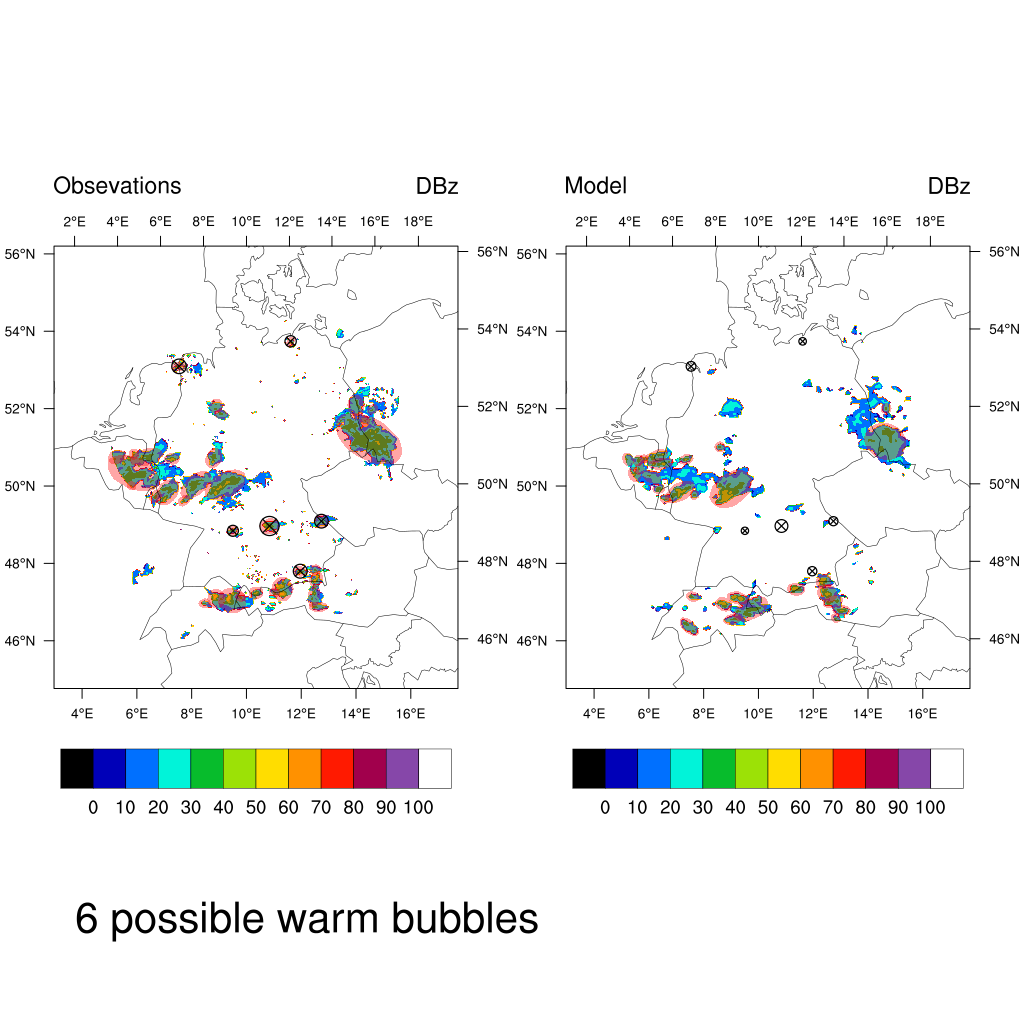
\includegraphics[width=\linewidth,trim=0 200 0 210,clip=]{bubble_plot.png}
  }
  \caption{\label{fig:bub6}Example for detected elliptical isolated precipitation objects (red semi-transparent ellipses) in observed (left) and simulated (right) composites of
  reflectivity (colors, dBZ). If observed objects are missing in the model and if these are not ``too big'' and not ``too small'' and are isolated
  from other observed objects (encircled black crosses), artificial ``warm bubbles'' are added to the model's temperature field in the PBL to trigger the missing convective cells.}
\end{figure}

\subsection{General description}

\labelsec{sec:warmbub:gen}

Simulations of case studies with convection-allowing grid spacings (~2\,km) are able to produce realistic convective
dynamics when the atmospheric profiles of humidity, temperature and wind match the observed conditions.
However, these simulations are often not able to capture the process that triggers the convective dynamics,
because relevant processes might be active below the model resolution.
Convection in idealized or ``forced'' real case studies is typically initiated by localized perturbations in the temperature and humidity profiles,
so-called ``warm bubbles'', which are artificially introduced at the beginning of the simulations (\citeNPK{weisman1982}) or any other appropriate time.
 
Similarly as with such case studies we observe that convection-allowing NWP produces realistic convective dynamics,
but may miss the convective trigger in many occasions. Missing the trigger deteriorates not only the prediction but also the assimilation.
For example, if the trigger is missed in all ensemble members, the LETKF (and many other ensemble assimilation techniques)
cannot recover the convective dynamics in the analysis. This limitation of ensemble methods is caused by the strong non-linearity of convection,
so that a convective cell cannot be reconstructed from non-convective members. As a result, NWP might miss large and long-lived convective cells,
even when we are certain of their existence from the radar signal.

We propose to use ``automatic'' warm bubbles to initiate convective cells that are missed in model runs 
but their existence is certain from radar observations. For data assimilation these are the cycled ``first guess'' forecasts.
While in case studies the researchers manually decide where to introduce warm bubbles,
this strategy is not feasible for an operational NWP with, e.g., a 40-member ensemble.
We have designed instead an automatic detection/triggering algorithm that decides where to initiate warm bubbles in the model.
The detection/triggering algorithm is based on the comparison of radar observation composites with their  simulated model counterparts.

The detection/triggering algorithm runs in each ensemble model run, independently of other members.
Warm bubbles are triggered in all ensemble members because we expect that bubbles produce realistic
convection only in members with the right pre-convective environment.
Those more realistic members are closer to the radar observations after the introduction of the bubbles and therefore
carry more weight in the subsequent assimilation analysis.
The introduction of warm bubbles has thus the potential not only to recover missed convective cells,
but also to improve the atmospheric state in the assimilation cycle.
The warm bubble analysis is performed in regular time intervals, typically every 10 to 15 minutes. This time span allows for the full early development of convective cells,
so that warm bubbles may not be triggered twice if the first was successful.

While similar in the general concept to the traditional Latent Heat Nudging (LHN) method, there are some significant differences:
\begin{itemize}
\item LHN adjusts precipitation, not radar reflectivity.
\item LHN does this continuously in every model timestep and in the whole domain, but applies rather small temperature and moisture increments continuously.
\item LHN is thermodynamically symmetric, because it can also suppress excess precipitation by negative increments.
\item The bubble generator can only create missing convective cells in simulation, it cannot destroy wrong cells.
\item The bubble generator applies large increments in a short time and waits for the model to react until the next analysis 10 to 15 minutes later.
\item In LHN, the increments are directly proportional to the precipitation rate difference (obs-model), whereas
  the properties of new bubbles (amplitude, size) are pre-selected by the user and do not depend on any reflectivity differences.
\item While LHN may be applied to all precipitation events in general, the bubble generator is especially tailored to
  intense, longlived, isolated and relatively small convective cells, such as rotating supercells. Such events are known
  to be problematic in LHN.
\end{itemize}
Conceptually, the bubble generator and LHN may be used together, but this requires further testing and tuning.


\subsection{Detecting missing cells in EMVORADO}

\labelsec{sec:warmbub:impl}

The bubble generator is active if \srcform{ldo_bubbles=.TRUE.} and \srcform{lreadmeta_from_netcdf=.TRUE.} in \srcform{/RADARSIM_PARAMS/}.
The latter namelist also defines the governing parameters for the cell object detection algorithm, which is described below,
as well as the properties of the ``warm bubbles'', see Table~\ref{tab:radarsimparams}.
The bubble parameters have similar meaning as corresponding parameters
in the COSMO idealized framework (\citeNPK{blahak2015b}).
Table~\ref{tab:bubtypical} shows a typical configuration for a 2-km-scale model.
These parameters are equal for all automatic bubbles and are automatically transferred to the hosting model along
with position- and time information.
See Sections~\ref{sec:warmbub:implcosmo} and~\ref{sec:warmbub:implicon} for further processing in COSMO and ICON.

The current detection algorithm typically works on the 2D composite reflectivity from radar scans with 0.5\grad elevation angle
(\srcform{eleind_for_composite_bub_glob=1} or \srcform{rs_meta($i$)\%eleind_for_composite_bub=1}),
interpolated to the COSMO-model grid. The compositing method has been described in Section~\ref{sec:intro:compo}.
For the German radar network, this composite covers all Germany and part of the neighboring countries as
shown in Fig.~\ref{fig:bub6}. The cell-detection algorithm searches for continuous regions above the
threshold $Th_1$, checking for East-West/North-South- and diagonal connected pixels.
We impose two conditions for a continuous region to be defined as a convective feature:
it encompasses at least the area $A_1$, and at least the area $A_2$ is above a higher threshold $Th_2$ (cell cores).
Once a convective feature is detected we use principal component analysis to find the best
ellipse that matches the region. The ellipses are then enlarged by multiplying the axis length by a factor $m_{en}$,
and/or by adding some distance $m_{add}$ to the axis. This option has been introduced to avoid bubbles being
triggered too close to existing developing convection. A typical set of parameters is summarized in Table~\ref{tab:bubtypical}
and connected to their respective namelist parameters in \srcform{/RADARSIM_PARAMS/}.
In this example, the parameters for model and observations are set equal and chosen in a way to detect intense
small-scale convective cells. We have also considered the possibility that observation parameters
are more restrictive than those for the model, so that we can broadly speak of convective cells in
observations and convective features in the model. This depends on the model's ability to simulate
very high reflectivities and will differ from model to model.

The triggering algorithm aims to initiate convection in regions where convective cells are observed but
there are no convective features in the model. With this idea, the algorithm searches for ellipses
identified by the detection algorithm in the observations that do not overlap with ellipses in the model.
We also impose that the observation ellipses are small (large axis smaller than some length, e.g. $75\,$km)
The last two conditions were introduced for the few occasions in which the model misses large
convective systems, because we think that the assimilation algorithm (LETKF) is more appropriate
to deal with them than the warm bubbles.

Warm bubbles are introduced at the location of observed convective cells with no model counterpart,
as proposed by the triggering algorithm. The bubbles of type \srcform{'cos-instant'} instantaneously increases
the temperature, while the bubbles of type \srcform{'cos-hrd'} apply a certain heating
rate $\dot{T}$ over a certain time interval $\Delta t_{heat}$. Optionally, the relative humidity is increased to keep it constant during heating.
This is done in a region centered on the ellipse center
in the horizontal and at a low height, e.g., $H_{bub}=2\,$km above ground level.
The heated region has a fixed ellipsoid shape with certain radii $r_{x,y}$ (e.g., 10\,km) for both horizontal main axes,
and a radius $r_Z$ (e.g., 2\,km) for the vertical axis.  The maximum temperature disturbance $\Delta T$ (e.g., 3.0\,K)
is at the center and it decreases towards the ellipsoids borders following a cosine function (\citeNPK{weisman1982}).
We have observed that these perturbations are effective in triggering convection while larger
perturbations are equally effective but generate too many pressure waves above the tropopause.

The above configuration of parameters for the warm bubble algorithm is rather intrusive,
as it produces around five warm bubbles in convective situations every time that the algorithm is called. 
This aggressive combination is thus appropriate to use warm bubbles as small-scale inflation method.
Other tests with more conservative approaches (~1 bubbles per call using a less restrictive criteria
for convective features in the model) showed that even when warms bubbles were able to recover some
convective cells that were missed in the reference runs, the resulting changes in FSS scores were small.
We believe that the small changes in FSS may be explained by the fact that this verification metric is
mostly determined by large structures that are mostly unaffected by the warm bubbles. 

Automatic bubbles might be optionally advected downstream for a distance that corresponds to a certain amount of time $\Delta t_{advect}$, to compensate
for the effect that it takes time for the bubble to rise above the boundary layer into
the tropospheric free flow. The advection velocity is computed as the local average windspeed
between two heights $H_{lower}$ and $H_{upper}$. The bubble triggering time itself is not delayed.

Optionally, white noise of a relative level $\alpha_{noise}$ (between 0 and 1) might be superimposed
on the bubbles to break their rotational symmetry a bit.

In case of asynchonous radar IO, there is a possibility to delay the transfer of the information about detected
missing cells from the output PEs to the compute PEs by a certain amount of time (\paramform{t_offset_bubble_trigger_async}). This allows the compute PEs to
continue model integration while missing cells are detected. Otherwise, compute PEs would have to wait until completion of
the bubble search on the IO PEs, which would destroy the runtime advantage of asynchronous IO. However, this comes at the expense of
a delayed bubble triggering. The bubble position will be advected downstream similar as and on top of $\Delta t_{advect}$.

\setlength{\lenspeins}{\linewidth*\real{0.22}}
\setlength{\lenspzwei}{\linewidth*\real{0.07}}
\setlength{\lenspdrei}{\linewidth*\real{0.11}}
\setlength{\lenspvier}{\linewidth*\real{0.42}}
\setlength{\extrarowheight}{0.25\baselineskip}

\begin{table}[h]
\caption{\label{tab:bubtypical}Typical parameters to configure the warm bubble generator in a 2-km-scale model. Cf. Table~\ref{tab:radarsimparams}.}
\begin{tabular}{|p{\lenspeins}|>{\centering}p{\lenspzwei}|>{\centering}p{\lenspdrei}|>{\centering}p{\lenspdrei}|p{\lenspvier}<{\vspace*{\extrarowheight}}|}
\hline
     & \textbf{Unit} & \textbf{Model} & \textbf{Observ.} &  \textbf{Param. in \srcform{/RADARSIM_PARAMS/}}\\
\hline
\hline
\multicolumn{2}{|l|}{\textbf{Detection parameter}} & \multicolumn{3}{l|}{}          \\\hline
$Th_1$     & dBZ     &     25       &     25   & threshold_mod(1), threshold_obs(1) \\\hline
$Th_2$     & dBZ     &     30       &     30   & threshold_mod(2), threshold_obs(2) \\\hline
$A_1$      & m$^2$   &     135E6    &   135E6  & areamin_mod(1), areamin_obs(1)     \\\hline
$A_2$      & m$^2$   &     35E6     &   35E6   & areamin_mod(2), areamin_obs(2)     \\\hline
$m_{en}$   &   -     &     1.0      &    1.0   & mult_dist_mod, mult_dist_obs       \\\hline
$m_{add}$  &   m     &     10000    &   10000  & add_dist_mod, add_dist_obs         \\\hline
\hline
\multicolumn{2}{|l|}{\textbf{Bubble parameter}}  &   \multicolumn{3}{l|}{}                  \\\hline
Type    &  ''    &    'cos-hrd' &     -    &  bubble_type ('cos-instant' or 'cos-hrd')  \\\hline
$r_{X,Y}$    &  m    &     10000    &     -    &   bubble_radx, bubble_rady   \\\hline
$r_{Z}$      &  m    &     2000     &     -    &  bubble_radz   \\\hline
$H_{bub}$        &  m    &     2000     &     -    &  bubble_centz   \\\hline
$\delta T$   &  K    &     3.0      &     -    &  bubble_dT ('cos-instant')  \\\hline
$\dot{T}$   &  K/s    &     0.04      &     -    &  bubble_heatingrate ('cos-hrd')  \\\hline
$\Delta t_{heat}$  &  s    &     200.0     &     -    &  bubble_timespan   \\\hline
If to hold RH constant   &  -    &     .TRUE.      &     -    &   bubble_holdrhconst  \\\hline
Main axis rotation   &  \grad    &     0.0      &     -    &   bubble_rotangle  \\\hline
If to add noise   &  -    &     .FALSE.      &     -    &   bubble_addnoise  \\\hline
$\alpha_{noise}$   &  -    &     0.1      &     -    &   bubble_dT_noise  \\\hline
$\Delta t_{advect}$   &  s    &     300.0    &     -    &   dt_bubble_advect  \\\hline
$H_{lower}$   &  m    &     3000.0      &     -    &   zlow_meanwind_bubble_advect  \\\hline
$H_{upper}$   &  m    &     6000.0      &     -    &   zup_meanwind_bubble_advect  \\\hline
\end{tabular}
\end{table}


\subsection{Implementation in COSMO}
\labelsec{sec:warmbub:implcosmo}

Generally, the properties of artificial convection triggers can be defined in two ways in COSMO: automatically via EMVORADO bubble generator or
manually via namelist parameters defined in the \srcform{/ARTIFCTL/} namelist. Details are
described in the COSMO documentation for idealized simulations \citeP{blahak2015b}, although
the part for the artificial convection triggers might also be applied in real-case simulations.
Convection triggers might be local disturbances of the atmospheric and/or soil initial state ($T$, moisture), or
local (in space and time) heating/moistening rate disturbances in atmosphere and/or soil.

In general, the parameters for the convection triggers in \srcform{/ARTIFCTL/} are
lists for up to \srcform{ntempdist_max} disturbances, the first element defines the first bubble, the
second element the second and so on, and there is a master switch list \srcform{ltempdist} for each disturbance.
For example, if \srcform{ltempdist}=.TRUE., FALSE., \dots), only the first bubble in all the parameter lists
will be activated. The type for each disturbance is defined using a certain name, e.g., \srcform{'cos'} ($\cos^2$ instantaneous bubble), \srcform{'cos-hrd'} ($\cos^2$ heating rate) or
\srcform{'cos-soil'} ($\cos^2$ disturbance in the soil), \srcform{'hotspot-soil'}.  \srcform{'cos-instant'} equals \srcform{'cos'}, but is
coded internally as a 1-timestep heatingrate for technical reasons.
If the COSMO binary is compiled with EMVORADO,
these disturbances can be also used in real cases by setting \srcform{ldo_bubbles_manual=.TRUE.} in \srcform{/RADARSIM_PARAMS/}.

The bubble informations from the automatic bubble generator are inserted into the
above \srcform{/ARTIFCTL/} disturbance lists starting
at the position $i$ of the first \srcform{ltempdist$(i)$}=.FALSE. element, i.e., after any ``manual'' bubbles. Thus,
manual and automatic bubbles may be combined.

For automatic bubbles, only the types \srcform{'cos-instant'} or \srcform{'cos-hrd'} can be chosen in the EMVORADO namelist. Other disturbance
types available in \srcform{/ARTIFCTL/} would not make sense in this
context. The bubble properties coming from EMVORADO are equal for all automatic bubbles
and are automatically filled into the above \srcform{/ARTIFCTL/} lists at the appropriate model time(s).
This information is evaluated in each model time step by the COSMO procedure \srcform{set_artif_heatrate_dist()} to superimpose disturbances
at the desired locations and times.


\subsection{Implementation in ICON}
\labelsec{sec:warmbub:implicon}

While COSMO's flexible framework for idealized test cases allowed to use it's part for idealized
convection triggers also in real-case simulations, this is currently not possible in ICON.
Here, an own trigger procedure \srcform{set_artif_heatrate_dist()} from module \srcform{mo_emvorado_warmbubbles.f90} is evaluated immediately after the microphysics part of
the time stepping, alongside the Latent Heat Nudging with it's $T$ and $RH$ increments.

Only bubbles of types \srcform{'cos-instant'} or \srcform{'cos-hrd'} are implemented (namelist parameter \paramform{bubble_type}).

Random noise on the bubbles is not yet implemented in ICON, so that the EMVORADO parameters
\srcform{bubble_addnoise} and \srcform{bubble_dT_noise} have no effect.

\clearpage

\section{For developers}

\labelsec{sec:devel}


\subsection{Implementing EMVORADO into hosting NWP models}

\labelsec{sec:impl}

EMVORADO itself is a collection of Fortran2003 modules, and each module name starts with the keyword \srcform{radar_}.
There is also a Fortran90  \srcform{inlcude}-file named \srcform{radar_elevations_precipscan.incf} which contains
the nominal elevation values as function of azimuth index for the horizon-following ``precipitation scans'' of DWD for
each of the German radar stations (station ID's).
The code in this file is the core of a \mbox{\srcform{SELECT CASE (rs_meta($I$)\%station_id)}} statement and
is \srcform{\#include}'d into subroutine \srcform{get_elarr_precipscan()} of \srcform{radar_obs_meta_list.f90}.
The code for this file has been created using the script \srcform{format_precipscan_f90} of U.~Blahak and
is based on the INPUT text file \srcform{elevations_precipscan.txt}, which has been provided by DWD's radar applications unit.

Important for the implementation/coupling of EMVORADO in a numerical NWP model are
\begin{itemize}
\item several initialization routines from \srcform{radar_interface.f90} which are called once during model initialization from
  the numerical model.
\item the generic organizational subroutine \srcform{organize_radar()} in module \srcform{radar_src.f90}. This is the
  top-layer interface for the radar simulation in each model timestep and is directly called once for further initializations ('init' stage) and in the model timeloop ('compute' stage).
\item \srcform{radar_mie_iface_cosmo.f90} and \srcform{radar_mie_meltdegree.f90}: interface procedures
  to compute grid point values (reflectivity, hydrometeor fall speed), at the moment only for
  the COSMO- and ICON cloud microphysics schemes, taking into account melting hydrometeors.
  These interface procedures are associated with step~1 of EMVORADO.
\item \srcform{radar_namelist_read.f90} contains the subroutine \srcform{input_radarnamelist()} to
  read the \srcform{/RADARSIM_PARAMS/} namelist(s).
\item \srcform{radar_src.f90} also contains the generic interface routines for step~2 of the operator, which
  are directly called from \srcform{organize_radar()}.\\
  Further, this module includes the code for computing \srcform{superobservations}
  and for output of \srcform{volume data}, \srcform{feedback files} and \srcform{composites} (grib2).
\item \srcform{radar_obs_meta_read.f90} contains the code for reading the radar station metadata from observation files, if any are used.
\item \srcform{radar_obs_meta_list.f90} contains the background metadata lists for each known
  ``country'' (\srcform{icountry}) and radar station.
\item \srcform{radar_obs_data_read.f90} contains the code for \srcform{reading observational data}.
\item There are model-specific procedures (interpolation to/from model grid, time housekeeping, parallelization, etc.)
  in the module \srcform{radar_interface.f90}.
  This module is a two-way connection and generally differs from model to model:
  On the one hand, it provides the specific code for some generic
  model-related procedures used in \srcform{radar_src.f90} associated with the model grid (interpolation),
  the time-housekeeping, the profiling (``timing'') and the MPI-parallelization.
  It may use specific routines from the model itself and connects EMVORADO with the model fields and some global model parameters.
  On the other hand, it provides an operator-specific initialization routine and some parameters to be called/used
  in the hosting model.
\item For ICON, the \srcform{radar_interface.f90} module has been split in two modules, named \srcform{radar_interface.f90} and \srcform{radar_mpi_init_icon.f90}.
\item In \srcform{radar_data_namelist.f90}, the name and path for the EMVORADO namelist file can be adapted from \srcform{INPUT_RADARSIM} / \srcform{NAMELIST_EMVORADO} to
  differing naming conventions in other models. Similarly, the name and path to the namelist control output (\srcform{YUSPECIF_RADAR} / \srcform{nml.emvorado.log}) can be adapted.
\end{itemize}
The actual implementation of the calls to the top-level procedures of these modules depends on the hosting numerical model.


\newpage

\subsection{Implementation documentation for COSMO}

\labelsec{sec:implcosmo}

This section describes how the general implementation aspects described in the last section~\ref{sec:impl}
are actually implemented in the COSMO-model. Here:
\begin{itemize}
\item Calls to several initialization routines from \srcform{radar_interface.f90} from
  the main program \srcform{lmorg}. These are described below in Section~\ref{sec:impltop}.
\item Calls of the generic organizational subroutine \srcform{organize_radar()} from module \srcform{radar_src.f90}
  from \srcform{lmorg} for the 'init' and 'compute' stages, also described below in Section~\ref{sec:impltop}.
\item Specific calls to interface routines from \srcform{radar_mie_iface_cosmo.f90} and \srcform{radar_mie_meltdegree.f90} or step~1 of the operator described below in Section~\ref{sec:impl1}.
\item Traditional gridpoint output using the same interface routines to reflectivity and hydrometeor
  fallspeed than for step~1 of the operator (Section~\ref{sec:impltradi}).
\end{itemize}
Along with the calling sequences, a rough description of the specific tasks of
the interface routines is also given in the next sections.


\subsubsection{The top-level interface to COSMO}

\labelsec{sec:impltop}

At model initialization stage, two EMVORADO-specific sections are added for initializing
its MPI-parallelization, the optional asynchroneous radar-IO, reading the \srcform{/RADARSIM_PARAMS/} namelist,
and connecting the prognostic model fields with correscponding pointers inside EMVORADO.

The computing- and output-stages (steps~1 and~2) are performed in every timestep by a call to \srcform{organize_radar('compute')}
after the update of the model variables by physics and dynamics. EMVORADO uses timestep ``nnow'' of the model fields, consistent with the ``normal'' grib output.

In the following, we give a schematic of the calling sequence of the top-layer interface to EMVORADO in the main program \srcform{lmorg}
for the initialization stage and the time-loop, taking into account the optional asynchroneous radar-IO if
\srcform{nprocio_radar~$>$ 0} is chosen in namelist \srcform{/RUNCTL/}. The blue color highlights the
additional EMVORADO-related code blocks, which are enclosed by \srcform{\#ifdef RADARFWO} in the COSMO source code. Black indicates ``normal'' COSMO code for better orientation:

\begin{algorithm}[H]
\DontPrintSemicolon
\SetKwIF{If}{ElseIf}{Else}{IF}{THEN}{ELSE IF}{ELSE}{END IF}

\KwSty{CALL organize_setup}
\vspace*{-0.5em}
\DataSty{
  \parbox[t]{\linewidth}{
    \begin{itemize}[topsep=0pt,itemsep=0pt,partopsep=0pt,parsep=0pt]
    \item split \KwSty{icomm_compute} from \KwSty{icomm_world} and define \KwSty{lcompute_pe}, \KwSty{icomm_cart} (\KwSty{CALL init_procgrid} from environment.f90)
    \item \textcolor{blau}{split \KwSty{icomm_computeio} from \KwSty{icomm_world}, so that \KwSty{icomm_computeio = icomm_compute + icomm_asynio}}
    \item \textcolor{blau}{if \KwSty{nprocio_radar $>$ 0}, additional PEs for asynchroneous radar-IO are allocated at the end of \KwSty{icomm_world}.
      These are not part of \KwSty{icomm_computeio}.}
    \end{itemize}
}} \;
\dots \;
\BlankLine
\BlankLine
\KwSty{CALL organize_dynamics('input')} \;
\BlankLine
\dots \;
\BlankLine
\BlankLine
\KwSty{CALL organize_physics('input')} \;
\BlankLine
\dots \;
\BlankLine
\BlankLine
\textcolor{blau}{
\KwSty{CALL get_model_config_for_radar}
\vspace*{-0.5em}
\DataSty{
  \parbox[t]{\linewidth}{
    \begin{itemize}[topsep=0pt,itemsep=0pt,partopsep=0pt,parsep=0pt]
    \item because of grid point reflectivity output
    \end{itemize}
}} \;
%%%
\uIf{luse_radarfwo}{
\KwSty{CALL prep_domains_radar} \;
\KwSty{CALL prep_domains_radar_nml} \;
\KwSty{CALL init_radar_mpi}
\vspace*{-0.5em}
\DataSty{
  \parbox[t]{\linewidth}{
    \begin{itemize}[topsep=0pt,itemsep=0pt,partopsep=0pt,parsep=0pt]
    \item First initialization step of EMVORADO: internal MPI
    \item If asynchroneous radar-IO (\KwSty{nprocio_radar $>$ 0}):
      \begin{itemize}[topsep=0pt,itemsep=0pt,partopsep=0pt,parsep=0pt]
      \item split \KwSty{icomm_radario} from \KwSty{icomm_world}, so that \KwSty{icomm_radario = icomm_world - icomm_compute - icomm_asynio}. This is the communicator for the extra radar-IO-PEs. Sets \KwSty{lradario_pe = .TRUE.} on \KwSty{icomm_radario}.
      \item split \KwSty{icomm_radar} from \KwSty{icomm_world}, so that \KwSty{icomm_radar = icomm_world - icomm_asynio}. This is the common communicator of the compute-PEs and the radar-IO-Pes and is used for data exchange between the two. Also, sets \KwSty{lradar_pe = .TRUE.} on \KwSty{icomm_radar}.
      \item as a result, \KwSty{icomm_radar = icomm_compute + icomm_radario} and \KwSty{lradar_pe = lcompute_pe or lradario_pe}.
      \end{itemize}
    \item If synchroneous radar-IO (\KwSty{nprocio_radar $=$ 0}):
      \begin{itemize}[topsep=0pt,itemsep=0pt,partopsep=0pt,parsep=0pt]
      \item set \KwSty{icomm_radar = icomm_compute} and \KwSty{icomm_radario = icomm_compute}, sets \KwSty{lradar_pe = .TRUE.} and \KwSty{lradario_pe = .TRUE.} on \KwSty{icomm_compute}
      \end{itemize}
    \end{itemize}
}} \;
}
\Else{
\KwSty{CALL init_radar_mpi_light} \;
\KwSty{lradar_pe = .FALSE.} \;
\KwSty{lradario_pe = .FALSE.}
\vspace*{-0.5em}
\DataSty{
  \parbox[t]{\linewidth}{
    \begin{itemize}[topsep=0pt,itemsep=0pt,partopsep=0pt,parsep=0pt]
    \item Necessary because of possible grid-point reflectivity output
    \end{itemize}
}} \;
}
}
\BlankLine
\BlankLine
\BlankLine
\KwSty{CALL organize_data('input')}
\vspace*{-0.5em}
\DataSty{
  \parbox[t]{\linewidth}{
    \begin{itemize}[topsep=0pt,itemsep=0pt,partopsep=0pt,parsep=0pt]
    \item read namelists for IO, also for lartif_data
    \end{itemize}
}} \;
\BlankLine
\dots \;

\end{algorithm}


\begin{algorithm}[t]
\DontPrintSemicolon
\SetKwIF{If}{ElseIf}{Else}{IF}{THEN}{ELSE IF}{ELSE}{END IF}

\KwSty{CALL organize_data('init')}
\vspace*{-0.5em}
\DataSty{
  \parbox[t]{\linewidth}{
    \begin{itemize}[topsep=0pt,itemsep=0pt,partopsep=0pt,parsep=0pt]
    \item \textcolor{blau}{setup dbz_meta-structure for grid point dBZ-output},
    \item \textcolor{blau}{pre-compute needed MIE-lookup tables by \KwSty{CALL init_lookup_mie}},
    \item \KwSty{CALL mpe_io_init}: \textcolor{blau}{split \KwSty{icomm_compute} from \KwSty{icomm_computeio} instead of \KwSty{icomm_world}}
    \end{itemize}
}} \;

\dots \;
\BlankLine
\BlankLine
\If{lcompute_pe}{
\vspace*{-0.5em}
\DataSty{
  \parbox[t]{\linewidth}{
    \begin{itemize}[topsep=0pt,itemsep=0pt,partopsep=0pt,parsep=0pt]
    \item allocate model fields
    \item compute constant fields (metrical \srcform{terms}, srcform{rlat}, srcform{rlon})
    \item read initial data
    \end{itemize}
}} \;
}

\BlankLine
\dots \;
\BlankLine
\BlankLine

\textcolor{blau}{
\If{lradar_pe}{
  \uIf{luse_radarfwo}{
    \KwSty{CALL organize_radar('init')}
    \vspace*{-0.5em}
    \DataSty{
      \parbox[t]{\linewidth}{
        \begin{itemize}[topsep=0pt,itemsep=0pt,partopsep=0pt,parsep=0pt]
        \item Second initialization step of EMVORADO: namelist and pointers to the COSMO model fields
          \begin{itemize}[topsep=0pt,itemsep=0pt,partopsep=0pt,parsep=0pt]
          \item read and distribute radar namelist \srcform{/RADARSIM_PARAMS/} to all PEs in \KwSty{icomm_radar},
          \item this requires reading of the header information from all radar observation input files if namelist parameter lread_meta_from_netcdf = .TRUE.,
          \item check radar namelist settings and compute additional parameters,
          \item control output of radar namelist to file \srcform{YUSPECIF_RADAR},
          \item \KwSty{CALL get_model_config_for_radar},
          \item setup radar-composite metadata,
          \item pre-compute needed MIE lookup tables in parallel over all PEs in icomm_radar,
          \item \KwSty{CALL get_model_hydrometeors},
          \item \KwSty{CALL get_model_variables},
          \item \KwSty{CALL alloc_aux_model_variables}.
          \end{itemize}
        \end{itemize}
    }} \;
    \KwSty{CALL crosscheck_domains_radar_nml} \;
  }
  \Else{
    \KwSty{CALL get_model_config_for_radar}
    \vspace*{-0.5em}
    \DataSty{
      \parbox[t]{\linewidth}{
        \begin{itemize}[topsep=0pt,itemsep=0pt,partopsep=0pt,parsep=0pt]
        \item This is necessary for the separate grid-point reflectivity output via \srcform{/GRIBOUT/} namelist(s) in case
          of \srcform{luse_radarfwo = .FALSE.}, i.e. if the full EMVORADO is not used.
        \end{itemize}
    }} \;
  }
}}
\BlankLine
\dots \;
\end{algorithm}

\begin{algorithm}[H]
\DontPrintSemicolon
\SetKwIF{If}{ElseIf}{Else}{IF}{THEN}{ELSE IF}{ELSE}{END IF}

\uIf{lcompute_pe}{
  \SetKwFor{For}{timeloop: DO}{}{END DO timeloop}
  \For{ntstep=1,nstop}{
    \vspace*{-0.5em}
    \DataSty{
      \parbox[t]{\linewidth}{
        \begin{itemize}[topsep=0pt,itemsep=0pt,partopsep=0pt,parsep=0pt]
        \item Integrate model for one timestep
        \end{itemize}
    }}
    \dots \;
    \BlankLine
    \textcolor{blau}{
      \KwSty{CALL organize_radar('compute')}
      \vspace*{-0.5em}
      \DataSty{
        \parbox[t]{\linewidth}{
          \begin{itemize}[topsep=0pt,itemsep=0pt,partopsep=0pt,parsep=0pt]
          \item Steps~1 and~2 of EMVORADO for each radar station at each individual output time.
          \item If \KwSty{nprocio_radar $>$ 0}:
            \begin{itemize}[topsep=0pt,itemsep=0pt,partopsep=0pt,parsep=0pt]
            \item sends the simulated radar data from the compute-PEs to the radar-IO-PEs via \KwSty{icomm_radar} and exits.
            \end{itemize}
          \item If \KwSty{nprocio_radar $=$ 0}:
            \begin{itemize}[topsep=0pt,itemsep=0pt,partopsep=0pt,parsep=0pt]
            \item collects (re-distributes) the simulated radar data on one compute-PE per station
            \item reads radar observations if needed
            \item computes radar composites if desired
            \item detects the locations for artificial warm bubbles if desired
            \item outputs radar volume data and/or feedback files for data assimilation
            \end{itemize}
          \end{itemize}
      }}
    }
    \dots \;
    \BlankLine
    \If{output-time}{
      \uIf{lasyn_io}{
        \vspace*{-0.5em}
        \DataSty{
          \parbox[t]{\linewidth}{
            \begin{itemize}[topsep=0pt,itemsep=0pt,partopsep=0pt,parsep=0pt]
            \item Send model field data to the asynchroneous model output PEs (non-blocking) and continue
          \end{itemize}
      }} \;
      }
      \Else{
        \vspace*{-0.5em}
        \DataSty{
          \parbox[t]{\linewidth}{
            \begin{itemize}[topsep=0pt,itemsep=0pt,partopsep=0pt,parsep=0pt]
            \item Do the output of model fields on PE 0
            \end{itemize}
        }} \;
      }
    }
  }
}

\BlankLine
\BlankLine
\textcolor{blau}{
  \uElseIf{lradario_pe \KwSty{and} nprocio_radar $>$ 0}{
    \SetKwFor{For}{timeloop_2: DO}{}{END DO timeloop_2}
    \For{ntstep=1,nstop}{
      \KwSty{CALL organize_radar('compute')}
      \vspace*{-0.5em}
      \DataSty{
        \parbox[t]{\linewidth}{
          \begin{itemize}[topsep=0pt,itemsep=0pt,partopsep=0pt,parsep=0pt]
          \item This is a call on pure radar output PEs, so \KwSty{CALL organize_radar} just waits to receive
            simulated radar data from the compute-PEs via \srcform{icomm_radar}, one output-PE per station.
          \item Receives from the corresponding \KwSty{CALL organize_radar} in the model timeloop above, therefore the exact same time stepping is needed.
          \item Does not use any model fields, just needs to know about the actual model time,
          \item reads radar observations if needed,
          \item computes radar composites if desired,
          \item detects the locations for artificial warm bubbles if desired,
          \item outputs radar volume data and/or feedback files for data assimilation to \srcform{ydirradarout}.
          \end{itemize}
      }} \;
    }
  }
}

\BlankLine
\BlankLine
\Else(These are the asynchroneous model output PEs){
  \vspace*{-0.5em}
  \DataSty{
    \parbox[t]{\linewidth}{
      \begin{itemize}[topsep=0pt,itemsep=0pt,partopsep=0pt,parsep=0pt]
      \item Listen to receive and output model data records from the compute-PEs and
        wait for the next output messages,
      \item if model time is finished, stop listening.
      \end{itemize}
  }} \;
}
\end{algorithm}



\subsubsection{Implementation of step~1: grid point values of $Z_h$, polarization parameters and hydrometeor terminal fallspeed}

\labelsec{sec:impl1}

The corresponding subroutines \srcform{calc_dbz_vec_modelgrid()} ($Z_h$, polarization parameters), \srcform{calc_fallspeed_vec_modelgrid()} (terminal fallspeed) and \srcform{init_lookup_mie()} (initialization of lookup tables)
from \srcform{radar_mie_iface_cosmo.f90}
are called from step~2-routines from within EMVORADO, when $Z_h$, polarization parameters and/or hydrometeor fallspeed on the model grid is needed to be
interpolated to the radar bins.


\subsubsection{Implementation of step~2: volume scans of $Z_h$, polarization parameters and $v_r$}

\labelsec{sec:impl2}

All corresponding subroutines regarding interpolation from model grid to radar bins
are contained in \srcform{radar_src.f90} and are called from the top-level
EMVORADO routine \srcform{organize_radar()} during the \srcform{'compute'} stage, depending on the general
setup of EMVORADO. \srcform{organize_radar()} is called from the main program as described in Section~\ref{sec:impltop}.
\srcform{radar_src.f90} also contains the procedures for the different kinds of radar data output,

If observation files are used, the code for reading the station metadata and the actual radar observables
from the files is in \srcform{radar_obs_meta_read.f90} and \srcform{radar_obs_data_read.f90}.
\srcform{radar_obs_meta_list.f90} holds procedures for initial initialization of
the metadata type \srcform{rs_meta($i$)} depending on \srcform{icountry}, as well
as background metadata lists for each known radar station for cross-checking.

\subsubsection{Implementation of ``traditional'' grid point reflectivity ($Z_h$) output}

\labelsec{sec:impltradi}

The subroutines \srcform{calc_dbz_vec()}, \srcform{calc_fallspeed_vec_modelgrid()} and \srcform{init_lookup_mie()}
are also called at other places in COSMO in case of ``traditional'' grid point reflectivity and fallspeed output via \srcform{/GRIBOUT/} namelist.
This is needed if at least one of the shortnames \srcform{DBZ} (\srcform{yvarml}, \srcform{yvarpl}, or \srcform{yvarzl}), \srcform{DBZ_850} (\srcform{yvarml}), \srcform{DBZ_CMAX} (\srcform{yvarml}) and \srcform{DBZ_CTMAX} (\srcform{yvarml}) has been specified in the \srcform{/GRIBOUT/} namelists.
\begin{itemize}
\item \srcform{init_lookup_mie()} in \srcform{organize_data.f90}, section \srcform{'start'}, to prepare Mie- or T-matrix lookup tables if required by
  the choice \srcform{dbz\%itype_refl=1,5,6} in namelist \srcform{/GRIBOUT/}
\item \srcform{calc_dbz_vec_modelgrid()} in \srcform{calc_tracks.f90}
\item \srcform{calc_dbz_vec_modelgrid()} and \srcform{calc_fallspeed_vec_modelgrid()} in \srcform{src_output.f90}
\end{itemize}
By using these subroutines at these points, the grid point reflectivity output
has been extended by options for the Mie-, T-matrix and Rayleight-Oguchi-methods \srcform{dbz\%itype_refl=1,3,5,6} from EMVORADO, as already
mentioned in Section~\ref{sec:intro}.
For backwards compatibility, the previous method from \srcform{pp_utilities.f90}
is available as option \srcform{dbz\%itype_refl=4}.

For developers, hydrometeor fallspeed is available via the shortname \srcform{DUMMY_1} and the Mie two-way attenuation coefficient (\srcform{dbz\%itype_refl=1,5,6})
via the shortname \srcform{DUMMY_2}.


\subsection{Implementation documentation for ICON}

\labelsec{sec:implicon}

TODO

\subsection{Recipe to implement new namelist parameters into \srcform{/RADARSIM_PARAMS/}}

\labelsec{sec:devel:newnml}

\begin{aufzaehlung}
\item Add declaration statement to module \srcform{radar_data_namelist.f90}.
\item Add corresponding component to declaration of derived type \srcform{glob_nml_type} in \srcform{radar_data_namelist.f90}.
\item Add corresponding code line to subroutines \srcform{store_domain_radar_nml} and \srcform{switch_to_domain_radar_nml} in \srcform{radar_data_namelist.f90}. Existing lines for other namelist parameters may serve as an orientation.
\item Does your parameter have to be different for different model domains? If yes, add a corresponding
check to subroutine \srcform{crosscheck_domains_radar_nml} in \srcform{radar_data_namelist.f90}.
\item Add default value, some cross-checks (if needed) and global MPI-distribution to subroutine \srcform{input_radarnamelist()} in module \srcform{radar_namelist_read.f90}. Note that the namelist is read from file several times
during the process, because the default of some parameters depends on the actual setting of other parameters. But if this
is not the case for your new parameter, simply add it to the first namelist reading pass.
\item Add control output for file \srcform{YUSPECIF_RADAR} / \srcform{nml.emvorado.log} near the end of subroutine \srcform{input_radarsim.f90}.
\end{aufzaehlung}

\subsection{Recipe to implement new type components into \srcform{rs_meta} }

\labelsec{sec:devel:newtypers}

The namelist parameter type instance \srcform{rs_meta} is of derived type \srcform{radar_meta_type}, which
is declared in module \srcform{radar_data.f90}.
\begin{aufzaehlung}
\item Add new component to declaration of derived type \srcform{radar_meta_type} in \srcform{radar_data.f90}.
\item Add corresponding copy line to subroutines \srcform{rsm_multitime2onetime} and \srcform{rsm_onetime2multitime} from \srcform{radar_data.f90}.
If your new component is an array where any of the dimensions is \srcform{nobstimes_max}, only the first element 
along this dimension is retained.
\item In module \srcform{radar_parallel_utilities.f90}, extent the derived MPI-type \srcform{mpi_radar_meta_typ}
in subroutine \srcform{def_mpi_radar_meta_type} by the size of your new component.
The existing code shows you how to do this: There are different blocks for the different
basic Fortran90 types, and you have to add the size (number of elements, not number of bytes!) of
your new component (might be a scalar with size 1 or an array) to the
\srcform{``blocklengths''} - counter before the corresponding \srcform{CALL MPI_TYPE_EXTENT()} statement.
\item If your new component is an array with \srcform{nobstimes_max} as any of the dimensions, use the local INPUT variable
\srcform{nobstimes_max_loc} in the \srcform{``blocklengths''} - statement instead.
\item In module \srcform{radar_namelist_read.f90}, add a control output line for file \srcform{YUSPECIF_RADAR} / \srcform{nml.emvorado.log} in the
subroutine \srcform{ctrl_output_rsmeta_nuspec_fwo()}.
\end{aufzaehlung}

\subsection{Recipe to implement new type components into \srcform{dbz_meta}}

\labelsec{sec:devel:newtypedbz}

The namelist parameter type instance \srcform{dbz_meta} is of derived type \srcform{t_dbzcalc_params}, which
is declared in module \srcform{radar_data.f90}.
\begin{aufzaehlung}
\item Add new component to declaration of derived type \srcform{t_dbzcalc_params} in \srcform{radar_data.f90}.
\item Add corresponding background default value to the declaration block of\\
  \srcform{ TYPE(t_dbzcalc_params), PARAMETER  :: dbz_namlst_d}\\
  in module \srcform{radar_data.f90}.
\item In module \srcform{radar_parallel_utilities.f90}, extent the derived MPI-type \srcform{mpi_dbzcalc_params_typ}
in subroutine \srcform{def_mpi_dbzcalc_params_type} by the size of your new component.
The existing code shows you how to do this: There are different blocks for the different
basic Fortran90 types, and you have to add the size (number of elements, not number of bytes!) of
your new component (might be a scalar with size 1 or an array) to the
\srcform{``blocklengths''} - counter before the corresponding \srcform{CALL MPI_TYPE_EXTENT()} statement.
\item In module \srcform{radar_namelist_read.f90}, add a control output line for file \srcform{YUSPECIF_RADAR} / \srcform{nml.emvorado.log} in the
subroutine \srcform{ctrl_output_dbzmeta_nuspec_fwo()}.
\end{aufzaehlung}

\subsection{Recipe to implement a new ``country''}

\labelsec{sec:devel:newcountry}

In the context of EMVORADO, a ``country'' denotes a set of metadata defaults for a group of similar radars.
This set serves as a background default for the station metadata \srcform{rs_meta} and, 
as mentioned earlier in Table~\ref{tab:radarsimparams}, may be chosen either globally by the parameter \srcform{icountry} or
individually for each station by \srcform{rs_meta(i)\%icountry}. The current choice of
countries is described in Table~\ref{tab:radarsimparams}.

In order to add a new option to \srcform{icountry}, the following steps are necessary:
\begin{itemize}
\item Add a background metadata list with allowed default scan strategies in \srcform{radar_obs_meta_list.f90}:
  \begin{itemize}
  \item \srcform{get_meta_proto_$<$newcountry$>$()}
  \item \srcform{get_meta_network_$<$newcountry$>$()}
  \item \srcform{get_meta_network_all()}
  \end{itemize}
\item Add a new metadata reader in the subroutine \srcform{read_meta_info_all()} in  \srcform{radar_obs_meta_read.f90}:
  \begin{itemize}
  \item \srcform{get_metadata_from_$<$newcountry$>$()}
  \end{itemize}
\item Add a new data reader in the subroutine \srcform{read_obs_rad()} in \srcform{radar_obs_data_read.f90}:
  \begin{itemize}
  \item \srcform{read_field_obs_$<$newcountry$>$()}
  \end{itemize}
\item Add new declarations in \srcform{radar_data_namelist.f90}:
  \begin{itemize}
  \item \srcform{nradsta_$<$newcountry$>$}
  \item \srcform{rs_meta_$<$newcountry$>$_proto}
  \item \srcform{rs_meta_$<$newcountry$>$(nradsta_$<$newcountry$>$)}
  \end{itemize}
\end{itemize}

\clearpage

\section{Acknowledgements}

It all started by two postdocs sitting in the same room at the Institute for Meteorology and Climate Research (IMK), Karlsruhe Institute of Technology (KIT).
Axel Seifert (IMK, nowadays DWD) worked on cloud microphysical parameterization schemes and needed a radar forward operator
to evaluate his developments by observations of a C-Band research radar. After his initial Mie-coding, Ulrich Blahak (IMK, nowadays DWD) took over and developed a code for grid point reflectivities.
The further development into the full EMVORADO with all its physical capabilities (and its tricks to be efficient at the same time) by Yuefei Zeng, Dorit Jerger and Ulrich Blahak at IMK
profited from a grant within the programme ``Extramural Research'' of the German Weather Service (DWD). During this whole time, we are indepted to Klaus D. Beheng (IMK) for his constant support, encouragement and many discussions
on cloud microphysics and radar meteorology.

During this process Ulrich Blahak moved from KIT to DWD, and EMVORADO profited from many valuable contributions and
discussions with numerous colleages from DWD (Christoph Schraff, Andreas Rhodin, Klaus Stephan, just to name a few). We thank also Daniel Leuenberger from MeteoSwiss for many very valuable discussions
and some initial code contributions to solve tricky MPI-problems. EMVORADO was brought into operational service at DWD for assimilation of $Z_h$ and $v_r$ in the regional NWP-models COSMO-D2 and ICON-D2 by contributions
of many DWD colleagues from project SINFONY and the data assimilation section. This profited also from research on radar data assimilation within the Hans-Ertel-Zentrum (HErZ) at the Meteorological Institute of Ludwig Maximilians University Munich (LMU).

Jeffrey Snyder and Jacob Carlin (NSSL, Oklahoma, USA) laid the foundations of the upgrade to dual polarimetric capabilities, which was taken over and continued by Jana Mendrok (DWD) with support from grant BL~945/2-1
by Deutsche Forschungsgemeinschaft (DFG) within the Priority Programme ``PROM''.

\newpage

\bibliographystyle{uliams_eng} 
\bibliography{emvoradoDocuBib}
\addcontentsline{toc}{section}{\bibname}


\end{document}



